\documentclass[a4paper, twoside, nobib]{tufte-book}


\hypersetup{colorlinks}% uncomment this line if you prefer colored hyperlinks (e.g., for onscreen viewing)

%%
% Book metadata
\title[A Physicist's Approach To Machine Learning -- Understanding The Basic Bricks]{A Physicist's \newline \noindent 
       Approach to \newline \noindent 
       Machine Learning \newline \noindent
       --  \newline \noindent
       Understanding  \newline \noindent
       The Basic Bricks}
\author[Christian Michelsen]{\newline \noindent 
        Christian Michelsen \newline \noindent 
        Niels Bohr Institute \newline \noindent 
        University of Copenhagen \newline }
\publisher[]{Supervisor: \newline \noindent 
           Troels Petersen \newline \noindent
           Niels Bohr Institute \newline \noindent
           University of Copenhagen}

%%
% If they're installed, use Bergamo and Chantilly from www.fontsite.com.
% They're clones of Bembo and Gill Sans, respectively.
%\IfFileExists{bergamo.sty}{\usepackage[osf]{bergamo}}{}% Bembo
%\IfFileExists{chantill.sty}{\usepackage{chantill}}{}% Gill Sans

%\usepackage{microtype}

% when using custom bibliography
\usepackage[square, numbers, nonamebreak]{natbib}
\bibliographystyle{abbrvnat}


%%
% Just some sample text
\usepackage{lipsum}

% package for quotes
\usepackage{epigraph}
\setlength\epigraphwidth{.8\textwidth}
% \setlength\epigraphrule{0pt}

%%
% For nicely typeset tabular material
\usepackage{booktabs}

% maths packages
\usepackage{amsthm,amssymb,amsmath}
\usepackage[mathscr]{eucal}

%%
% For graphics / images
\usepackage{graphicx}
\setkeys{Gin}{width=\linewidth,totalheight=\textheight,keepaspectratio}
\graphicspath{{graphics/}{{figures/}}}

% allow for dots in filename
\usepackage{grffile}


\usepackage{tikz}
\usepackage[subpreambles=true]{standalone}

% subcaption does not work with tufte
\usepackage[caption=false]{subfig}
% \usepackage[export]{adjustbox}


% The fancyvrb package lets us customize the formatting of verbatim
% environments.  We use a slightly smaller font.
\usepackage{fancyvrb}
\fvset{fontsize=\normalsize}

%%
% Prints argument within hanging parentheses (i.e., parentheses that take
% up no horizontal space).  Useful in tabular environments.
\newcommand{\hangp}[1]{\makebox[0pt][r]{(}#1\makebox[0pt][l]{)}}

%%
% Prints an asterisk that takes up no horizontal space.
% Useful in tabular environments.
\newcommand{\hangstar}{\makebox[0pt][l]{*}}

%%
% Prints a trailing space in a smart way.
\usepackage{xspace}

% add numbers to chapters, sections, subsections
\setcounter{secnumdepth}{2}
\setcounter{tocdepth}{2}

% Feyman diagrams
% \usepackage{tikz-feynman}
% \usepackage{feynman}

% lemmas and corrollaryies
% \newtheorem{theorem}{Theorem}[section]
% \newtheorem{corollary}{Corollary}[theorem]
% \newtheorem{lemma}[theorem]{Lemma}
\newtheorem{lemma}{Lemma}
\newtheorem{sublemma}{Lemma}[lemma]
\newtheorem{corollary}{Corollary}
\newtheorem{theorem}{Theorem}
\newtheorem{axiom}{Axiom}

% bold math
\usepackage{bm}

% for vector norms and abs
\newcommand{\abs}[1]{\lvert#1\rvert}
\newcommand{\norm}[1]{\lVert#1\rVert}

% allow first, second and third
\usepackage[super]{nth}

% % for using Inkscape plots
\usepackage{import}
\usepackage{xifthen}
\usepackage{pdfpages}
\usepackage{transparent}
\newcommand{\incfig}[1]{%
    \def\svgwidth{\columnwidth}
    \import{./figures/}{#1.pdf_tex}
}


%  units
\usepackage{siunitx}
\sisetup{seperr}
\DeclareSIUnit{\kroner}{kr.}
\DeclareSIUnit{\kr}{kr.}
\DeclareSIUnit{\Mkr}{M.kr.}


% custom subsubsection:

\titleclass{\subsubsection}{straight}
\titleformat{\subsubsection}%
  [hang]% shape
  {\normalfont\itshape}% format applied to label+text
  {\thesubsubsection}% label
  {1em}% horizontal separation between label and title body
  {}% before the title body
  []% after the title body



% \titleformat{\chapter}%
%   [display]% shape
%   {\relax\ifthenelse{\NOT\boolean{@tufte@symmetric}}{\begin{fullwidth}}{}}% format applied to label+text
%   {\itshape\huge\thechapter}% label
%   {0pt}% horizontal separation between label and title body
%   {\huge\rmfamily\itshape}% before the title body
%   [\ifthenelse{\NOT\boolean{@tufte@symmetric}}{\end{fullwidth}}{}]% after the title body

\usepackage[dvipsnames]{xcolor}
\definecolor{red} {RGB}{227, 26, 28}
\definecolor{blue}{RGB}{31, 120, 180}
\definecolor{green}{RGB}{51, 160, 44}
\definecolor{orange}{RGB}{255, 127, 0}
\definecolor{purple}{RGB}{106, 61, 154}

\definecolor{light-blue}{RGB}{166, 206, 227}
\definecolor{light-green}{RGB}{178, 223, 138}
\definecolor{light-purple}{RGB}{202, 178, 214}

\definecolor{viridis-light}{RGB}{252, 226, 63}
\definecolor{viridis-dark}{RGB}{59, 18, 72}





\definecolor{light-gray}{gray}{0.95}


% make a code environment
\newcommand{\code}[1]{\colorbox{light-gray}{\texttt{\detokenize{#1}}}}

% make quote signs
\newcommand{\q}[1]{``#1''}

% make Figure quote
\newcommand{\figref}[1]{Figure ~\ref{#1}}

% avoid problems with autocite not properly defined
\newcommand{\autocite}[1]{\citep{#1}}

% bold vector
\renewcommand{\vec}[1]{\mathbf{#1}}

\DeclareMathOperator*{\argmin}{arg\,min} % Jan Hlavacek



% to have references in normal text and not sidenotes, see:
% https://tex.stackexchange.com/questions/247636/how-to-remove-sidenote-citations-in-tufte-latex



% \usepackage{titlesec, blindtext, color}
% \definecolor{gray75}{gray}{0.75}
% \definecolor{gray50}{gray}{0.50}
% \newcommand{\hsp}{\hspace{20pt}}
% \titleformat{\chapter}
%   [hang]
%   {\Huge\rmfamily\itshape}
%   {\thechapter\hsp\textcolor{gray50}{|}\hsp}
%   {0pt}
%   {\huge\bfseries}

% chapter format
\titleformat{\chapter}%
  {\huge\rmfamily\itshape}% format applied to label+text
  {\itshape\Huge\thechapter\hspace{1pt}.\hspace{4pt}} % label
  {0pt}% horizontal separation between label and title body
  {}% before the title body
  []% after the title body


%%
% Some shortcuts for Tufte's book titles.  The lowercase commands will
% produce the initials of the book title in italics.  The all-caps commands
% will print out the full title of the book in italics.
\newcommand{\vdqi}{\textit{VDQI}\xspace}
\newcommand{\ei}{\textit{EI}\xspace}
\newcommand{\ve}{\textit{VE}\xspace}
\newcommand{\be}{\textit{BE}\xspace}
\newcommand{\VDQI}{\textit{The Visual Display of Quantitative Information}\xspace}
\newcommand{\EI}{\textit{Envisioning Information}\xspace}
\newcommand{\VE}{\textit{Visual Explanations}\xspace}
\newcommand{\BE}{\textit{Beautiful Evidence}\xspace}

\newcommand{\TL}{Tufte-\LaTeX\xspace}

% Prints the month name (e.g., January) and the year (e.g., 2008)
\newcommand{\monthyear}{%
  \ifcase\month\or January\or February\or March\or April\or May\or June\or
  July\or August\or September\or October\or November\or
  December\fi\space\number\year
}


% % Prints an epigraph and speaker in sans serif, all-caps type.
% \newcommand{\openepigraph}[2]{%
%   %\sffamily\fontsize{14}{16}\selectfont
%   \begin{fullwidth}
%   \sffamily\large
%   \begin{doublespace}
%   \noindent\allcaps{#1}\\% epigraph
%   \noindent\allcaps{#2}% author
%   \end{doublespace}
%   \end{fullwidth}
% }

% Inserts a blank page
\newcommand{\blankpage}{\newpage\hbox{}\thispagestyle{empty}\newpage}

\usepackage{units}

% Typesets the font size, leading, and measure in the form of 10/12x26 pc.
\newcommand{\measure}[3]{#1/#2$\times$\unit[#3]{pc}}

% Macros for typesetting the documentation
\newcommand{\hlred}[1]{\textcolor{Maroon}{#1}}% prints in red
\newcommand{\hangleft}[1]{\makebox[0pt][r]{#1}}
\newcommand{\hairsp}{\hspace{1pt}}% hair space
\newcommand{\hquad}{\hskip0.5em\relax}% half quad space
\newcommand{\TODO}{\textcolor{red}{\bf TODO!}\xspace}
\newcommand{\ie}{\textit{i.\hairsp{}e.}\xspace}
\newcommand{\eg}{\textit{e.\hairsp{}g.}\xspace}
\newcommand{\na}{\quad--}% used in tables for N/A cells
\providecommand{\XeLaTeX}{X\lower.5ex\hbox{\kern-0.15em\reflectbox{E}}\kern-0.1em\LaTeX}
\newcommand{\tXeLaTeX}{\XeLaTeX\index{XeLaTeX@\protect\XeLaTeX}}
% \index{\texttt{\textbackslash xyz}@\hangleft{\texttt{\textbackslash}}\texttt{xyz}}
\newcommand{\tuftebs}{\symbol{'134}}% a backslash in tt type in OT1/T1
\newcommand{\doccmdnoindex}[2][]{\texttt{\tuftebs#2}}% command name -- adds backslash automatically (and doesn't add cmd to the index)
\newcommand{\doccmddef}[2][]{%
  \hlred{\texttt{\tuftebs#2}}\label{cmd:#2}%
  \ifthenelse{\isempty{#1}}%
    {% add the command to the index
      \index{#2 command@\protect\hangleft{\texttt{\tuftebs}}\texttt{#2}}% command name
    }%
    {% add the command and package to the index
      \index{#2 command@\protect\hangleft{\texttt{\tuftebs}}\texttt{#2} (\texttt{#1} package)}% command name
      \index{#1 package@\texttt{#1} package}\index{packages!#1@\texttt{#1}}% package name
    }%
}% command name -- adds backslash automatically
\newcommand{\doccmd}[2][]{%
  \texttt{\tuftebs#2}%
  \ifthenelse{\isempty{#1}}%
    {% add the command to the index
      \index{#2 command@\protect\hangleft{\texttt{\tuftebs}}\texttt{#2}}% command name
    }%
    {% add the command and package to the index
      \index{#2 command@\protect\hangleft{\texttt{\tuftebs}}\texttt{#2} (\texttt{#1} package)}% command name
      \index{#1 package@\texttt{#1} package}\index{packages!#1@\texttt{#1}}% package name
    }%
}% command name -- adds backslash automatically
\newcommand{\docopt}[1]{\ensuremath{\langle}\textrm{\textit{#1}}\ensuremath{\rangle}}% optional command argument
\newcommand{\docarg}[1]{\textrm{\textit{#1}}}% (required) command argument
\newenvironment{docspec}{\begin{quotation}\ttfamily\parskip0pt\parindent0pt\ignorespaces}{\end{quotation}}% command specification environment
\newcommand{\docenv}[1]{\texttt{#1}\index{#1 environment@\texttt{#1} environment}\index{environments!#1@\texttt{#1}}}% environment name
\newcommand{\docenvdef}[1]{\hlred{\texttt{#1}}\label{env:#1}\index{#1 environment@\texttt{#1} environment}\index{environments!#1@\texttt{#1}}}% environment name
\newcommand{\docpkg}[1]{\texttt{#1}\index{#1 package@\texttt{#1} package}\index{packages!#1@\texttt{#1}}}% package name
\newcommand{\doccls}[1]{\texttt{#1}}% document class name
\newcommand{\docclsopt}[1]{\texttt{#1}\index{#1 class option@\texttt{#1} class option}\index{class options!#1@\texttt{#1}}}% document class option name
\newcommand{\docclsoptdef}[1]{\hlred{\texttt{#1}}\label{clsopt:#1}\index{#1 class option@\texttt{#1} class option}\index{class options!#1@\texttt{#1}}}% document class option name defined
\newcommand{\docmsg}[2]{\bigskip\begin{fullwidth}\noindent\ttfamily#1\end{fullwidth}\medskip\par\noindent#2}
\newcommand{\docfilehook}[2]{\texttt{#1}\index{file hooks!#2}\index{#1@\texttt{#1}}}
\newcommand{\doccounter}[1]{\texttt{#1}\index{#1 counter@\texttt{#1} counter}}

% Generates the index
\usepackage{makeidx}
\makeindex


\pagenumbering{roman}

\begin{document}

% % gives the width of the current document in pts
% \showthe\textwidth
% \showthe\columnwidth

% % Front matter
% \frontmatter

% % r.1 blank page
% \blankpage

% % v.2 epigraphs
% \newpage\thispagestyle{empty}
% \openepigraph{%
% The public is more familiar with bad design than good design.
% It is, in effect, conditioned to prefer bad design, 
% because that is what it lives with. 
% The new becomes threatening, the old reassuring.
% }{Paul Rand%, {\itshape Design, Form, and Chaos}
% }
% \vfill
% \openepigraph{%
% A designer knows that he has achieved perfection 
% not when there is nothing left to add, 
% but when there is nothing left to take away.
% }{Antoine de Saint-Exup\'{e}ry}
% \vfill
% \openepigraph{%
% \ldots the designer of a new system must not only be the implementor and the first 
% large-scale user; the designer should also write the first user manual\ldots 
% If I had not participated fully in all these activities, 
% literally hundreds of improvements would never have been made, 
% because I would never have thought of them or perceived 
% why they were important.
% }{Donald E. Knuth}


% r.3 full title page
\maketitle


% v.4 copyright page
\newpage
\begin{fullwidth}
~\vfill
\thispagestyle{empty}
\setlength{\parindent}{0pt}
\setlength{\parskip}{\baselineskip}
Copyright \copyright\ \the\year\ \newline Christian Michelsen

% \par\smallcaps{Published by \thanklesspublisher}
\par\smallcaps{https://github.com/ChristianMichelsen}

\par Licensed under the Apache License, Version 2.0 (the ``License''); you may not
use this file except in compliance with the License. You may obtain a copy
of the License at \url{http://www.apache.org/licenses/LICENSE-2.0}. Unless
required by applicable law or agreed to in writing, software distributed
under the License is distributed on an \smallcaps{``AS IS'' BASIS, WITHOUT
WARRANTIES OR CONDITIONS OF ANY KIND}, either express or implied. See the
License for the specific language governing permissions and limitations
under the License.\index{license}

\par\textit{First printing, \monthyear}
\end{fullwidth}

% r.5 contents
\tableofcontents

\listoffigures

\listoftables

% % r.7 dedication
% \cleardoublepage
% ~\vfill
% \begin{doublespace}
% \noindent\fontsize{18}{22}\selectfont\itshape
% \nohyphenation
% Dedicated to those who appreciate \LaTeX{} 
% and the work of \mbox{Edward R.~Tufte} 
% and \mbox{Donald E.~Knuth}.
% \end{doublespace}
% \vfill
% \vfill


% r.9 introduction
\cleardoublepage
\chapter{Abstract}
\pagenumbering{arabic}

This sample book discusses the design of Edward Tufte's books
%  \citep{Tufte2001,Tufte1990,Tufte1997,Tufte2006} 
and the use of the \doccls{tufte-book} and \doccls{tufte-handout} document classes.


%%
% Start the main matter (normal chapters)
\mainmatter

\chapter{Introduction}
\label{ch:introduction}
\epigraph{\textit{``Begin at the beginning,'' the King said, gravely, ``and go on till you
come to an end; then stop.''}}{--- Lewis Carroll, \textit{Alice in Wonderland}}


\newthought{Not only} \marginnote{The background for this masters's thesis, is that it is part of a so-called 4+4 Ph.D. project (also known as an integrated Ph.D.). The Ph.D. dissertation is about the use of machine learning and deep learning in the field of ancient genomics. Here ancient DNA is sampled and analysed with the hope of finding patterns, structure, in the genome which were previously unknown. The overall goal is two-fold. On the big scale it is the better understand human history in the broadest sense of the word history. Where did we come from, where did we go. On a much smaller scale, the goal is to understand local history and migration patterns; how did we end up where we did. It is with this background that this project should be seen: as an introduction to the general use of applied machine learning.}
is the title of this project fairly broad, so are the subjects covered in this thesis. The overall goal of this project is to apply machine learning to different datasets and see how well these comparatively new tools might improve classical statistical methods. The project have dealt with two (seemingly) very different datasets: Danish housing prices and Quark-Gluon discrimination in particle physics, and the aim of this section is to provide an initial overview of the scope and relationship of the two sub-projects; two sub-projects which are covered in each part of this book. 



The first part of the thesis deals with the problem of estimating housing prices as precisely and accurately as possible. This was the sub-project that was worked on in the beginning of the overall project and worked as an initial introduction to the application of machine learning to real-life datasets. The housing prices dataset thus became the playground in which the subtleties of these new modern tools were examined, where the difference between real life datasets with all its quirks, outliers and bad formatting, and curated toy datasets that works out of the box (such as the famous Iris dataset \citep{andersonSpeciesProblemIris1936a,fisherUseMultipleMeasurements1936}) were experienced first hand. Since the project started the dataset changed due to a new collaboration with the Danish housing agency \href{www.boligsiden.dk}{Boligsiden} where the agreement was, stated shortly, that we would get their data and they would get our results. Boligsiden is a natural collaborator since they are the biggest on the market\sidenote{Due to being owned by the \q{Dansk Ejendomsmæglerforening}, The Danish Association of Chartered Estate Agents.} and have been very helpful the continuos process of providing data but it also should also be noted that they have had no say on the results presented in this thesis. 
During this initial stage, the author sparred with Simon Gudiksen\sidenote{Who afterwards went on to get a job at Boligsiden.} who also worked on the same dataset, however, both projects were done independently. Where Gudiksen focussed on the prediction of the time evolution of the housing prices using Recurrent Neural Networks (RNN), my work was mostly on the different levels and methods of hyperparameter optimization with some smaller detours into Natural Language Processing (NLP) as an example. \newline


The second part, the Quark-Gluon discrimination in particle physics, was the main part of the project. Not only was most of the time focussed on this sub-project, it was also the work that generated the highest academic output; an article based on this is in the making. This part dealt with data from the Large Electron Positron collider (LEP) which was an underground particle accelerator at CERN built in \num{1989} and was discontinued in \num{2000}, where the first phase (LEP1), from \num{1989}-\num{1995}, is the sole source of data. As the name suggests it collided electrons and positrons together in what is still the largest electron-positron accelerator ever built \citep{LargeElectronPositronCollider}. During LEP1 it was primarily the decay channels of the $Z$-boson that were probed where especially the $Z\rightarrow q\bar{q}g$ and $Z \rightarrow q\bar{q}gg$ were examined in this thesis. It is especially the distributions of these gluon jets and the difference between Data\sidenote{Where \q{Data} with capital D refers to the actual, measured data and \q{data} refers to any arbitrary selection of data.}   and MC that are of interests to the theoreticians that develop the MC-models. At first an improved $b$-tagging algorithm was developed based on only the vertex variables since the primary variables of interest to the theoreticians are the shape variables. Here methods and code developed in the hyperparameter optimization process from the housing prices part were used. After the improvement in the $b$-tagging model, an event-based $g$-tag model -- in comparison to the jet-based $b$-tagging model -- was implemented which (hopefully) allows one to extract useful events of interest. Having found these useful events, one can start looking at how the distributions in the relevant variables differ between Data and MC. Finally XXX \TODO.

The thesis is structured such that \autoref{ch:ML_theory} introduces the needed theoretical Machine Learning (ML) background needed for understanding the methods used throughout the thesis, \autoref{ch:housing_price_analysis} describes the housing prices part of the project as mentioned above, \autoref{ch:particle_physcis_LEP} introduces the basic physics in the standard model and the Lund string model which is used throughout the rest of the theses, \autoref{ch:quark_gluon_analysis} explains analysis of the main project in this thesis, i.e. the quark gluon analysis, and finally the two chapters \autoref{ch:discussion_outlook} and \autoref{ch:conclusion} discusses the overall work in this thesis and concludes on it. 

The work presented in this thesis is split up into two parts as presented above, however, it should be noted that during the analysis part of the project they were treated not as two different projects but rather as two different instances of same underlying problem: teaching computers how to find patterns in high-dimensional data automatically and should thus not be seen as two independent projects. This also highlight another key aspect of this project, that the author does not have any background in particle physics other than rudimentary knowledge stemming from an undergraduate education in general physics. 

All of the work presented here is performed by the author unless otherwise noted.

\chapter{Machine Learning Theory}
\label{ch:ML_theory}

\epigraph{\textit{``People worry that computers will get too smart and take over the world, but the real problem is that they're too stupid and they've already taken over the world.''}}{--- Pedro Domingos}

\newthought{Machine Learning} is the method of teaching computers how to automatically find patterns in (often high-dimensional) data. According to some sceptics machine learning (ML) is just glorified statistics, however, by the same logic physics is just glorified mathematics. In contrary, machine learning is a set of subject located somewhere along the hypothetical line from simple, classical statistics to futuristic artificial intelligence. It includes methods ranging from the well-known statistical methods such as linear regression to the modern, advanced zoo of different neural networks \citep{veenNeuralNetworkZoo2016} which has seen a plethora of use cases in recent years. 

\section{Statistical Learning Theory}
This chapter deals with the theory of ML which Statistical Learning Theory is a subcategory of. Many books are written on the subject where this thesis especially follows the overall notation used in the very accessible introduction in the book Learning From Data \citep{abu-mostafaLearningData2012} and the graduate course Advanced Topics in Machine Learning \citep{AdvancedTopicsMachine} at the computer science institute\sidenote{Datalogisk Institut Københavns Universitet, DIKU.} at the faculty of Science, University of Copenhagen. Statistical learning theory is the analysis of how to not only find the function, or \emph{hypothesis}, that matches the data best, but also bounding the difference in performance between this hypothesis and the hidden, underlying data generation distribution often only known by Nature. 

Overall there are two subfields within machine learning: supervised and unsupervised\sidenote{Also known as \q{self-supervised} or \q{predictive} learning.}. The difference depends on whether or not the data that is trained on is labelled or not. Classic linear regression is an example of the former and linear dimensionality reduction using PCA of the latter. Since unsupervised learning techniques are only used sparsely throughout this project, the main focus will be on supervised learning. 

\section{Supervised Learning}
\label{sec:ml:supervised_learning}
In supervised learning we are given a set of $N$ different samples of which we for each one knows $M$ different variables written as the column-vector $\vec{x}_i = [x_1, x_2, \dots, x_M] \in \mathcal{X}$ for the $i$th observation and $\mathcal{X}$ denotes the sample space. All of these samples as a whole is written as the matrix $\vec{X}$ with the individual observations $\vec{x}_i$ transposed and stacked on top of each other $\vec{X} = [\vec{x}_0^T, \vec{x}_1^T, \dots, \vec{x}_N^T]$ such that row $i$ in $\vec{X}$ corresponds to observation $i$. In the case of supervised learning we also have the label $y$ of each sample $y \in \mathcal{Y}$ where $\mathcal{Y}$ denotes the sample or label space. 
In the case where $y$ is a real number $\mathcal{Y} = \mathbb{R}$ the problem is said to a \emph{regression} problem, e.g. predicting the price of a house. On the contrary, if $\mathcal{Y}$ is binary such that $\mathcal{Y} = \{0, 1\}$ then the problem is said to be a (binary) \emph{classification} problem\sidenote{If $\mathcal{Y}\in \mathbb{Z}$ then it would be a multiclass classification problem.} e.g. predicting whether or not a particle is a quark or not. 

\begin{marginfigure}
  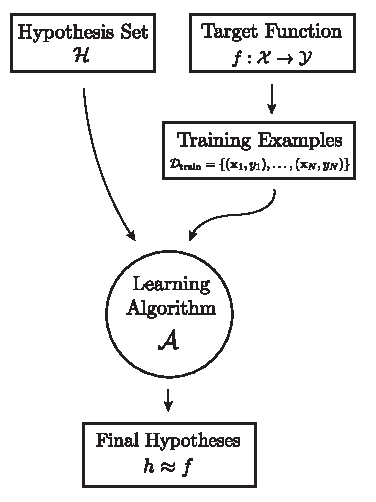
\includegraphics[width=0.99\textwidth, trim=5 5 10 5, clip]{figures/learning_problem/learning_problem.pdf}
  \caption[Overview of the learning problem.]
    {Schematic overview of the learning problem and how to find the optimal hypothesis $h^*$ to approximate $f$ given the training data $\mathcal{D}_\mathrm{train}$.
    }
  \label{fig:ml:learning_problem}
\end{marginfigure}

Without any loss of loss of generality let the focus for now be on classification. The goal is to find the underlying \q{true} function $f: \mathcal{X} \mapsto \mathcal{Y}$ that gives the correct label $y\in\mathcal{Y}$ for each observation $\vec{x}\in\mathcal{X}$. This function, however, is unknown and cannot perfectly be found. Although it is impossible to find $f$ it is possible to learn an approximation of it $h$ based on some training observations $\mathcal{D}_\mathrm{train} = \left \{(\vec{x}_1, y_1), \dots, \vec{x}_N, y_N) \right\}$. The optimal hypothesis, $h^*$, is chosen among a set of candidate hypotheses $\mathcal{H} = \left\{h_1, h_2, \ldots, h_M  \right\}$, and hopefully $h^*$ will be a good approximation of $f$, $h^* \approx f$. A schematic overview of this process can be seen in Figure~\ref{fig:ml:learning_problem}. 

How can one make sure that $h^*$ really is a good approximation of $f$? That is where Statistical learning theory comes into play. From a statistical standpoint we are interested in modelling the unknown joint probability $P(\vec{x}, y)$ over $\mathcal{X}$ and $\mathcal{Y}$. We assume that $\mathcal{D}_\mathrm{train}$ is independent and identically distributed (\emph{iid})\sidenote{This is one of the two key assumptions of statistical learning theory, the other being that future events are coming from the same distrubution as the one that generated the past events. These assumptions are sometimes called the PAC assumtions where PAC is an abbreviation for Probably, Approximatelly Correct.} from $P(\vec{x}, y)$ and thus want to find the hypothesis whose predictions $h(\vec{x})=\hat{y}$ matches the conditional probability distribution $P(y|\vec{x})$ as best as possible. 

To quantify the statement \q{as best as possible} in the previous paragraph we define the loss function $\ell$ which measures the loss for predicting $\hat{y}$ instead of $y$: $\ell(\hat{y}, y) = \ell(h(\vec{x}), y) \in \mathbb{R}^+$. Given $\ell$ we now introduce the method of (empirical) risk minimization \citep{vapnikPrinciplesRiskMinimization1991} and the expected loss\sidenote{Also called expected error or the out-of-sample error.}:
\begin{equation} 
  \label{eq:L}
  L(h) = \mathbb{E} \left[\ell(h(\vec{x}), y) \right] = \int \ell(h(\vec{x}), y)  \, dP(\vec{x}, y).
  \end{equation}
The optimal hypotheses $h^*$ is the hypothesis which minimizes the expected loss $L(h)$. However, the joint probability distribution $P(\vec{x}, y)$ is unknown and we are thus left with the empirical loss\sidenote{Also called empirical error.} of $h$ on $\mathcal{D}$:
\begin{equation}
  \label{eq:L_hat}
  \hat{L}(h, S) = \frac{1}{N} \sum_{i=1}^{N} \ell(h(\vec{x}_i), y_i), % \equiv \mathcal{L} 
\end{equation}
which is an approximation of $L(h)$ based on the training data available. 
% In the remainder of the text $\hat{L}(h, S)$ and $\mathcal{L}$ will be used interchangeably. 
Now the optimal hypothesis $h^*$ can defined:
\begin{equation}
  h^* = \argmin_{h\in\mathcal{H}} \hat{L}(h, S).
\end{equation}

\section{Generalization Bound}
\label{sec:generalization_bound}
In \autoref{sec:ml:supervised_learning} the method of selecting the optimal hypothesis $h^*$ out of the total set of candidate hypothesis $\mathcal{H}$ was sketched. However, there is still no guarantee that $h^*$ will work well, that is to say that the \emph{generalization error} $G(h)$ might be big:
\begin{equation}
  G(h) = \hat{L}(h, S) - L(h).
\end{equation}
The generalization error is thus the difference between the expected error $L(h)$ and the empirical error $\hat{L}(h, S)$. It describes the loss in performance of our chosen model compared to the optimal, yet hidden, model. Since $P(\vec{x}, y)$ is unknown, $G(h)$ cannot be computed, however, it is possible to bound this error using statistical learning theory. To do so, the union bound and Hoeffding's (one-sided) inequalities are introduced. 
\begin{lemma}[The Union Bound]
  For any finite or countably infinite sequence of events $E_1, E_2, \dots$ (not necessarily independent): 
  \begin{equation}
    \mathbb{P} \left\{\bigcup_{i \leq 1} E_i \right\} \leq \sum_{i \leq 1} \mathbb{P} \left\{E_i \right \}. 
  \end{equation}
\end{lemma}
The union bound, in simple terms, states that the probability of any one of $n$ events happening is less than or equal to the sum of the individual probabilities of the events happening. As an example, let $E_1=\{2, 4, 6\}$ be the event that a die rolls an even number and $E_2=\{4, 5, 6\}$ be the event that a die rolls a number larger than or equal to $4$. Then $\mathbb{P} \left\{E_1 \cup E_2 \right\} = \mathbb{P} \left\{ 2, 4, 5, 6 \right\} \leq \mathbb{P} \left\{E_1 \right \} + \mathbb{P} \left\{E_2 \right \} $. 
\begin{lemma}[The one-sided Hoeffding's inequalities]
  Let $Z_1, \dots, Z_n$ be independent random variables each belonging to the $[0, 1]$ interval such that $\mathbb{P}\left\{Z_i \in [0, 1] \right\} = 1$ and $\mathbb{E}[Z_i] = \mu$ for all i, then for every $\epsilon > 0$:
  \begin{equation}
    \mathbb{P} \left\{  \frac{1}{N}\sum_{i=1}^N Z_i - \mu \geq \epsilon \right\} \leq e^{-2n\epsilon^2} 
    \label{eq:hoeffding_onesided_a}
  \end{equation}
  and
  \begin{equation}
    \mathbb{P} \left\{ \mu - \frac{1}{N}\sum_{i=1}^N Z_i  \geq \epsilon \right\} \leq e^{-2n\epsilon^2}.
    \label{eq:hoeffding_onesided_b}
  \end{equation}
\end{lemma}
When using the union bound on equation \eqref{eq:hoeffding_onesided_a} and equation \eqref{eq:hoeffding_onesided_b} we arrive at Hoeffding's (two) sided inequality:
\begin{lemma}[The two-sided Hoeffding's inequality]
  \label{lemma:hoeffding}
  Let $Z_1, \dots, Z_n$ be independent random variables each belonging to the $[0, 1]$ interval such that $\mathbb{P}\left\{Z_i \in [0, 1] \right\} = 1$ and $\mathbb{E}[Z_i] = \mu$ for all i, then for every $\epsilon > 0$:
  \begin{equation}
    \mathbb{P} \left\{ \left| \frac{1}{N}\sum_{i=1}^n Z_i - \mu \right| \geq \epsilon \right\} \equiv \mathbb{P} \left\{ \left| \hat{\mu} - \mu \right| \geq \epsilon \right\} \leq 2 e^{-2N\epsilon^2},
    \label{eq:hoeffding_inequality}
  \end{equation}
  where we have defined the (empirical) average of $Z$ to be $\hat{\mu}$: $\hat{\mu}=\frac{1}{n}\sum_{i=1}^N Z_i $
\end{lemma}
Assuming that the loss $\ell(\hat{y}, y)$ is bounded in the $[0, 1]$ interval\sidenote{Which it is for classification, however, it can be extended in a similar fasion for regression.}, $\ell(\hat{y}, y) \in [0, 1]$ for all $\hat{y}, y$, we can bound the generalization error $G(h)$ by letting $Z_i = \ell(\hat{y}_i, y_i) = \ell(h(\vec{x}_i, y_i))$ be the loss of $h$ in sample $(\vec{x}_i, y_i)$. By comparing Lemma \ref{lemma:hoeffding} and equation \eqref{eq:L_hat} we see that $\hat{\mu} = \hat{L}(h, S)$, and similar for equation \eqref{eq:L}: $\mu = L(h)$. We then see that the generalization error is bounded:
\begin{equation}
  \label{eq:hoeffding_inequality_generalization_error}
  \mathbb{P} \left\{ \left| G(h) \right| \geq \epsilon \right\} = \mathbb{P} \left\{ \left| \hat{L}(h, S) - L(h) \right| \geq \epsilon \right\} \leq 2 e^{-2N\epsilon^2}.
\end{equation}
This equation provides a bound on the difference between the empirical loss and the expected loss. Say the probability of the generalization error being larger than $\epsilon = 0.1$ is needed for $N=100$ samples, we find that the this probability is $P=27\%$. The generalization bound  can be rewritten in terms of $\delta$:
\begin{equation}
  \delta = 2 e^{-2N\epsilon^2} \in (0, 1) \quad \Rightarrow \quad \epsilon = \sqrt{\frac{\ln \frac{2}{\delta}}{2N}} \quad \Rightarrow
\end{equation}
\begin{theorem}[Hoeffding's inequality for a single hypothesis]
  \label{theorem:hoeffding_single}
  Assume that $\ell$ if bounded in the $[0, 1]$ interval, then for a single hypothesis $h$ and any $\delta\in(0,1)$ we have:  
  \begin{equation}
    \label{eq:hoeffding_inequality_generalization_error_delta}
    \mathbb{P} \left\{ \left| \hat{L}(h, S) - L(h) \right| \geq \sqrt{\frac{\ln \frac{2}{\delta}}{2N}}  \right\} \leq \delta.
  \end{equation}
\end{theorem}
Equation \eqref{eq:hoeffding_inequality_generalization_error_delta} can be read as the probability of the generalization error being larger than $\sqrt{\frac{\ln \frac{2}{\delta}}{2N}}$ is $\delta$ or similarly that with probability greater than $1-\delta$:
\begin{equation}
  \label{eq:hoeffding_inequality_single_PAC}
  \left| \hat{L}(h, S) - L(h) \right| \leq \sqrt{\frac{\ln \frac{2}{\delta}}{2N}}.
\end{equation}
This is a powerful result relating the performance for a (fixed) hypothesis $h$ with the number of samples, $N$. We see that a higher $N$ yields a tighter bound on the generalization error, however, inversely\sidenote{Not to be understood as $1/x$ in this context.} related to on the certainty\sidenote{Technically the certainty of the model is $1-\delta$.} $\delta$ of this bound. 

There is a big assumption of this derivation although: that the hypothesis $h$ cannot depend on the sample $S$ and thus has to be chosen before seeing the data. We say that $h$ has to be \emph{fixed}. Of course the term machine learning indicates that some kind of learning is taking place: exactly as seen previously where we wanted to find the optimal hypotheses $h^*$ out of all the possible ones $\mathcal{H}$. For now assume that $\mathcal{H}$ is finite and consists of $M$ hypotheses: $|\mathcal{H}| = M$. We thus have $[h_1, h_2, \dots, h_M]$ hypotheses which we test simultaneously and where Hoeffding's inequality is true for each of them leading to the following theorem:
\begin{theorem}[Hoeffding's inequality for a finite set of hypotheses candidates]
  \label{theorem:hoeffding_finite}
  Assume that $\ell$ is bounded in the $[0, 1]$ interval and that $|\mathcal{H}| = M$. Then for any $\delta\in(0,1)$ we have:  
  \begin{equation}
    \label{eq:hoeffding_inequality_theorem_multiple}
    \mathbb{P} \left\{ \exists h \in \mathcal{H}: \left| \hat{L}(h, S) - L(h) \right| \geq \sqrt{\frac{\ln \frac{2M}{\delta}}{2N}}  \right\} \leq \delta.
  \end{equation}
\end{theorem}

\begin{proof}
  The proof begins by denoting $H_i$ as the event where: 
  \begin{equation*}
    \left| \hat{L}(h_i, S) - L(h_i) \right| \geq \sqrt{\frac{\ln \frac{2}{\delta'}}{2N}},
  \end{equation*}
   and then taking the union bound (the first inequality) followed by applying Hoeffding's inequality to each part in the sum (the second inequality): 
\begin{equation*}
  % \label{eq:hoeffding_inequality_generalization_error_delta}
  \begin{split}
    \mathbb{P} \Biggl\{ \exists h \in \mathcal{H}: \left| \hat{L}(h, S) - L(h) \right| &\geq \sqrt{\frac{\ln \frac{2}{\delta'}}{2N}}  \Biggr\} \\
    &= \mathbb{P} \left\{ \bigcup_{h \in \mathcal{H}} \left| \hat{L}(h, S) - L(h) \right| \geq \sqrt{\frac{\ln \frac{2}{\delta'}}{2N}}  \right\}  \\
    &\leq \sum_{h \in \mathcal{H}} \mathbb{P} \left\{\left| \hat{L}(h, S) - L(h) \right| \geq \sqrt{\frac{\ln \frac{2}{\delta'}}{2N}} \right\}  \\
    &\leq \sum_{h \in \mathcal{H}} \delta' \\
    &= M \delta'.
  \end{split}
\end{equation*}
By making the substitution $\delta = M \delta'$ we arrive at equation \eqref{eq:hoeffding_inequality_theorem_multiple}. 
\end{proof}

As we did in equation \eqref{eq:hoeffding_inequality_single_PAC}, equation \eqref{eq:hoeffding_inequality_theorem_multiple} can also be read as with probability greater than $1-\delta$ then for all $h\in\mathcal{H}$:
\begin{equation}
  \label{eq:hoeffding_inequality_multi_PAC}
  \left| \hat{L}(h, S) - L(h) \right| \leq \sqrt{\frac{\ln \frac{2M}{\delta}}{2N}}.
\end{equation}
This bound is looser than the one for only a single hypothesis by a factor $\ln M$, however, this holds for the optimal hypothesis $h^*$. 

\subsection{Generalization Bound for infinite hypotheses}
\label{subsec:generalization_bound_infinite}
Section \ref{sec:generalization_bound} dealt with the case of a single hypotheses $h$ and a finite set of candidate hypotheses $h\in\mathcal{H}, |\mathcal{H}| = M$. When $M$ goes towards $\infty$ the generalization bound goes to $\infty$ and the bound becomes useless. However, even simple models such as a linear classifier\sidenote{Also known as the perceptron. Often includes a constant offset $b$ as well which is omitted for brevity.} that predicts $\hat{y}=1$ when the dot product $\vec{w}^T\vec{x}$ is positive and $\hat{y}=0$ when it is negative has $|\mathcal{H}| = \infty$. Since there an infinite number of hypotheses $h(\vec{w})$, assuming we allow $\vec{w}$ to take any real values as is almost always the case, $\mathcal{H}$ is infinite. 

To solve this obvious problem with the Hoeffding inequality, we introduce\sidenote{For proof, see: \citet{abu-mostafaLearningData2012}} the Vapnik-Chervonenkis (VC) generalization bound. The VC-bound is based on the so-called VC-dimension of the hypothesis space $\mathcal{H}$: $d_\mathrm{VC}(\mathcal{H}) = d_\mathrm{VC}$. The VC-dimension is a measure of the complexity of the hypothesis space, the degrees of freedom of the model so to say. For example the VC-dimension of the $d$-dimensional linear classifier defined above\sidenote{In the general case when the offset $b$ is included: $d_\mathrm{VC}=d+1$.} is $d_\mathrm{VC}=d$ for $\{\vec{x}, \vec{w}\} \in \mathbb{R}^d$. 
\begin{theorem}[VC Generalization Bound]
  \label{theorem:hoeffding_finite}
  Let $\mathcal{H}$ be a hypotheses class with VC-dimension: $d_\mathrm{VC}(\mathcal{H}) = d_\mathrm{VC}$. Then with probability at least $1-\delta$: 
  \begin{equation}
    \label{eq:VC_bound}
    L(h) \leq \hat{L}(h, S) + \sqrt{ \frac{8}{N} \ln \left( \frac{4}{\delta} \left( \left(2N \right)^{d_\mathrm{VC}} + 1 \right)  \right)} .
  \end{equation}
\end{theorem}
Equation \eqref{eq:VC_bound} states that the out of sample error $L(h)$ is bounded from above by the empirical error $\hat{L}(h, S)$ and the $\sqrt{ \boldsymbol{\cdot}}$ which is related to the complexity of the hypothesis space $\mathcal{H}$, the number of samples $N$ and the certainty $\delta$. We will call this model complexity penalty $\Omega(N, \mathcal{H}, \delta)$:
\begin{equation}
  \Omega(N, \mathcal{H}, \delta) = \sqrt{ \frac{8}{N} \ln \left( \frac{4}{\delta} \left( \left(2N \right)^{d_\mathrm{VC}(\mathcal{H})} + 1 \right)  \right)}.
\end{equation}
As the hypothesis space complexity $d_\mathrm{VC}$ grows, the generalization bound loosens but it is more likely that $\mathcal{H}$ contains a strong hypothesis. This relationship is called the approximation-estimation or the  \emph{bias-variance} tradeoff. When the model is too simple to properly fit the complexity in the data it is called \emph{underfitting}\sidenote{Here the error from $\hat{L}(h, S)$ dominates.}, when the model is so complex that it starts fitting the inherent noise in the data it is called \emph{overfitting}\sidenote{Here the error from $\Omega(N, \mathcal{H}, \delta)$ dominates.}. The loss as a function of model complexity gives the characteristic curve illustrated in Figure~\ref{fig:ml:empirical_risk}. As the model complexity increases the training loss decreases. Initially also the validation loss decreases, but at some point the behavior of model on the validation set worsens and the loss increases; overfitting happens. 

\begin{marginfigure}
  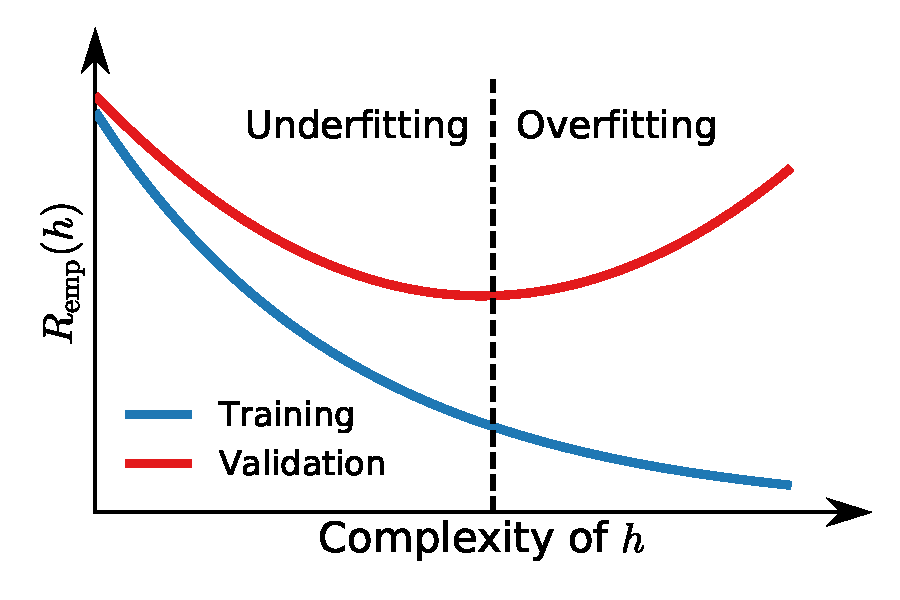
\includegraphics[width=0.98\textwidth]{figures/overfitting/overfitting_1.pdf}
  \caption[Approximation-Estimation tradeoff]
    {Illustration of the empirical loss as a function of model complexity. The \textcolor{blue}{training error} is shown in blue and \textcolor{red}{validation error} in red.
    }
  \label{fig:ml:empirical_risk}
\end{marginfigure}


\section{Avoiding overfitting}
\label{sec:ml:overfitting}
Avoiding overfitting is one of the most important issues in machine learning. By now, most modern machine learning algorithms have the inherent model complexity needed for overfitting and thus it has to be managed. Due to the importance of the issue, a number of different methods preventing or reducing overfitting exists. Most of them are not complementary of each other but can be taken advantage of in a combination. In this section model regularization will be introduced in \autoref{subsec:regularization}, cross validation in \autoref{subsec:cross_validation}, and early stopping in \autoref{subsec:early_stopping}. 

\subsection{Model Regularization}
\label{subsec:regularization}
One of the earliest methods developed for preventing overfitting was model regularization. A. N. Tikhonov \citep{tikhonovStabilityInverseProblems1943} was one of the first to describe this method in \num{1943}. In particular regularization was used to solve \emph{ill posed} linear regression problems. Regular linear regression problems refer to minimizing the residual sum of squares written in matrix form as:
\begin{equation}
  \begin{split}
    \hat{\bm{\beta}}_{\mathrm{LS}} = \argmin_{\bm{\beta}} \norm{\vec{y} - \vec{X} \bm{\beta} }_2^2 = \argmin_{\bm{\beta}} \norm{ \vec{y} - \vec{f}(\vec{X}) }_2^2 \\
    \vec{f}(\vec{X}) = \vec{X} \bm{\beta},
  \end{split}
\end{equation}
where $\vec{y}$ is vector of values we are trying to predict\sidenote{E.g. the prices of a collection of houses.}, $\vec{X}\in\mathbb{R}^{N\times M}$ is the matrix of input parameters such that each observation $\vec{x}_i \in \mathbb{R}^M$ is a $M$-dimensional vector stacked in $\vec{X}$ as rows with $N$ total observations, $\hat{\bm{\beta}}_{\mathrm{LS}}$ is the vector of unknown coefficients\sidenote{Here excluding the constant offset $\beta_0$ which can be included trivially.} of the linear least squares (LS) model $\vec{f}$, and $\norm{ \bm{\cdot} }_2$ is the normal Euclidean norm. In general, the $p$-norm is defined as:
\begin{equation}
  \norm{\vec{x}}_p = \left( \sum_{i=1}^N \abs{x_i}^p \right)^{1/p}.
\end{equation}
Differentiating the objective $\norm{\vec{y} - \vec{X} \bm{\beta} }_2^2$ with respect to (w.r.t.) $\bm{\beta}$ and setting the derivative equal to $0$ to find the minimum\sidenote{When checking the double derivative wrt. $\bm{\beta}$ it is seen that this really is a minimum and not a maximum (or saddle point).} yields the solution for $\bm{\beta}$:
\begin{equation}
  \begin{split}
    \frac{\partial}{\partial \bm{\beta}} \norm{\vec{y} - \vec{X} \bm{\beta} }_2^2 = -2 \vec{X}^T \left( \vec{y} - \vec{X} \bm{\beta} \right) = 0  \Rightarrow \\
    \vec{X}^T \vec{y} - \vec{X}^T \vec{X} \bm{\beta} \Rightarrow \\
    \hat{\bm{\beta}}_{\mathrm{LS}} =  \left( \vec{X}^T \vec{X} \right)^{-1} \vec{X}^T \vec{y}.
  \end{split}
\end{equation}
However, this solution for $\hat{\bm{\beta}}_{\mathrm{LS}}$ is only valid when $\vec{X}^T \vec{X}$ is invertible, i.e. $\vec{X}$ has to be full rank \citep{hastieElementsStatisticalLearning2009}. If this is not the case, the problem is said to be ill posed. Tikhonov solved this problem by adding an extra term to the minimization problem, which we will call $\Omega$ for simplicity. For a specific choice of $\Omega$, one gets:
\begin{equation}
  \label{eq:l2_norm}
  \hat{\bm{\beta}}_{\mathrm{L_2}} = \argmin_{\bm{\beta}} \left \{\norm{ \vec{y} - \vec{f}(\vec{X}) }_2^2 + \lambda \norm{ \bm{\beta} }^2_2 \right \},
\end{equation}
where $\lambda \geq 0$ is the regularization strength. This is the so-called $L_2$-regularization, also known as ridge regression for linear problems. For ridge regression\sidenote{Here $\hat{\bm{\beta}}_{\mathrm{L_2}}$ is the solution for any general function $\vec{f}$ and $\hat{\bm{\beta}}_{\mathrm{ridge}}$ is the specific solution for a linear function $\vec{f}$, where linear is w.r.t. to the model parameters $\bm{\beta}$.} the corresponding solution for $\bm{\beta}$ is:
\begin{equation}
  \label{eq:l2_norm_linear}
  \hat{\bm{\beta}}_{\mathrm{ridge}} =  \left( \vec{X}^T \vec{X} + \lambda \vec{I} \right)^{-1} \vec{X}^T \vec{y},
\end{equation}
where $\vec{I}$ is the identity matrix\sidenote{The $\lambda \vec{I}$ in equation \eqref{eq:l2_norm_linear} also acts as a conditioner on the problem in the sense that it reduces the condition number of the matrix to be inverted turning the ill-posed problem to a well-behaved one.}. This extra term, $\Omega =  \lambda \norm{ \bm{\beta} }^2_2$, acts as a shrinkage factor on the coefficients of $\bm{\beta}$. Looking at equation \eqref{eq:l2_norm}, we see that this is the Lagrangian form of the equivalent problem: 
\begin{equation}
  % \label{eq:ml:constrained_minimization_L2}
  \begin{split}
    \hat{\bm{\beta}}_{\mathrm{L_2}} = \argmin_{\bm{\beta}} \norm{ \vec{y} - \vec{f}(\vec{X}) }_2^2 \\
    \mathrm{subject~to:} \quad \sum_{i=1}^N \beta_i^2 = \norm{\bm{\beta}}^2_2 \leq t,
  \end{split}
  \label{eq:l2_norm_non_lagrangian}
\end{equation}

for some $t \geq 0$ with a one-to-one mapping between $\lambda$ and $t$. We thus see that $L_2$ regularizes the coefficients of $\bm{\beta}$ to have some maximal norm. The effect of the regularization is controlled by $\lambda$, where $\hat{\bm{\beta}}_{\mathrm{L_2}} \rightarrow \hat{\bm{\beta}}_{\mathrm{LS}}$ for $\lambda \rightarrow 0$ and $\hat{\bm{\beta}}_{\mathrm{L_2}} \rightarrow \vec{0}$ for $\lambda \rightarrow \infty$. An example of this can be seen in Figure~\ref{fig:ml:regularization_ridge}. 
\begin{marginfigure}
  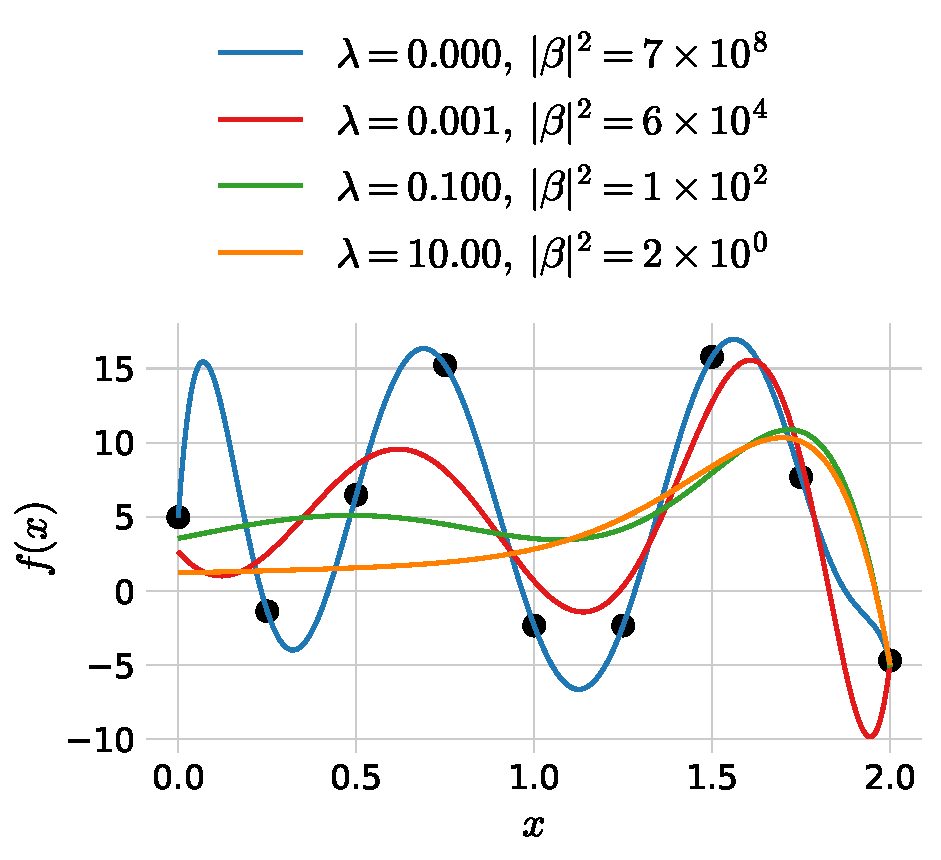
\includegraphics[width=0.99\textwidth, trim=5 5 5 5, clip]{figures/ridge_regression/ridge.pdf}
  \caption[Regularization Effect]
    {Effect of tuning the regularization strength $\lambda$ in ridge regression.
    }
  \label{fig:ml:regularization_ridge}
\end{marginfigure}
Here $N=9$ datapoints were randomly generated such that the $x$-values are evenly spaced from \num{0} to \num{1} and $y \sim \mathcal{N}(\mu=0, \sigma=10)$. They were then fit with a \num{9}-order polynomial by minimizing equation \eqref{eq:l2_norm} for different values of $\lambda$. Here we see the regularizing effect of $\lambda$, going from $\lambda=0$ in blue which fits all points\sidenote{Since the order of the polynomial is the same as the number of datapoints.} with a high degree of variance and a wildly oscillatory pattern to $\lambda=10$ in orange which is mostly flat in most of the interval. Also note in the legend how the norm of the fit parameters also decrease with $\lambda$ as expected. This is a great example of the \emph{bias-variance} tradeoff mentioned in \autoref{subsec:generalization_bound_infinite}, where bias refers the error the model makes when it is not advanced enough to fit the overall trend in the data (underfitting) and variance refers to the error the model makes when it starts to fit spurious noisy fluctuations in the training set which are not present in the validation set (overfitting). In this example $\lambda=0$ is clearly overfitting the data whereas $\lambda=10$ is an example of underfitting. 

\begin{marginfigure}
  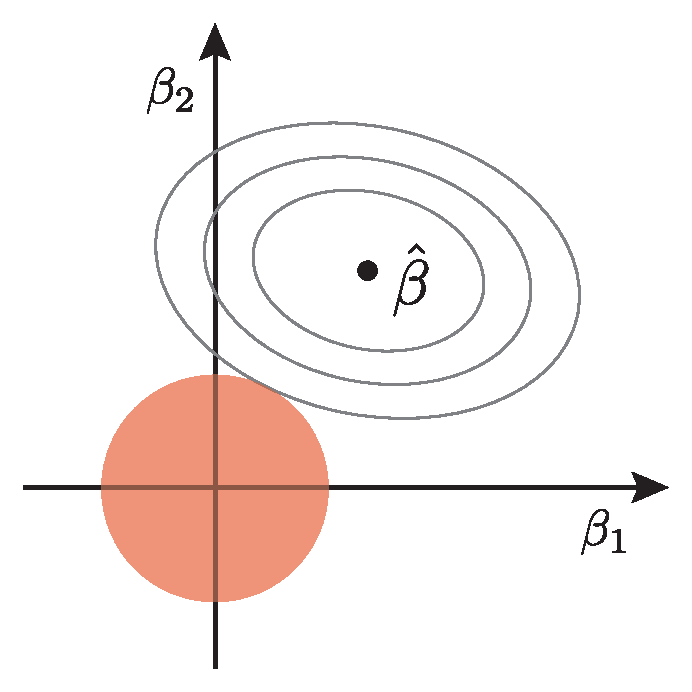
\includegraphics[width=0.7\textwidth]{figures/ridge_lasso_sparse/ridge.pdf}
  \caption[Regularization Effect of $L_2$ ]
    {Sketch of the minimization problem defined in equation \eqref{eq:l2_norm_non_lagrangian}, i.e. for a $L_2$-penalty. The \textcolor{red}{constrain region} shown in red is defined as $\beta_1^2 + \beta_2^2 \leq t$ for $L_2$ in $2D$-space and the contours of the unconstrained solution is shown with grey, dashed lines. 
    }
  \label{fig:ml:regularization_effect_ridge}
\end{marginfigure}
\begin{marginfigure}
  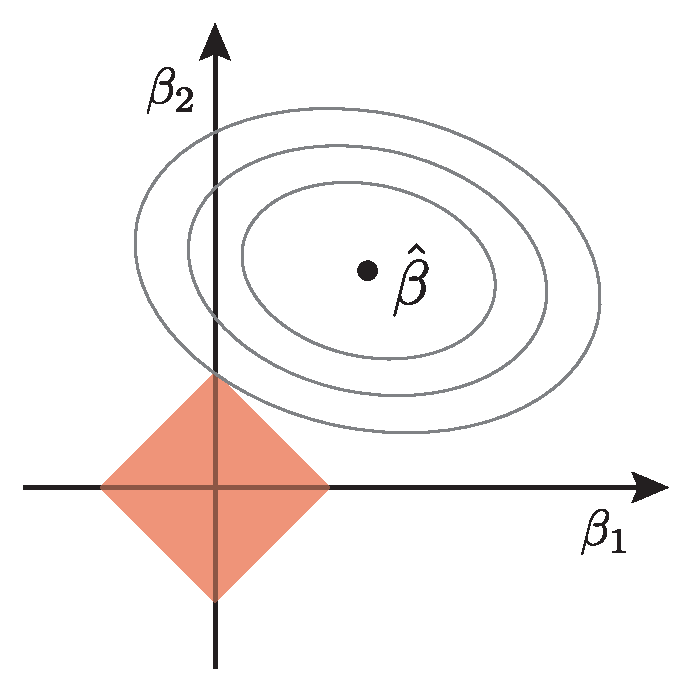
\includegraphics[width=0.7\textwidth]{figures/ridge_lasso_sparse/lasso.pdf}
  \caption[Regularization Effect of $L_1$]
    {Sketch of the similar minimization problem defined in Figure~\ref{fig:ml:regularization_effect_ridge} for the $L_1$-penalty. The \textcolor{red}{constrain region} shown in red is defined as $\abs{\beta_1} + \abs{\beta_2} \leq t$ for $L_1$ in $2D$-space and the contours of the unconstrained solution is shown with grey, dashed lines.
    }
  \label{fig:ml:regularization_effect_lasso}
\end{marginfigure} 

Other values of the regularization function $\Omega$ exists, for example the $L_1$-penalty:
\begin{equation}
  \Omega = \lambda \norm{\bm{\beta}}_1, 
\end{equation}
where the 1-norm, also known as Manhattan norm, is used. In the case of linear problems the $L_1$-penalty leads to Lasso regression introduced by \citet{tibshiraniRegressionShrinkageSelection1996} in \num{1996}. As with the $L_2$-penalty, the $L_1$-penalty also regularizes the coefficients of $\bm{\beta}$, however, this loss leads to sparse\sidenote{Meaning that a number of the $\beta_i$ coefficients are 0, the number depending on $\lambda$.} solutions. An illustration of this can be seen in Figure~\ref{fig:ml:regularization_effect_ridge} and Figure~\ref{fig:ml:regularization_effect_lasso} where the constraint regions of $\bm{\beta}$ os shown in red and the grey ellipses are the contours of the non-constrained problem. Notice how the intersection of the contour lines and the constrain region leads to $\beta_1 \neq 0, \beta_2 \neq 0$ for the $L_2$-penalty whereas it leads to the sparse solution $\beta_1=0, \beta_2 \neq 0$ for the $L_1$-penalty. This is a general pattern seen for $L_p$-penalties for $p \leq 1$.

Overall, model regularization is heavily used in modern machine learning algorithms. In general, the function or the so-called \emph{objective function} $\mathcal{L}$ they are trying to minimize is:
\begin{equation}
  \mathcal{L}(h) = \hat{L}(\ell, h, S) + \Omega(h)
\end{equation}
where $\hat{L}$ is the empirical loss and $\Omega$ is the regularization penalty. As can be seen from the above discussion, choosing the right value for the regularization strength is fundamental problem in model regularization. How to choose a suitable value for $\lambda$ is discussed in \autoref{subsec:cross_validation} and the choice of the training loss function $\ell$ in \autoref{sec:loss_function}. 

\subsection{Cross Validation}
\label{subsec:cross_validation}
In general we want to  be able to estimate the performance\sidenote{\q{Performance} is used here as the word for the general metric to be optimized for, no matter whether or not this metric should be maximized or minimized.} of the developed model. Since evaluation the model on the data it was already trained on would give a biased estimate of the performance, we need an unbiased method of doing so. The easiest way of doing so would be to set a fraction of the data aside, e.g. \SI{20}{\percent}, train on the remaining part and then evaluate the performance on the data set aside. Splitting the data up like this would provide us with a training (data)set and a test set in a $\num{80}:\num{20}$ ratio. This would then yield an unbiased performance estimate when evaluation the performance on the test set. 
However, if one then needed to compare two different models and choose the best one, as is often the case, this method would not work since we would choose the model with the best performance on the test set which can be seen as training on the test set and thus it has \q{tainted} the purity of the test set. To avoid this, an additional split is made such that we get a training set, a validation set, and a test set, where you often see a $\num{80}:\num{10}:\num{10}$ ratio. The two models can then be compared on the validation set and the performance of the chosen model can be estimated from the test set. 

\begin{marginfigure}
  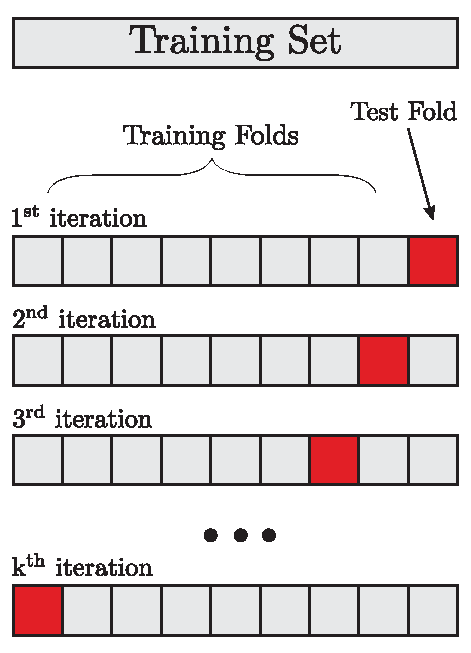
\includegraphics[width=0.98\textwidth, trim=5 5 5 5, clip]{figures/cross_validation/kfold.pdf}
  \caption[$k$-Fold Cross Validation]
    {$k$-fold cross validation. 
    }
  \label{fig:ml:cross_val_kfold}
\end{marginfigure} 

\begin{marginfigure}
  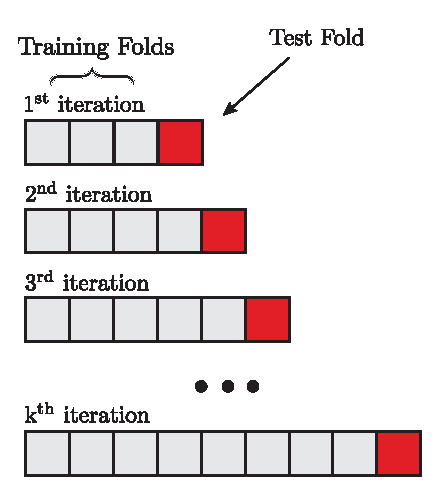
\includegraphics[width=0.98\textwidth, trim=10 10 10 10, clip]{figures/cross_validation/kfold_time.pdf}
  \caption[$k$-Fold Cross Validation for Time Series Data]
    {$k$-fold cross validation for time series data. 
    }
  \label{fig:ml:cross_val_kfold_time}
\end{marginfigure} 

This way of splitting up the data has some clear benefits and is thus also often used. There is a drawback, however, and that it that we are not fully utilizing a lot of the data in this way. Basically\SI{20}{\percent} of the data are only used to provide a single number of performance and does not necessarily allow an uncertainty or confidence interval of this measurement to calculated. Thus other methods of estimating model performance are developed where one of the most used and well-known are the $k$-fold cross validation (CV). Here the entire dataset are split up into $k$ chunks which are randomly drawn subsamples (without replacement). In the first iteration, the model is trained on the first $k-1$ subsamples and evaluated on the last $k$ subsample. In the second iteration the evaluation subsample is a new one. This process is continued $k$ times until all samples in the dataset have been trained and evaluated on \citep{hastieElementsStatisticalLearning2009}. For an illustration of this, see Figure~\ref{fig:ml:cross_val_kfold}. The process yields $k$ estimates of the performance of the model which can then be averaged to form a single performance number and the variability of the performance can even be gauged\sidenote{Special care has to be taken here since the $k$ different performance values are not independent.}. The disadvantage of $k$-fold CV is that the performance estimate is now slightly biased, however, this effect is generally very small. The biggest disadvantage is the computational burden related to doing $k$-fold CV where $k\gg 1$. A compromise often used in applied ML is $k=5$ which is also what is used in this project.  

Special care has to be taken when dealing with time series data. Here the problem of \q{data leakage} is often introduced inadvertently. Data leakage is when the model is exposed to information from the test set that it was not supposed to be exposed to. In the case of time series data, if the data is split by the usual $k$-fold CV, then each subsample contains events from all times and the model does not learn how to predict future events. To circumvent this problem, a special type of $k$-fold CV for time series data has to be used. Here all samples up to a specific time, eg. all houses sold before 2018, is used for training and then it is evaluated on the performance of samples after the event, e.g. houses sold in \num{2018}. For an illustration of this, see Figure~\ref{fig:ml:cross_val_kfold_time}.


\subsection{Early Stopping}
\label{subsec:early_stopping}
Most modern machine learning models are trained iteratively. This is the case for both (boosted) decision trees and neural networks, both of which are used in this project. Iteratively here means that the model starts off with an initial guess of the parameters of the model to learnt and then by looking at the data \q{learns} a new set of values for the parameters. The question then become: for how long should the model be allowed to continue training. 

This is a prime example of the bias-variance tradeoff. The model should be trained long enough to be able to capture the complexity inherent in the data but also should not train for so long that it starts to overfit the data. Even though Figure~\ref{fig:ml:empirical_risk} was just an illustration of the bias variance tradeoff, it is also something that is seen in real data and can taken advantage of through \emph{early stopping}. Early stopping is the process of monitoring the loss for training set and validation set $\mathcal{D}_\mathrm{train}$ and $\mathcal{D}_\mathrm{val}$. As mentioned in \autoref{subsec:cross_validation}, the model is only fitted on $\mathcal{D}_\mathrm{train}$ but the performance on $\mathcal{D}_\mathrm{val}$ is also measured. Whenever the validation loss starts to increase, the training of the model should be terminated. 

To avoid stopping just because of a single outlier due to noise that terminated the process, one often uses \emph{patience} in the early stopping process: if the loss has not decreased since the last minimum after \emph{patience} number of iterations, then terminate the process. Early stopping is thus an easy way of avoiding overfitting for iteratively trained models only requiring a validation set.  

\section{Loss functions}
\label{sec:loss_function}
How we evaluate the performance of a model is of course very important since it defines the metric for the problem; what is good and what is bad? Obviously this depends on whether or not we a dealing with a classification problem or a regression problem. Let us for know focus on the latter. Say that a house is estimated to cost \num{2} million DKK (\si{\Mkr}) but was sold for \SI{4}{\Mkr}. Compare this to an a house that was estimated to cost \SI{8}{\Mkr} but was sold for \SI{6}{\Mkr} In both cases the price was \SI{2}{\Mkr} wrong, but does this mean that both predictions are equally good? The first case was a factor of 2 off, whereas the second was only $25\%$ off. The first case underestimated the price whereas the second overestimated. 

As it should be clear by now the choice of loss function $\ell$ is of utmost importance. It is also not a problem that can be solved by computers, is problem-specific, and has to be defined manually. The choice of loss function is what is called a \emph{hyper parameter}, the optimization of which is further discussed in \autoref{sec:ml:hyperparameter_optimization}. The most common choice of loss function is by far the Squared Error (SE): 
\begin{equation}
  \ell_\mathrm{SE}(y, \hat{y}) = \left( y-\hat{y} \right)^2,
\end{equation}
where $y$ is the true value and $\hat{y}$ is the predicted one. Squared Error has the advantage that it is differentiable everywhere, an effect that is both needed for many statistical derivations but also a requirement for some machine learning models. The disadvantage is that it gives too much weight to outliers since every deviation away from the truth is squared. In contrast to this, there is the Absolute Error (AE) defined as:
\begin{equation}
  \ell_\mathrm{AE}(y, \hat{y})  = \abs{y-\hat{y} }.
\end{equation}

For AE, outliers have a lot smaller weight since it deals with the absolute value of the deviation and not the squared deviation. However, this comes at a price; AE is not differentiable at every point: at $y-\hat{y} = 0$ the derivative of the absolute value function is un-defined. Many functions have been invented trying to deal with these problems. For a more general discussion of loss functions, see e.g. Barron \citep{barronGeneralAdaptiveRobust2017}. Six different loss functions (for regression problems) have been investigated in this project. In addition to SE and AE also the LogCosh, Cauchy  \citep{barronGeneralAdaptiveRobust2017}, Welsch  \citep{barronGeneralAdaptiveRobust2017} and Fair  \citep{AllstateClaimsSeverity} loss functions are used:
\begin{equation}
  \begin{split}
    \ell_\mathrm{LogCosh}(y, \hat{y})  &= \log\left( \cosh\left( y-\hat{y} \right) \right) \\
    \ell_\mathrm{Cauchy}(y, \hat{y})  &= \log\left( \frac{1}{2} \left(\frac{y-\hat{y}}{c}\right)^2 + 1   \right) \\
    \ell_\mathrm{Welsch}(y, \hat{y})  &=  1 - \exp\left( - \frac{1}{2} \left(\frac{y-\hat{y}}{c}\right)^2  \right)\\
    \ell_\mathrm{Fair}(y, \hat{y})  &= c^2  \left( \frac{\abs{y-\hat{y}} }{c}  - \log \left(\frac{\abs{y-\hat{y}}}{c} +1 \right )   \right). 
  \end{split}
\end{equation}
The above loss functions share some similarities with AE, and in addition to this they are all (twice) differentiable functions. They are shown in Figure~\ref{fig:ml:objective_funcs}. They are shown for only positive values of $y-\hat{y}$ since they are symmetric in $y-\hat{y}$. Notice how SE quickly grows very large compared to the others. Absolute Error has a kink at $y-\hat{y}=0$ as the only one of the functions. Welsch is bounded in the interval $[0, 1)$. The derivative of both LogCosh and Fair goes toward $1$ when $y-\hat{y}$ goes towards $\infty$, whereas it goes to 0 for the Cauchy loss. A priori it is almost impossible to know which one of these loss functions performs best for a specific data set, so they have to be treated as hyper parameters. 

\begin{figure}
  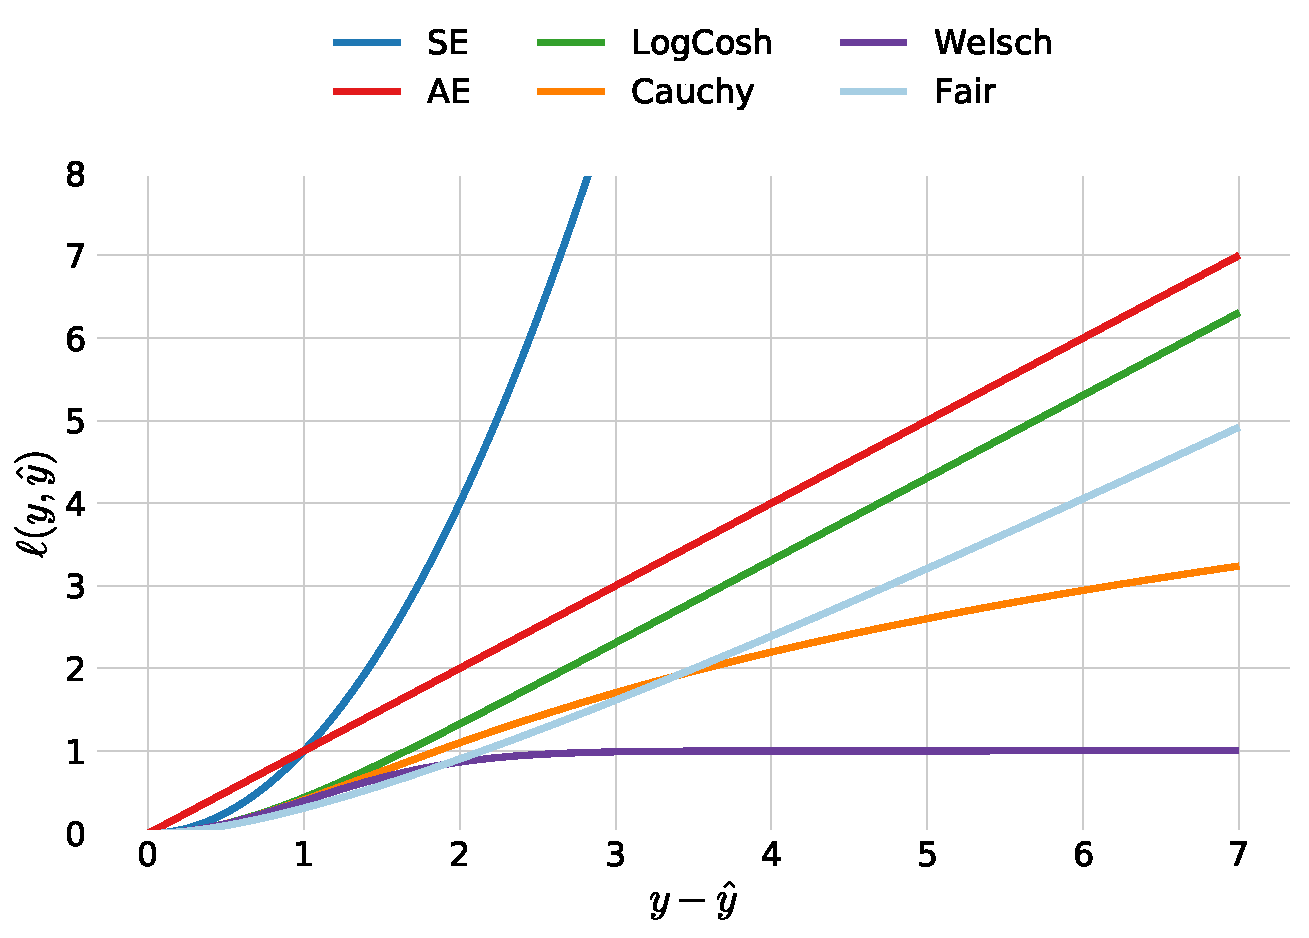
\includegraphics[width=0.9\textwidth]{figures/objective_functions/objective_functions.pdf}
  \caption[Comparison of different objective functions.]
    {Comparison of the the six loss functions SE, AE, LogCosh, Cauchy, Welsch, and Fair as a function of $y-\hat{y}$. In the plot \textcolor{blue}{SE} is shown in blue, \textcolor{red}{AE} in red, \textcolor{green}{LogCosh} in green, \textcolor{orange}{Cauchy} in orange, \textcolor{purple}{Welsch} in purple, and \textcolor{light-blue}{Fair} in light blue. For the Cauchy, Welsch, and Fair functions $c$ is set to 1. For a zoom in of the inner region 
    where $y-\hat{y}<2$ see \figref{fig:ml:objective_funcs_zoom}. All six graphs are symmetric in $y-\hat{y}$ which is why they are only shown for positive values of $y-\hat{y}$.
    }
  \label{fig:ml:objective_funcs}
\end{figure}

\begin{marginfigure}
  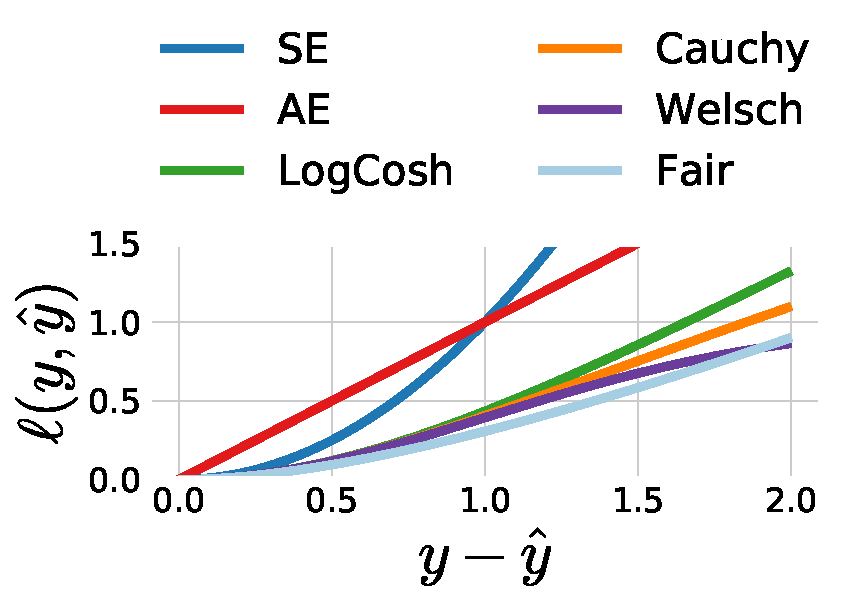
\includegraphics[width=0.98\textwidth]{figures/objective_functions/objective_functions_zoom.pdf}
  \caption[Comparison of different objective functions zoom in.]
    {Zoom in of \figref{fig:ml:objective_funcs}. 
    }
  \label{fig:ml:objective_funcs_zoom}
\end{marginfigure}

\subsection{Evaluation Function}
Since some machine learning models require an analytic expression for the derivative and second derivative, it not always possible to use a custom objective function if it is non-differentiable. The Area Under Curve (AUC) of the Receiver Operating Characteristic (ROC) is such a measure. Another example would be the width of the distribution of all $y_i-\hat{y}_i$. In this thesis this overall performance metric will be called the \emph{evaluation function} $f_\mathrm{eval}$ compared to the differentiable proxy for this function, the objective function. To sum up: the loss function $\ell(y, \hat{y})$ measures the loss for an individual prediction and the objective function $\mathcal{L}$ is the aggregated version of the individual losses. The objective function is assumed to be a good proxy for the evaluation function. 

For the loss functions defined in \autoref{sec:loss_function} the objective function is based on the mean of the individual losses:
\begin{equation}
  \mathcal{L} = \frac{1}{N} \sum_{i=1}^N \ell(y_i, \hat{y}_i) + \Omega. 
\end{equation}

\section{Decision Trees}
\label{sec:ml:decision_trees}

\begin{marginfigure}[-3cm]
  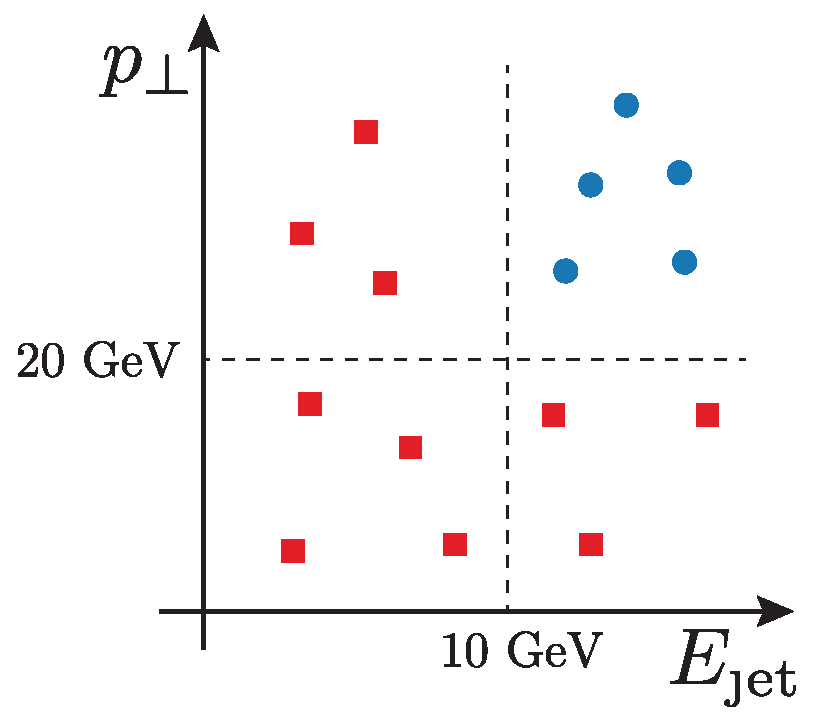
\includegraphics[width=0.99\textwidth, trim=10 10 10 10, clip]{figures/decision_tree/tree_example.pdf}%     without .tex extension
  % or use \input{mytikz}
  \caption[Decision Tree Cuts In Feature Space]{Illustration of the cuts a decision tree model make for \textcolor{blue}{signal} in blue circles and \textcolor{red}{background} in red squares. This is an visualization in the feature space of the decision tree seen in Figure~\ref{fig:ml:decision_tree}.}
  \label{fig:ml:decision_tree_feature_space}
\end{marginfigure}

Decision Trees are a simple machine learning method that works by partitioning the feature space into smaller subspaces, high-dimensional rectangles basically, and then fit each subspace with a constant for regression problems or a single label for classification problems \citep{hastieElementsStatisticalLearning2009}. A simple example of this can be seen in Figure~\ref{fig:ml:decision_tree_feature_space} and Figure~\ref{fig:ml:decision_tree}. In the first figure we see an illustration of how the signal and background distributions look in the 2D feature space. The dashed lines in the figure indicate the cuts made by the decision tree (DT), cuts which are shown on the second figure as a typical DT plot. 
\begin{figure}
  \centering
  \includestandalone[width=0.6\textwidth]{figures/decision_tree/decision_tree}%     without .tex extension
  % or use \input{mytikz}
  \caption[Decision Tree]{
    Illustration of a simple decision tree. Here the tree partitions the input feature space consisting of the two variables $p_\perp$ and $E_\mathrm{jet}$ into two categories; either signal or background. A visualization of the cuts in the feature space can be seen in Figure~\ref{fig:ml:decision_tree_feature_space}.
  }
  \label{fig:ml:decision_tree}
\end{figure}
Here the first \q{box} is called the \emph{root} of the tree, any subsequent boxes are \emph{nodes} except the final ones that are not split any further which are \emph{leaves}.

At first the DT partitions the space according the the value of the transverse momentum\sidenote{All units in this project are in natural units such that both momentum and energy are in units of \si{\eV}.} $p_\perp$: if it is lower than (or equal to) \SI{20}{\GeV} then it classified as background. If the value is higher than \SI{20}{\GeV} then an extra split is made, this time on the energy of the jet $E_\mathrm{jet}$: if it is higher than \SI{10}{\GeV} it is classified as signal and otherwise as background. Training a DT on this data allows us to predict a new unseen event $(p_\perp, E_\mathrm{jet}) = (\SI{24}{\GeV},\SI{11}{\GeV})$ to be a signal-like event. This DT is said to be a shallow tree since it only has a depth of \num{2}. The maximum depth allowed for the model is an important hyperparameter since it clearly controls under- and overfitting by changing how many cuts and partitions in the feature space are allowed; the deeper the tree, the more complex the model becomes. Single DTs are very prone to overfitting\sidenote{With a solution to this problem given in \autoref{subsec:ml:multiple_decision_trees}.}, however, they are also extremely inspectable. They are even referred to as \q{white-box models} compared to black-box models such as neural networks. For a more thorough introduction to decision trees and how they are internally optimized (for finding the best cut values), see \citet{hastieElementsStatisticalLearning2009}. 

\subsection{Ensembles of Decision Trees}
\label{subsec:ml:multiple_decision_trees}
Single decision trees are prone to overfitting and generally suffer from high variance. Today especially two different methods exist to alleviate these problems: Random Forests (RFs) and Boosted Decision Trees (BDTs). Both methods are examples of so-called ensemble methods where a finite set of ML methods are combined into a single model. Typically ensemble methods are based on \emph{weak learners}: simple, often fast, methods that individually show relatively poor generalization performance typically due to variance. 

\subsubsection{Random Forests}
\label{subsubsec:ml:random_forest}
Random Forests were first introduced in 2001 by \citet{breimanRandomForests2001}. Random Forests are a collection of $B$ decision trees where each tree is trained on bootstrapped versions of the training data and the average\sidenote{In case of classification, it is the majority vote which is taken.} the individual trees' predictions $T_b$: 
\begin{equation}
  f_\mathrm{RF}(\vec{x}) = \hat{y}_\mathrm{RF} = \frac{1}{B}  \sum_{b=1}^B T_b(\vec{x}).
\end{equation}
The method of making artificial extra samples and training on them is in general called bootstrap aggregation or \emph{bagging}\autocite{hastieElementsStatisticalLearning2009}. It works by averaging out noisy estimates of the individual models hence reducing variance. 
\begin{theorem}[Variance of average of correlated i.d. variables]
  Given $B$ identically distributed (but not necessarily independent) variables each with variance $\sigma^2$ and positive pairwise correlation $\rho$, the variance of the average is:
  \begin{equation}
    \label{eq:ml:variance_of_correlated_variables}
    \mathrm{Var}(\bar{\mu}_B) = \frac{1-\rho}{B} \sigma^2 + \rho \sigma^2,
  \end{equation}
  where $\bar{\mu}_B$ is the average of the i.d. variables \autocite{hastieElementsStatisticalLearning2009}. % XXX myabe write proof here myself: https://stats.stackexchange.com/questions/320083/calculating-the-variance-of-the-average-of-b-dependent-random-variable
\end{theorem}
Equation \eqref{eq:ml:variance_of_correlated_variables} is the main idea behind RFs. As the number of trees $B$ in the forest increases, the first term goes towards zero. Thus, the more the correlation $\rho$ between the individual trees is reduced, the more the variance is reduced (which is the main problem in the case of DTs to begin with). 

In addition to training the trees on bagged samples, one more technique is used to further decrease the correlation between the individual trees: each bootstrapped sample of the dataset not only contains a only subset of the observations (rows), but also only a subset of the variables (columns)\sidenote{Throughout this project all data is assumed to be \emph{tidy data} unless otherwise explicitly mentioned. Tidy data was a concept formalized in 2003 by \citet{JSSv059i10} which basically states that each variable forms a columns, each observation forms a row, and that each type of observation unit forms a table. This also means that the term variable and column will be used interchangeable (together with \emph{feature}), and likewise with observation and row.}. This called columns subsampling (in contrast to row subsampling).

% Until very recently RF has suffered from the lack of a fast, optimized implementation in Python that could deal with big data sets. 

\subsubsection{Boosted Decision Trees}
\label{subsubsec:ml:boosted_decision_trees}
In the overall family of ensemble models, \emph{boosting} might be the most successful of them all where especially the specific algorithm called XGBoost \autocite{chenXGBoostScalableTree2016} revolutionized the ML world by winning numerous Kaggle\sidenote{XXX \TODO} competitions \autocite{DmlcXgboost} including the Higgs Machine Learning competition in \num{2014} \autocite{HEPMeetsML}. 

Boosting is the process of sequentially applying weak learner models to repeatedly modified versions of data \autocite{hastieElementsStatisticalLearning2009}. In an iterative fashion this combines many weak learners into a single strong learner. The final prediction is thus a weighted sum over the $M$ different weak learners $F_m$: 
\begin{equation}
  f_\mathrm{BDT}(\vec{x}) = F(\vec{x}) = \sum_{m=1}^M \alpha_m F_m(\vec{x})
\end{equation}
Boosting thus works by reducing both bias and variance since it iteratively fits weak learners. The variance is not reduced as much as for RFs since the weak learners are more correlated, however, their bias is lower. 

The term gradient boosting comes from the observation that repeatedly minimizing the residuals of the current model is similar to minimizing the gradient of the loss function for a specific choice of the loss function.

Imagine that we start off with an imperfect model $F_m(x)=\hat{y}$. In boosting we want the next iteration to be a better model than the previous one, so image that the perfect addition to the model that we needed to make was $h(x)$. For it to be perfect, the following would have to be true:
\begin{equation}
  \label{eq:ml:boosted_decision_trees_residual}
  F_{m+1}(x) = F_m(x) + h(x) = y \Leftrightarrow h(x) = y - F_m(x).
\end{equation}
The r.h.s. is the residual of the model, so at each stage the model is trying to fit the residuals of the current iteration of model. The \q{gradient} in \q{gradient boosting} comes from the following. Assume the loss function: $L(y, F_m(x)) = \frac{1}{2}  (y-F_m(x))^2$. The gradient of the loss w.r.t. to $F_m(x)$ is:
\begin{equation}
  \frac{\partial L(y, F_m(x))}{\partial F_m(x)} = F_m(x) - y. 
\end{equation}
This is exactly the negative of the r.h.s. of equation \eqref{eq:ml:boosted_decision_trees_residual}. Instead of looking at the model as trying to minimize the residual at each iteration, it can instead be generalized as trying to fit the negative gradients of the loss function:
\begin{equation}
  h(x) = - \frac{\partial L}{\partial F_m}.
\end{equation}
We thus end up with the following iterative model which is basically a \emph{gradient descent} algorithm.
\begin{equation}
  F_{m+1}(x) = F_m(x) + h(x) = F_m - \frac{\partial L}{\partial F_m}.
\end{equation}


AdaBoost \autocite{freundDesiciontheoreticGeneralizationOnline1995} was the first major algorithm to make use of boosting. It was seen as a way of iteratively giving wrongly predicted observations higher weight, however, this is just a result of a \q{lucky} choice of loss function\sidenote{Exponential loss for classification.} which was not realized until much later. AdaBoost could be used with many different weak learners, however mostly DTs were used to form BDTs. XGBoost \autocite{chenXGBoostScalableTree2016} is a fast, computationally efficient implementation of gradient boosting with DTs as base learners. It implements several model regularization techniques which makes it less prone to overfitting than other BDTs. In 2017 Microsoft released the competitor to XGBoost called LightGBM \autocite{keLightGBMHighlyEfficient2017}. In comparison to XGBoost, LightGBM implements some extra binning and categorical assumptions that greatly speeds up the fitting process. 

\section{Hyperparamater Optimization}
\label{sec:ml:hyperparameter_optimization}
By now linear models with $L_1$ and $L_2$ regularization have been introduced along with decision trees (DTs), random forests (RFs) and gradient boosted trees (GBTs). All of these ML models tries to optimize their parameters according to some objective function. In addition to the parameters of the model, each one has a specific set of \emph{hyperparameters} that cannot directly be optimized in internal optimization process. This could be amount of regularization $\lambda$ for linear models, the maximum tree depth for DTs, the number of trees for RFs, or the column (or row) subsampling fraction for BTDs. 

In general we say that we have the ML model $\mathcal{A}$ with $K$ hyperparameters. Each of these hyperparameters have a domain $\Lambda_n$. The domain can be either real numbers $\Lambda_k \in \mathbb{R}$, integers $\Lambda_k \in \mathbb{Z}$, binary $\Lambda_k \in \{0, 1\}$, or categorical\sidenote{Could e.g. be the choice of loss function.}. We define the hyperparameter configuration space as: $\bm{\Lambda} = \Lambda_1 \times \Lambda_2 \times \dots \times \Lambda_K$. Within this space we are searching for a vector of hyperparameters $\bm{\lambda} \in \bm{\Lambda}$ which defines the optimal model $\mathcal{A}_{\bm{\lambda}^*}$. Here the optimal model is the defined as the model which gives the best generalization performance according to some evaluation function. The goal of finding the best hyperparameter $\bm{\lambda^*}$ is known as \emph{hyperparameter optimization} (HPO.)

The first naive approach would simply to manually\sidenote{Also known as jokingly as \q{Grad Student Descent}.} try out different combinations of $\bm{\lambda}$ and see performance on the validation set\sidenote{Remember only to use the test set on the final model!}. This is of course too cumbersome for advanced ML models, but it should be noted that it is a good place to start. In \autoref{subsec:ml:grid_search} the HPO method called Grid Search is introduced which is further generalized and optimized in \autoref{subsec:ml:random_search} with Random Search. Both these methods are easily parallelizable since they do not have any inherent history in its guesses. This is in contrary to Bayesian Optimization introduced in \autoref{subsec:ml:bayesian_optimization} which allows for \q{smart} guesses.

\subsection{Grid Search}
\label{subsec:ml:grid_search}

Grid Seach (GS) is a HPO method also known as full factorial design. It is called this because it tries out all possible combinations of the hyperparameter configuration space: the so-called cartesian product of $\bm{\Lambda}$. Imagine a 2D space where the two domains are respectively $x=\{1, 2, 3\}$ and $y=\{1, 2, 3,4\}$. Then GS runs through all \num{12} combinations of these two sets: 

\begin{marginfigure}
  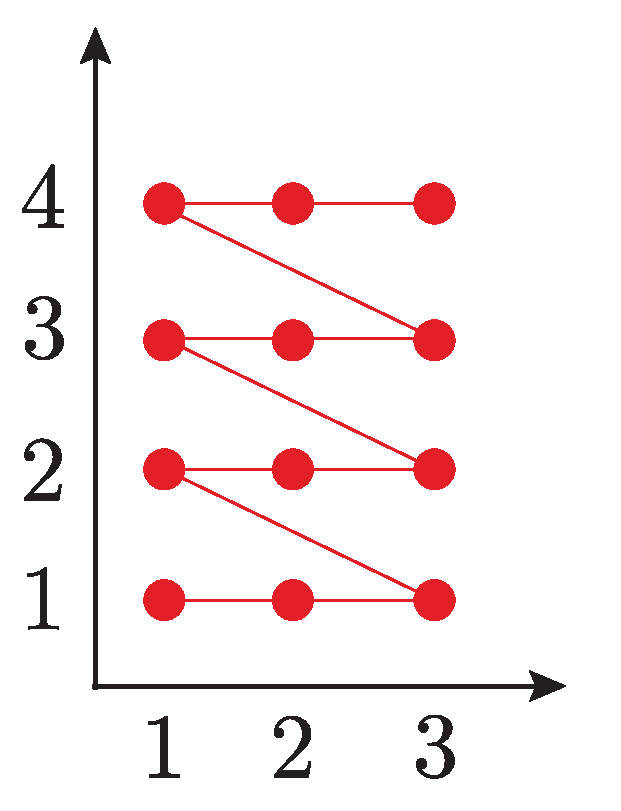
\includegraphics[width=0.8\textwidth]{figures/gridsearch/grid.pdf}
  \caption[Grid Search]{Visualization of grid search run on the two hyperparameters $x$ and why $y$ with the domains $x=\{1, 2, 3\}$ and $y=\{1, 2, 3,4\}$.}
  \label{fig:ml:gridsearch}
\end{marginfigure}

\begin{equation}
  \{(1, 1), (1, 2), \dots, (x_i, y_i), \dots, (3, 4)\},
\end{equation}
as visualized in Figure~\ref{fig:ml:gridsearch}. The advantage of GS is that it is an exhaustive search over all combinations\sidenote{Note that the user has to provide the values for each hyperparamater to be tried out manually.} of hyperparameters, however, the total number of combinations grows exponentially and GS as a method thus suffers the curse of dimensionality\sidenote{Not the dimensionality of the input feature space, but of the hyperparameter configuration space.}.



\subsection{Random Search}
\label{subsec:ml:random_search}

To circumvent the problems of grid search, \citet{bergstraRandomSearchHyperparameter2012} developed the Random Search (RS) algorithm in 2012. Regarding the effect of the curse of dimensionality on grid search they wrote: \emph{``This failure of grid search is the rule rather than the exception in high dimensional hyper-parameter optimization''} \citep{bergstraRandomSearchHyperparameter2012}. Instead of searching through all possible values of $\bm{\lambda}$ like in GS, RS makes $B$ runs where each $\bm{\lambda}_i$ is given by:
\begin{equation}
  \label{eq:ml:random_search}
  \bm{\lambda}_i \sim \sum_{j=1}^K  \mathrm{PDF}_j(\Lambda_j) \cdot \bm{\hat{e}}_j  .
\end{equation}
Equation \eqref{eq:ml:random_search} should be understood in the following way. For each hyperparameter draw a random number from a user-defined Probability Density Function (PDF) and then let $\bm{\lambda}$ be the vector of those $N$ random numbers. In a 2D-space $\bm{\lambda}_i$ could thus be: 
\begin{align}
  \bm{\lambda}_i \sim &= \begin{bmatrix}
      \mathcal{N}(100, 4) \\
      \mathcal{U}(0, 1)
       \end{bmatrix},
\end{align}
where $\mathcal{N}(100, 2)$ is normal (Gaussian) distribution with mean $\mu=100$ and standard deviation $\sigma^2=4$ and $\mathcal{U}(0, 1)$ is the uniform distribution in the interval $[0, 1]$. Of course the PDF can be a PMF in the case of discrete hyperparameter domains.

\begin{marginfigure}
  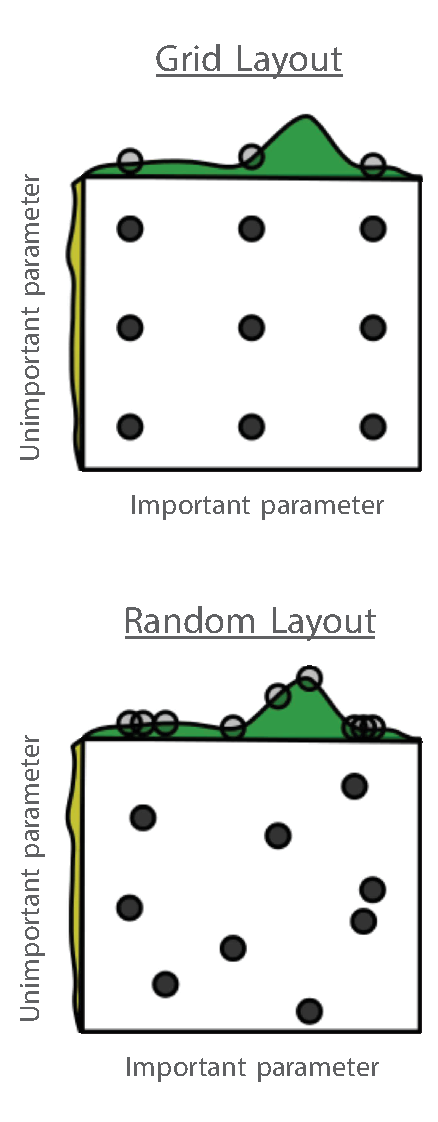
\includegraphics[width=0.8\textwidth]{figures/randomsearch/random.pdf}
  \caption[Random Search]{Visualization of the difference between grid search and random search. Adapted from \citet{bergstraRandomSearchHyperparameter2012}.}
  \label{fig:ml:random_search}
\end{marginfigure}

The reason why random search is so powerful is not only because the number of function evaluations $B$ is easily tunable\sidenote{Compared to grid search which tries \emph{all} possible combinations.}, but also due to the fact that often some hyperparameter dimensions are more important than other. Even though the hyperparameter configuration space $\bm{\Lambda}$  might be high-dimensional, it often exhibits \emph{low effective dimensionality} \autocite{bergstraRandomSearchHyperparameter2012}. In the simplest 2D-case this can be written as the following example. Imagine that we want to maximize some evaluation function, e.g. accuracy of the predictions, and the model depends on the two independent hyperparameters $x$ and $y$: $f(x, y)$. In this example assume that $f$ is almost insensitive to $y$ and thus has an effective dimensionality of 1. Then $f(x,y) = g(x) + h(y) \approx g(x)$. For a visualization of this example, see Figure~\ref{fig:ml:random_search}.

Here GS is run with a grid of $3\times3 = 9$ points and RS is similarly run with 9 points drawn from uniform PDFs in the same interval. It easy to see that when the hyperparameter configuration space has a lower effective dimensionality than the actual dimensionality RS is far better at probing the space due to the projections into the sensitive dimensions cover more of these axes than for GS. In general in ML the hyperparameter configuration space has lower effective dimension than its actual dimension, but the different hyperparameters matter in different datasets

In general only a fraction of all hyperparameters matter for any dataset but different hyperparameters matter in different datasets and thus generally RS performs as well as GS or better \autocite{bergstraRandomSearchHyperparameter2012}. 

Note that RS can be seen as a generalization of GS, where GS is the specific example of RS if one uses a multidimensional hypergeometric distribution as PDF where the PDF is reevaluated after each run. 

\subsection{Bayesian Optimization}
\label{subsec:ml:bayesian_optimization}
When optimizing the hyperparameters it often takes a lot of time to evaluate the individual hyperparameters. Remember, that each evaluation consists of fitting $\mathcal{A}_{\bm{\lambda}}$ to the training data and then measure the performance on the validation set. Fitting the model on the training set can often take minutes, if not hours. This process is even slower when using cross validation. The idea behind Bayesian Optimization is that when the ML model, or any other black box function, is expensive\sidenote{With respect to time.} to evaluate then \q{smart} guesses are worth spending a bit of time on developing. The hope is that the time taken to come up with smart guesses is negligible compared to the overall function evaluation time. This is contrary to both GS and RS where each new set of hyperparameters $\bm{\lambda}$ is independent of the value of the evaluation performance.

In Bayesian Optimization (BO) \autocite{brochuTutorialBayesianOptimization2010}, the (unknown) evaluation function is iteratively fitted with a probabilistic surrogate model, most often by Gaussian processes (GPs). Given the fitted surrogate model, an acquisition function is computed. This function is cheap to evaluate and is a measure of where in the hyper-dimensional hyperparameter space there is a highest chance of finding a new good value of $\bm{\lambda}$. The acquisition function has to be chosen manually and especially the tradeoff between \emph{exploitation versus exploration} is particularly important. This value decides how \q{adventurous} or conservative the BO algorithm should be when exploring the evaluation space. 

\begin{marginfigure}
  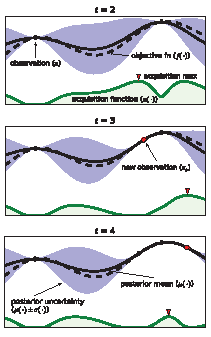
\includegraphics[width=0.99\textwidth]{figures/bayesian_optimization/bo.pdf}
  \caption[Bayesian Optimization]{XXX \TODO. Adapted from \citet{brochuTutorialBayesianOptimization2010}.}
  \label{fig:ml:bayesian_optimization}
\end{marginfigure}

Bayesian Optimization is better explained by looking at Figure~\ref{fig:ml:bayesian_optimization}. First look at the top plot. This is a plot of the surrogate function in black with uncertainties shown in blue. This is a result of fitting GPs to the two previous points in black, $t=2$. This surrogate function is supposed to fit the evaluation function (called objective in the figure) shown as a dashed black line. Below we see the acquisition function in green. This is a function of the blue curve and the position of its maximum decides where the next guess of $\bm{\lambda}$ should be. With the chosen acquisition function and exploration willingness, we see that the next guess should be slightly to the left of the right-most point. This is a simple 1D toy problem, but one should imagine this happening in a high-dimensional space. After making a new guess, $t=3$ in the middle plot, the acquisition function changes since it learnt that this gave a worse evaluation value than the right-most point. Therefore, the next proposal for $\bm{\lambda}$ is slighty to the right of the right-most point. The process continues like this in an iterative fashion: first fitting GPs to the previous evaluation values and then choosing the next $\bm{\lambda}$ according the acquisition function given the GPs. 

Gaussian Processes provide a posterior distribution given some prior distribution and the datadependent ikelihood. The process of BO is quite technical and mathematical, especially if GPs are new material. For a more in-depth explanation of the topic, see \citet{brochuTutorialBayesianOptimization2010}. The important thing to note is that GPs return not only a posterior mean $\mu(\vec{x})$ but also an uncertainty $\sigma(\vec{x})$, as seen in Figure~\ref{fig:ml:bayesian_optimization} described above. The acquisition function used in this project is the Upper Confidence Bound (UCB):
\begin{equation}
  \mathrm{UCB}(\vec{x}) = \mu(\vec{x}) + \kappa \sigma(\vec{x}),
\end{equation}
where $\kappa \geq 0$ is the parameter\sidenote{Here $\kappa$ can thus be regarded as a hyper-hyperparameter since it controlls how the other hyperparamaters are optimized.} controlling the exploration-exploitation tradeoff. 

Bayesian Optimization has the great benefit of slowly learning the hyperparameter space and making smarter and more educated guesses over time. However, it also comes with the cost of being harder to numerically implement compared to GS and RS\sidenote{Which are basically plug-and-play with Scikit-Learn \autocite{scikit-learn}.}, and parallelization is non-trivial to implement since it by definition is a sequential process. The performance boost is also not guaranteed. 

\section{Feature Importance}
\label{sec:ml:feature_importance}
Having first established in \autoref{sec:ml:supervised_learning} that machine learning algorithms are indeed able to not only learn from data but also to generalize well without overfitting (\autoref{sec:ml:overfitting}), modern ML algorithms such as decision trees, random forests and boosted decision trees were introduced in \autoref{sec:ml:decision_trees} and they were hyperparameter optimized in \autoref{sec:ml:hyperparameter_optimization}, one would expect that one would have a well performing model by now. 

Now comes one of the most important issues in ML today: model inspection. Actually trying to make sense of the learnt model. Why does it predict as it does? Which features or variables are most important according to the model? Model interpretation is still very much active research today with no universally accepted methods. Some methods are model dependent and accurate, others might be model agnostic but slow or only approximations. In this project the focus will be on the so-called \emph{SHAP} values. 

In 2017 \citet{Lundberg:2017} showed that six different previously used methods were all specific instances of a universal underlying method\sidenote{The class of \emph{additive feature attribution methods} \citep{Lundberg:2017}.} and propose SHaplay Additive exPlanation (SHAP) values as a unified measure of feature importance. In 2018-2019 they developed a fast algorithm for computing SHAP values for tree ensemples and showed that previous measures of feature importance heavily used for trees, e.g. \emph{gain}, were \emph{inconsistent} \autocite{lundbergConsistentIndividualizedFeature2019}. That a measure for feature importance is inconsistent means that a model could rely more on feature $A$ than $B$, however, the feature importance would indicate opposite. SHAP values and \emph{permutation} feature importance are both consistent feature importance measure, however, only SHAP allows for individualized\sidenote{Meaning that you can get the feature importances for a single observation compared to only the global, overall feature importances as seen across the entire data set.}, or local, feature importances.  

SHAP values are within the class of additive feature attribution methods, which are functions where the explanation model $g$ is a linear combination of binary variables:
\begin{equation}
  \label{eq:ml:additive_feature_attribution_method}
  g(z') = \phi_0 + \sum_{i=1}^M \phi_i z_i'.
\end{equation}
Here $\phi_i \in \mathbb{R}$ are the feature importances and $z'$ is a binary variable such that $z_i'=1$ if the feature is present and otherwise $z_i' = 0$. SHAP values are based on Shapley regression values known from cooperative game theory \autocite{Shapley1953}. These values are based on the three axioms:
\begin{axiom}[Local Accuracy]
  Local accuracy says that the sum of the feature importances should equal the total reward:
  \begin{equation}
    f(x) = g(z') = \phi_0 + \sum_{i=1}^M \phi_i z_i'.
  \end{equation}
\end{axiom}
Here $f$ is the ML model, $g$ is the explanation model, $x$ is an observation in input feature space, $z'$ is an observation in the binary space as described above, and $\phi_i$ is the feature importance. 
\begin{axiom}[Missingness]
  Missingness means that features missing in the original input feature space (such that $z_i'=0$) should be attributed no importance:
  \begin{equation}
    z_i' = 0 \Rightarrow \phi_i = 0.
  \end{equation} 
\end{axiom}
\begin{axiom}[Consistency]
  \label{axiom:ml:shap_consistency}
  Consistency states if a model is changed such that it relies more on a certain feature, the feature importance of that feature should never decrease. 
\end{axiom}
% \begin{description}
%   \item[Local Accuracy] 
%   Local accuracy says that the sum of the feature importances should equal the total reward:
%   \begin{equation}
%     f(x) = g(x') = \phi_0 + \sum_{i=1}^N \phi_i x_i'.
%   \end{equation}
%   Here $f$ is the ML model, $g$ is the explanation model, $x$ is an observation in input feature space, $x'$ is an observation in the binary space as described above, and $\phi_i$ is the feature importance. 

%   \item[Missingness] Missingness means that features missing in the original input feature space (such that $x_i'=0$) should be attributed no importance:
%   \begin{equation}
%     x_i = 0 \Rightarrow \phi_i = 0
%   \end{equation}
%   \item[Consistency] Consistency states if a model is changed such that it relies more on a certain feature, the feature importance of that feature should never decrease.
% \end{description}
Given these three axioms, \citet{Lundberg:2017} show that the only solution to equation \eqref{eq:ml:additive_feature_attribution_method} is:
\begin{equation}
  \label{eq:ml:shap_feature_importance}
    \phi_i = \sum_{S \subseteq \widetilde{M} \backslash \{i\}} \frac{|S|!(M-|S|-1)!}{M!} \left[ f_x(S \cup \{i\}) - f_x(S) \right] ,
\end{equation}
which one can simplify to:
\begin{equation}
  \label{eq:ml:shap_feature_importance_simplification}
  \begin{split}
    \phi_i        &= \sum_{S \subseteq \widetilde{M} \backslash \{i\}} w(S) \cdot \Delta_{f_x}(S) \\
    w(S)             &\equiv \frac{|S|!(M-|S|-1)!}{M!} \\
    \Delta_{f_x}(S)  &\equiv \left[ f_x(S \cup \{i\}) - f_x(S) \right].
  \end{split}
\end{equation}


In equation \eqref{eq:ml:shap_feature_importance} $\widetilde{M}$ is the \emph{set} of all input features\sidenote{Compared to $M=|\widetilde{M}|$ which is the \emph{number} of all input features.}, $S \subseteq \widetilde{M} \backslash \{i\}$ means a subset $S$ of $\widetilde{M}$ without feature $i$, $S \cup \{i\}$ means the set $S$ with feature $i$ and $f_x(S) = f(h_x(z'))$ where $h_x(z')$ is the mapping function from the binary $z'$ space to the input feature space $x$. In equation \eqref{eq:ml:shap_feature_importance_simplification} the function is simplified to its basic constituents: the difference in performance  between including feature $i$ and not including it, $\Delta_{f_x}$, and its weight $w$. 

To get a better understanding of the different sets in the summation, one could look at the decision tree shown in Figure~\ref{fig:ml:decision_tree}. Here $\widetilde{M}$ would be $\widetilde{M}=\{p_\perp, E_\mathrm{jet} \}$. For the feature $i=p_\perp $ one would thus have:
\begin{equation}
  \begin{split}
    \phi_{p_\vert} = & \sum_{S \subseteq \widetilde{M} \backslash \{p_\perp \}} w(S)  \cdot\Delta_{f_x}(S)  \\
                   = & \sum_{S \in \left[\{\}, \{E_\mathrm{jet}\} \right]} w(S)  \cdot\Delta_{f_x}(S)  \\
                   = & \frac{0! (2-0-1)!}{2!}  [ f_x(\{p_\perp\}) - f_x(\{\})]  \\ 
                     & +    \frac{1! (2-1-1)!}{2!}  [f_x(\{ E_\mathrm{jet}, p_\perp \}) - f_x(\{ E_\mathrm{jet} \})].
  \end{split}
\end{equation}
Whereas $w(S)$ are easily calculated, $\Delta_{f_x}$ depends on the data. As the number of features grows, the number of terms in the sum grows exponentially. What \citet{lundbergConsistentIndividualizedFeature2019} did was to develop an efficient algorithm that could solve this for trees in polynomial time\sidenote{Specifically they managed to improve the time complexity from $\mathcal{O}(TL2^M)$ to $\mathcal{O}(TLD^2)$ where $T$ is the number of trees, $L$ is the maximum number of leaves in any tree, $M$ is te number of features, and $D$ is the maximum depth of any tree (where $D\approx \log L$ for balanced trees).}. 

SHAP values allows one to explain for a single prediction why it got the prediction that it got. When applied to the entire data set $\vec{X} \in \mathbb{R}^{N \times M}$ with $N$ observations each of with $M$ features, one gets the matrix $\bm{\Phi}$. When summing over the absolute value of each column, one gets the global impact $\phi_i^\mathrm{tot}$ of the $i^{\mathrm{th}}$ feature \citep{lundbergConsistentIndividualizedFeature2019}:
\begin{equation}
  \phi_i^\mathrm{tot} = \sum_{j=1}^N \abs{ \bm{\Phi}_{i, j} }.
\end{equation}
The global feature importance $\phi_i^\mathrm{tot}$ is thus a measure of the overall importance of feature $i$. 

Note that if one introduces a new feature to the dataset, correlated\sidenote{Not necessarily linearly correlated.} to an already existing feature, the feature importance of the previous feature will decrease. 
This is due to the axiom of symmetry:
\begin{axiom}[Symmetry]
  \label{axiom:ml:shapley_symmetry}
  If for all subsets S that do not contain $i$ or $j$: 
  \begin{equation}
    f_x(S \cup \{i\}) = f_x(S \cup \{j\})
  \end{equation}
  then $\phi_i = \phi_j$.
\end{axiom}
It can be shown that axiom \ref{axiom:ml:shapley_symmetry} is implied by axiom \ref{axiom:ml:shap_consistency}  \citep[Supp. Material]{Lundberg:2017}. Two identical features, as seen by the model, will thus \q{share} the feature importance.


\chapter{Housing Prices Analysis}
\label{ch:housing_price_analysis}

\begin{figure}
  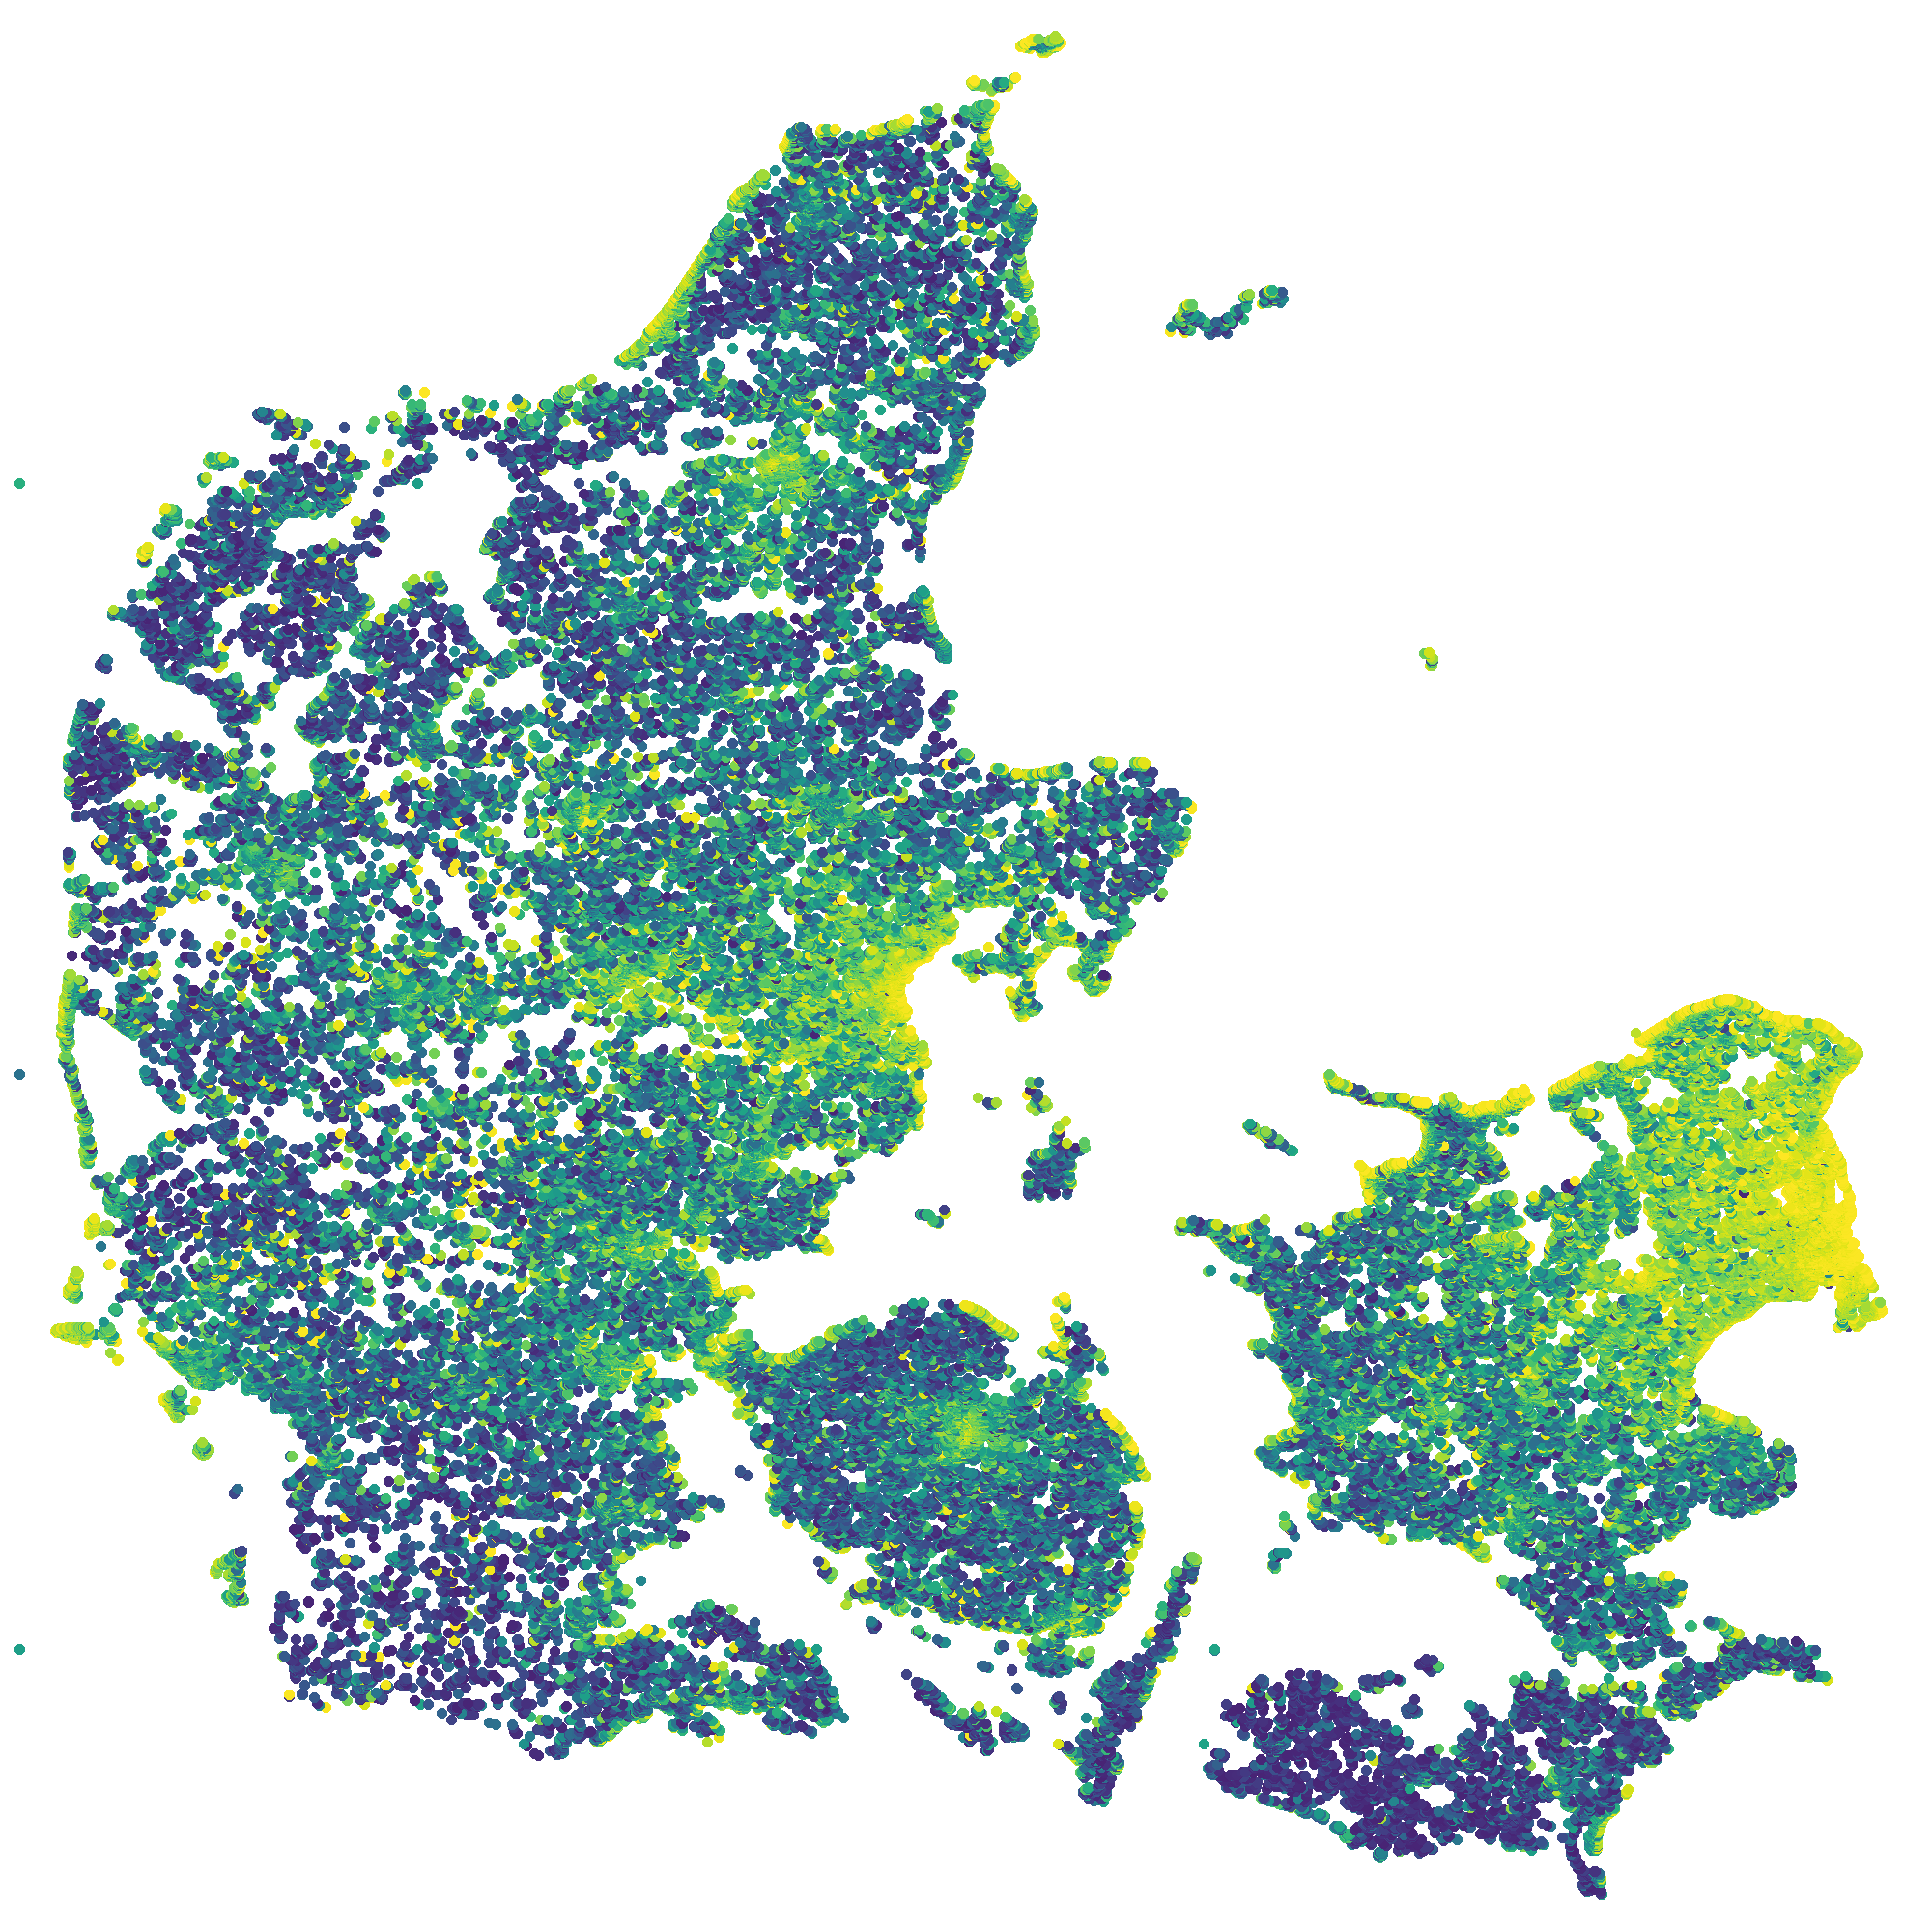
\includegraphics[width=0.9\textwidth, trim=0 0 0 0, clip]{figures/housing/Denmark_Overview_SqmPrice.png}
  \caption[Geographic overview of square meter price in Denmark][6pt]
          {Geographic overview of square meter prices for houses and apartments in Denmark (excluding Bornholm for visual purposes). Notice the strong correlation with the major cities and the shore line. Also notice the three outliers west of Jutland. }
  \label{fig:h:geo_overview}
\end{figure}



\begin{figure}
  \includegraphics[width=0.9\textwidth, page=2]{figures/housing/overview_fig.pdf}
  \caption[Histogram of prices of houses and apartments sold in Denmark][6pt]
          {Histogram of prices of houses and apartments sold in Denmark.}
  \label{fig:h:price_overview}
\end{figure}


\begin{figure*}[htb]
  \centering
  
  \vspace*{-\abovecaptionskip}
  
  \subfloat[\label{fig:h:variable_overview_a}]{\qquad}
  \includegraphics[width=0.4\textwidth, page=2]{figures/housing/overview_fig.pdf}\hfil
  \subfloat[\label{fig:h:variable_overview_b}]{\qquad}
  \includegraphics[width=0.4\textwidth, page=6]{figures/housing/overview_fig.pdf}

  \subfloat[\label{fig:h:variable_overview_c}]{\qquad}
  \includegraphics[width=0.4\textwidth, page=20]{figures/housing/overview_fig.pdf}\hfil
  \subfloat[\label{fig:h:variable_overview_d}]{\qquad}
  \includegraphics[width=0.4\textwidth, page=23]{figures/housing/overview_fig.pdf}
  
  \caption[Input paramater distributions for the housing prices dataset]{Distributions of the four out of the XXX input variables. Subplot ~\protect\subref{fig:h:variable_overview_a} shows the date of the sale, 
           Subplot ~\protect\subref{fig:h:variable_overview_b} shows the type of sale,
           Subplot ~\protect\subref{fig:h:variable_overview_c} shows the longitude,
           Subplot ~\protect\subref{fig:h:variable_overview_d} shows the area,}
  \label{fig:h:variable_overview}
  
  \vspace{\abovecaptionskip}
\end{figure*}


Outside referencing isn't different: In fig.~\ref{fig:h:variable_overview}: Two images --- fig.~\subref{fig:h:variable_overview_a} shows an "A", fig.~\subref{fig:h:variable_overview_b} shows a "B".



\begin{figure}
  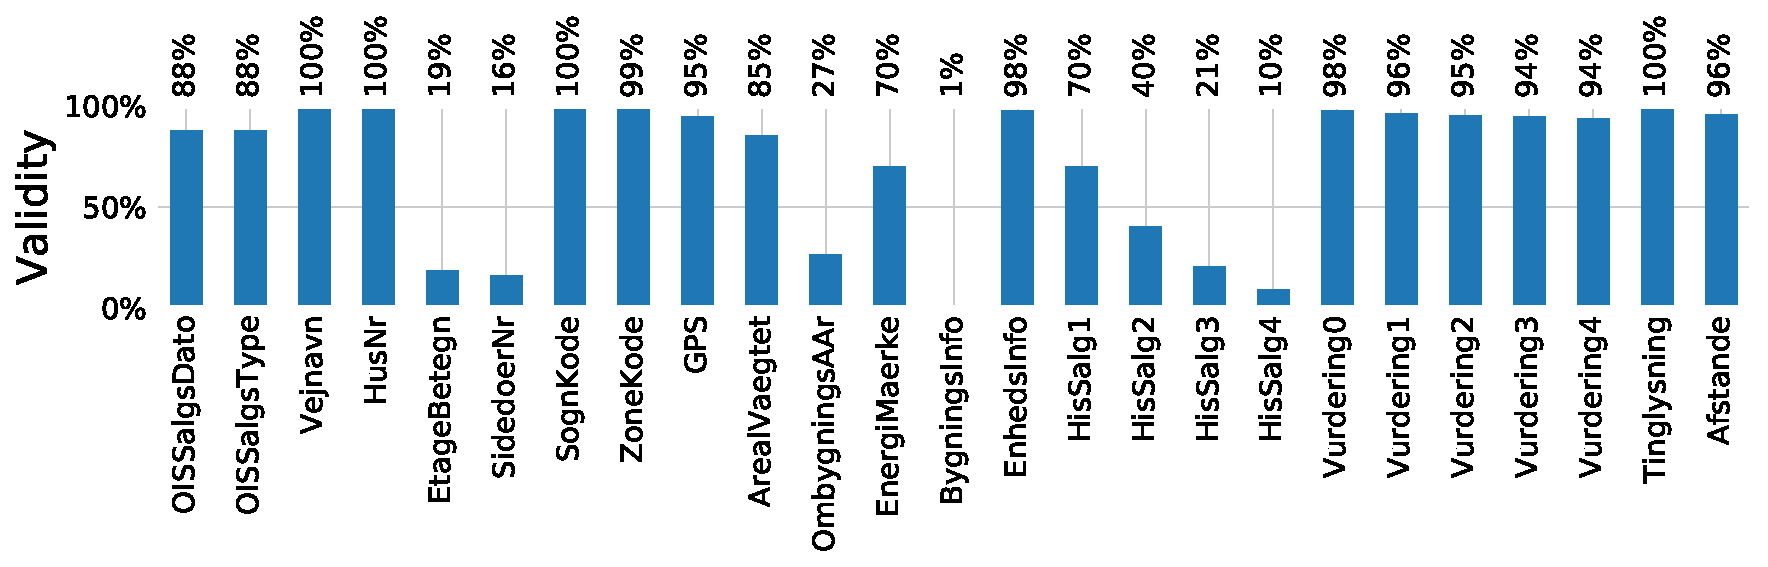
\includegraphics[width=0.9\textwidth, trim=0 0 0 40, clip]{figures/housing/missing_bar.pdf}
  \caption[Percentage of valid counts for each variable][6pt]
          {Percentage of valid counts for each variable grouped together in categories.}
  \label{fig:h:nans}
\end{figure}


\begin{figure}
  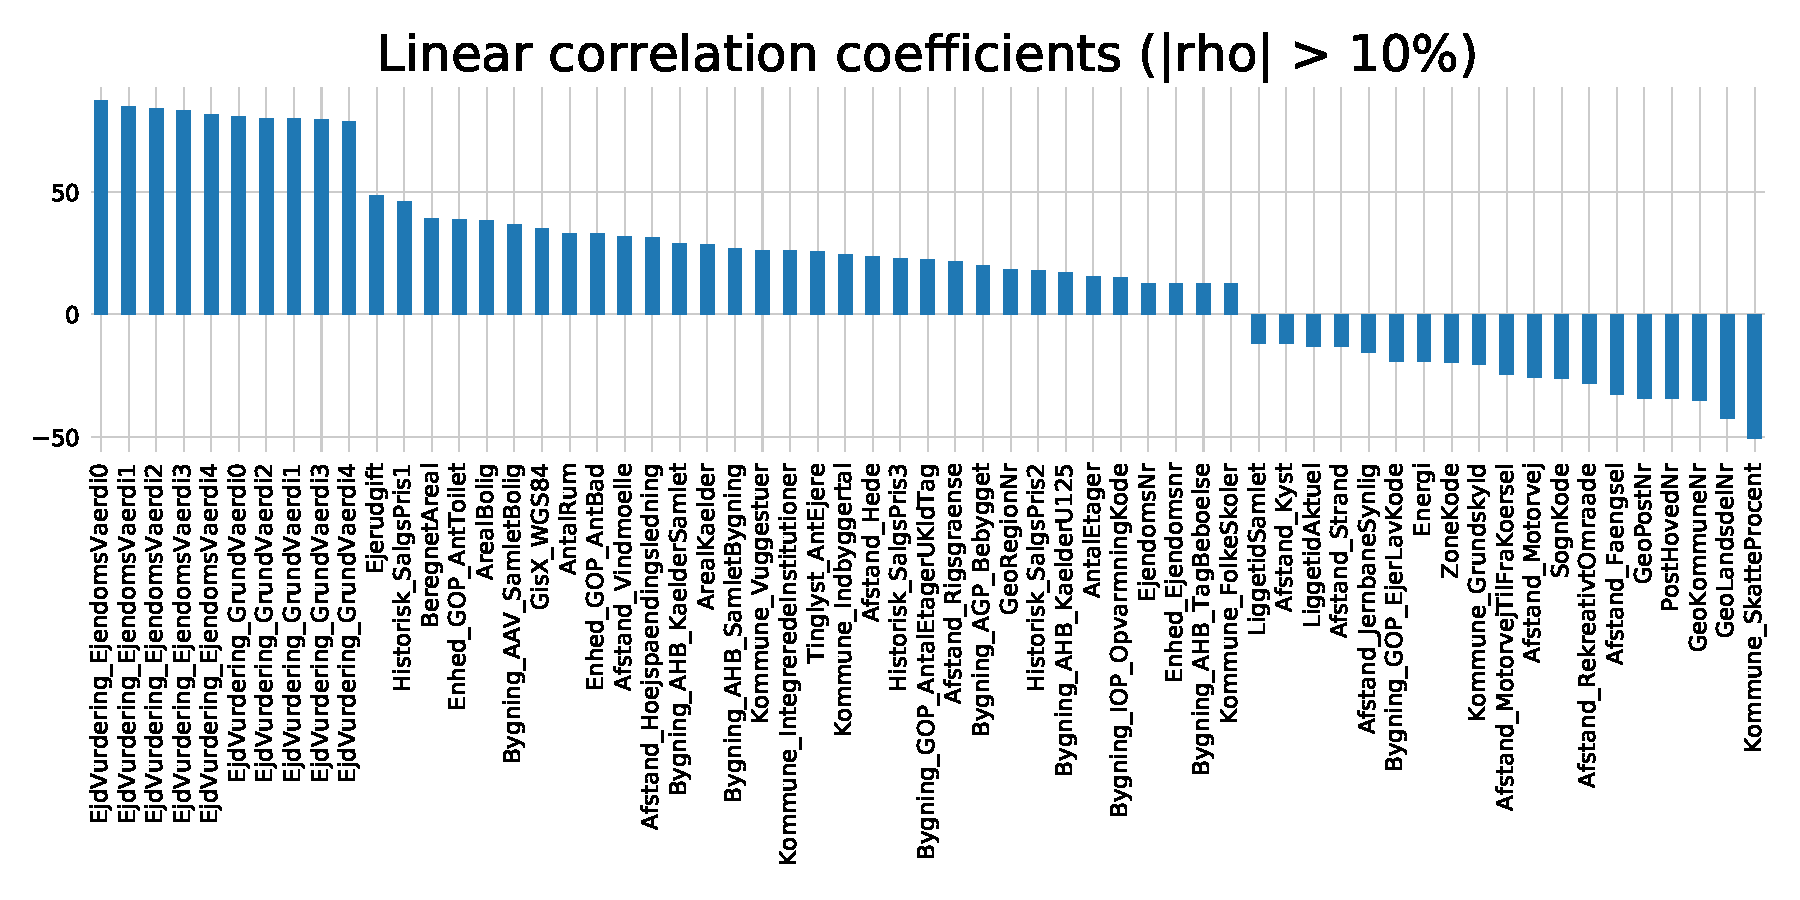
\includegraphics[width=0.9\textwidth, trim=0 0 0 40, clip]{figures/housing/lin_correlation.pdf}
  \caption[Linear correlation between variables and price][6pt]
          {Linear correlation between variables and price for variables where the correlation coefficient $\rho$ is $|\rho| > 10\%$.}
  \label{fig:h:corr_lin}
\end{figure}

\begin{figure}
  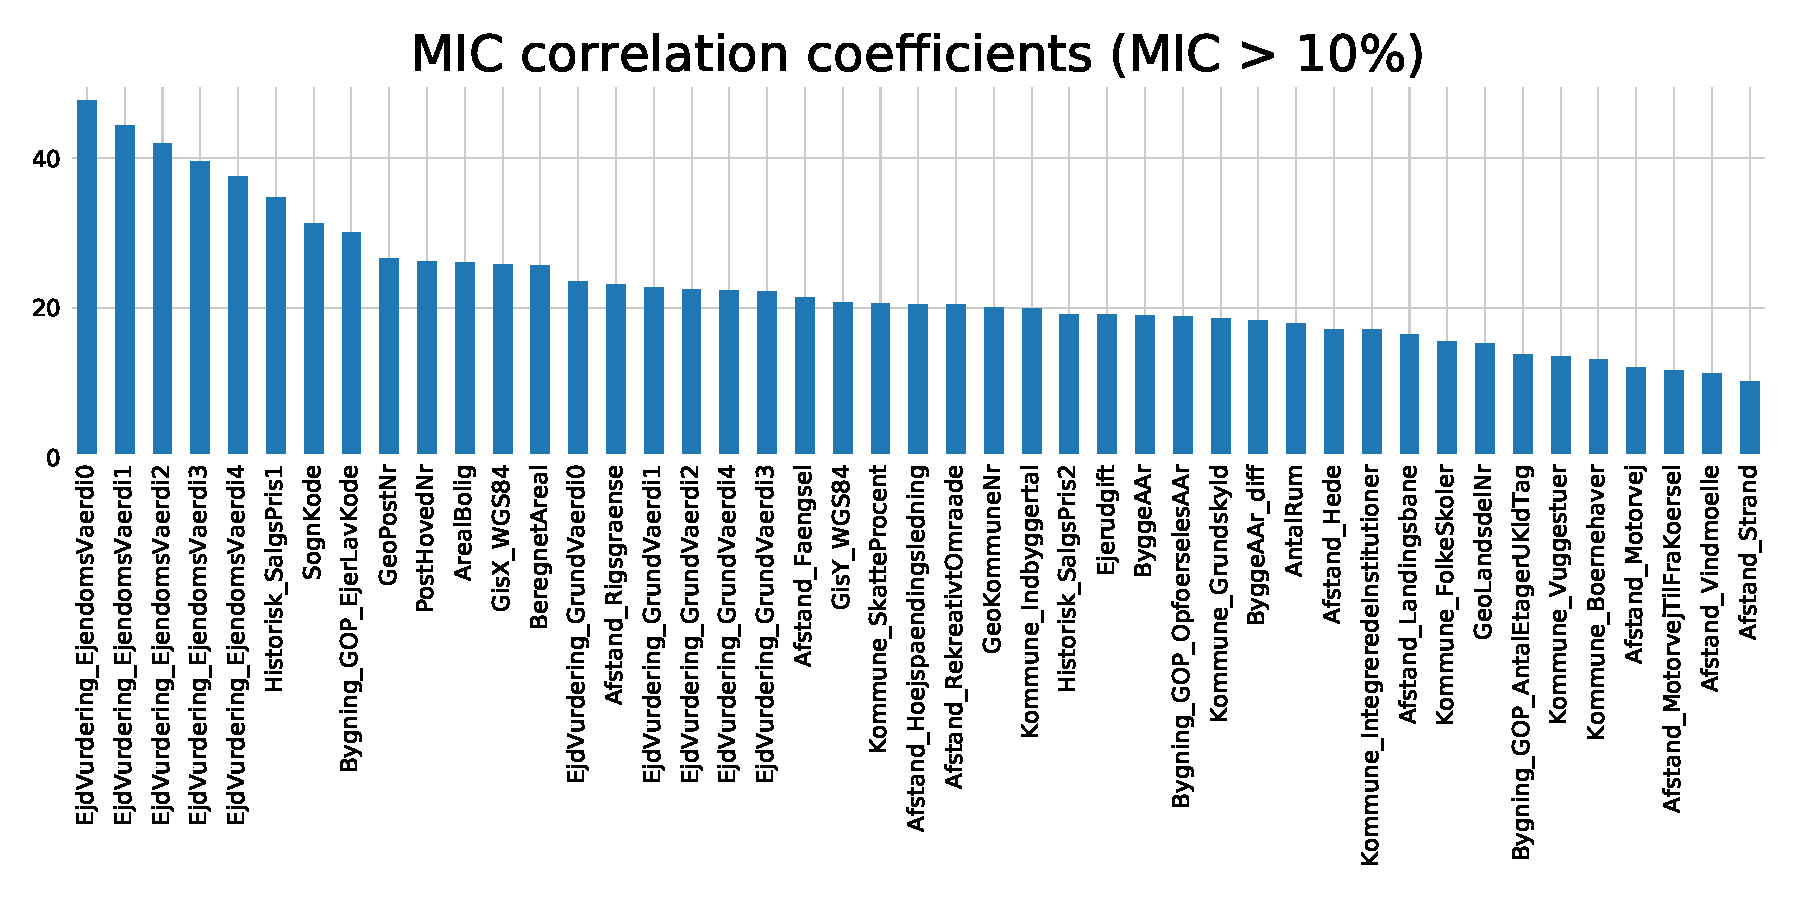
\includegraphics[width=0.9\textwidth, trim=0 0 0 40, clip]{figures/housing/MIC_plot.pdf}
  \caption[Non-linear correlation between variables and price][6pt]
          {Non-linear correlation between variables and price using Maximal Information Coefficient (MIC) for variables where $\text{MIC}>10\%$.}
  \label{fig:h:corr_MIC}
\end{figure}

\begin{figure}
  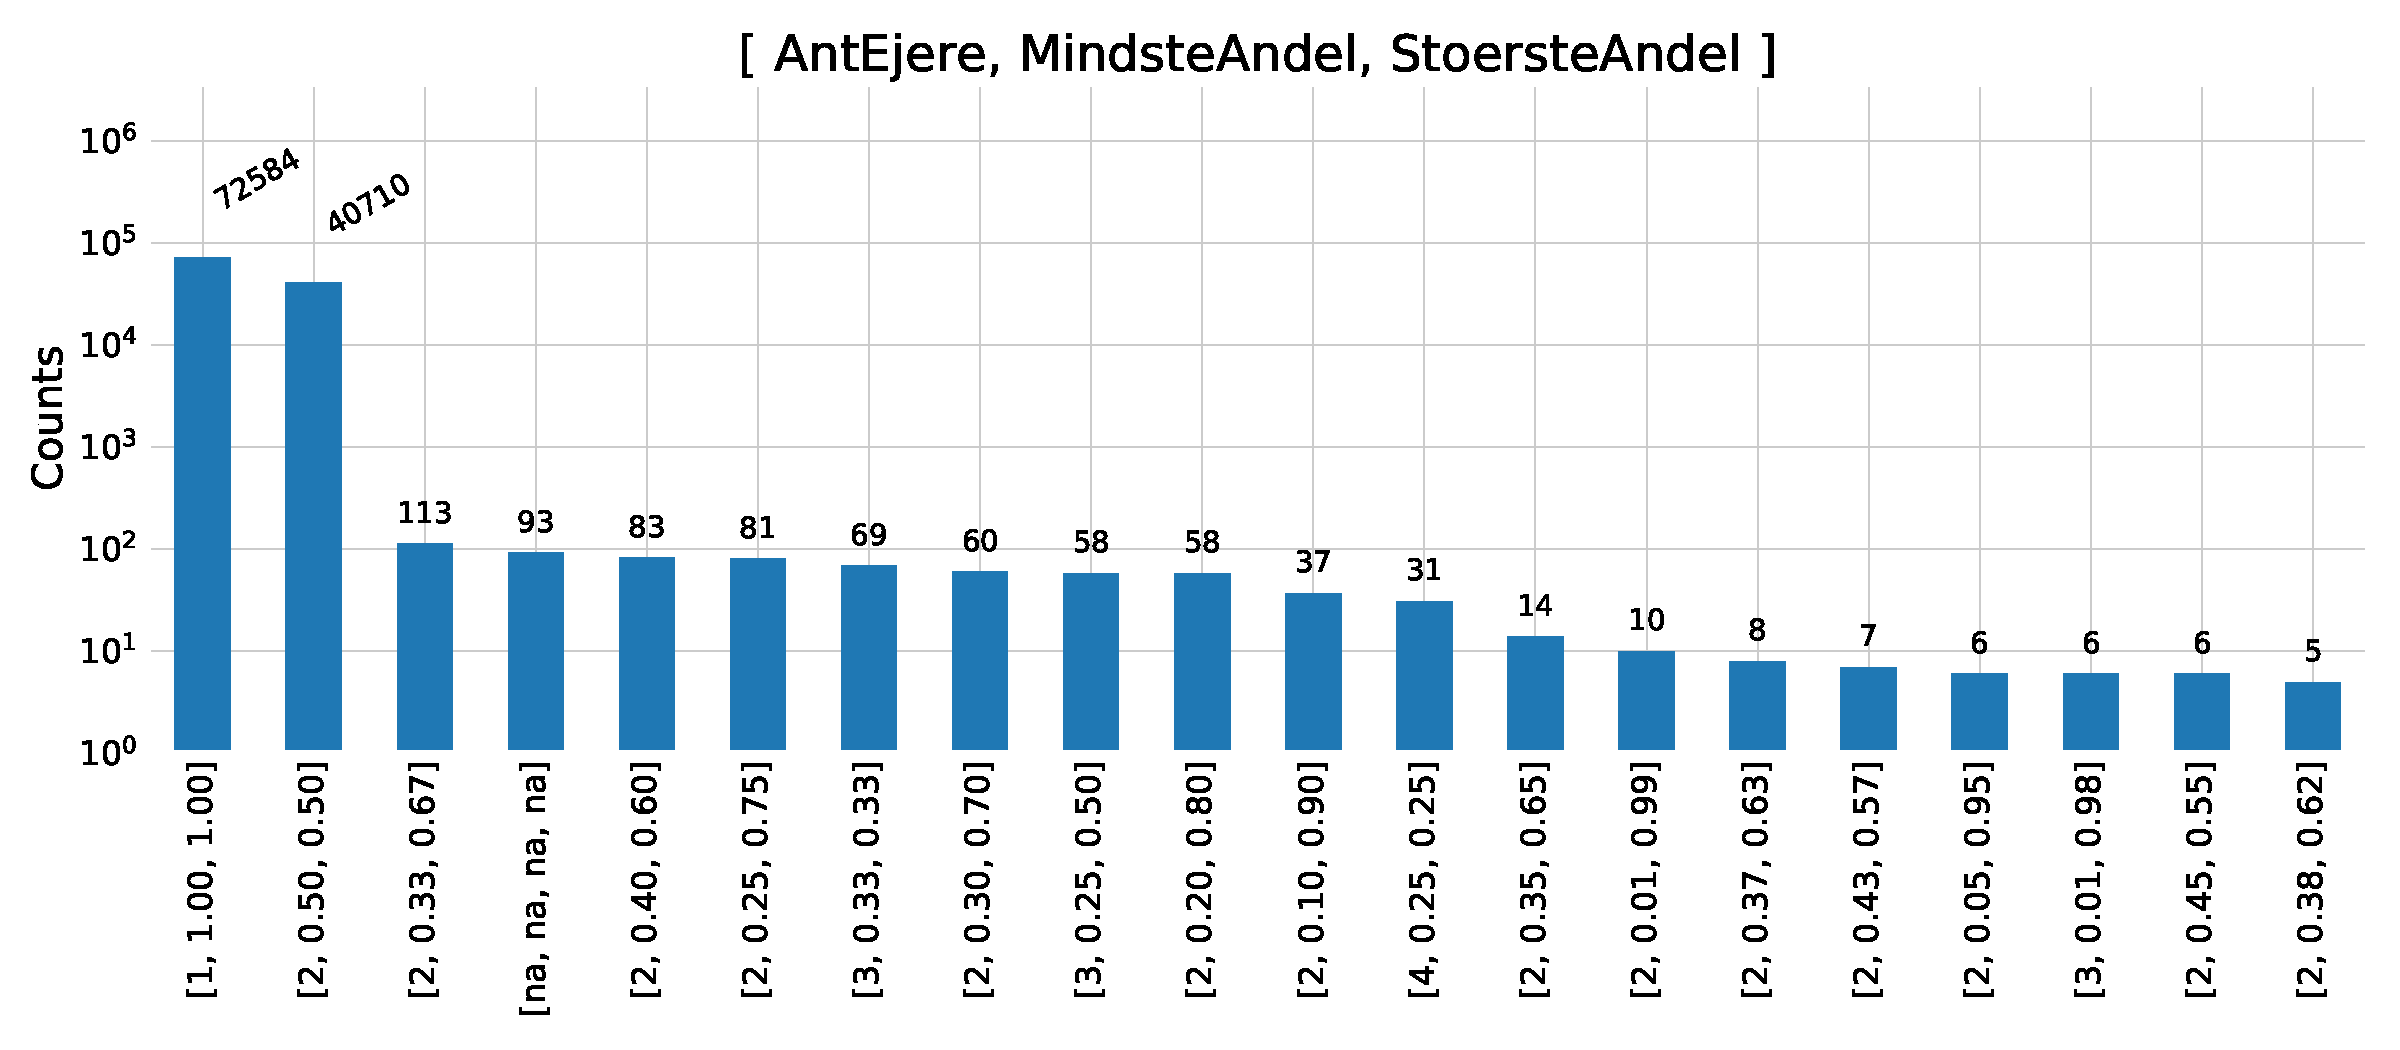
\includegraphics[width=0.9\textwidth]{figures/housing/tinglysning_fig.pdf}
  \caption[Registration of property][6pt]
          {Overview of registration of property as a function of amount of owners (\code{AntEjere}), lowest share (\code{MindsteAndel}) and biggest share (\code{StoersteAndel}) written as \code{[AntEjere, MindsteAndel, StoersteAndel]}.
          }
  \label{fig:h:tinglysning}
\end{figure}



\begin{figure}
  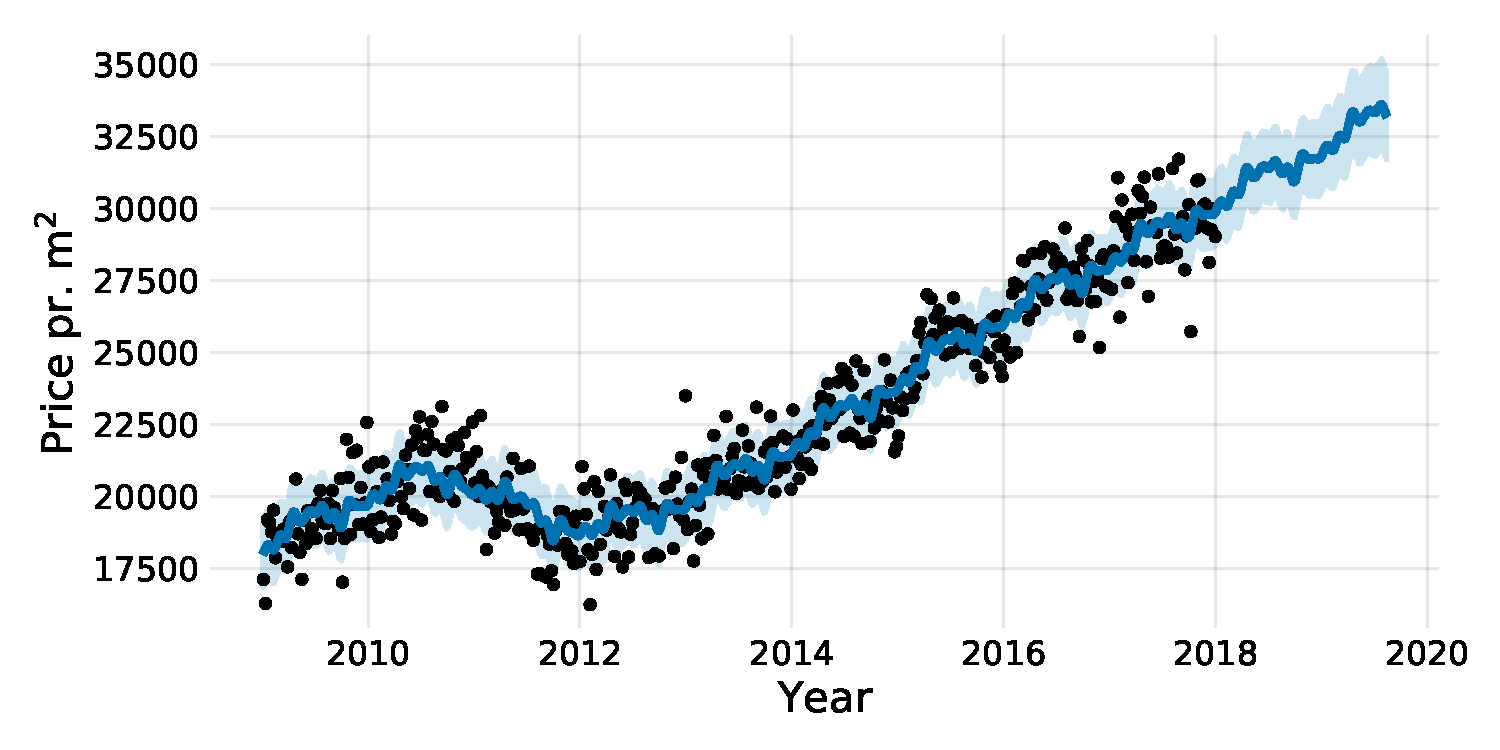
\includegraphics[width=0.9\textwidth]{figures/housing/Ejerlejlighed_v17_cut_all_Ncols_all_prophet_forecast.pdf}
  \caption[Prophet Forecast for apartments][6pt]
          {The predictions of the Facebook Prophet model trained on square meter prices for apartments sold before January 1st, 2018. The data is down-sampled to weekly bins where the median of each week is used as in input to the Prophet model. This can be seen as black dots in the figure. The \textcolor{blue}{model's forecasts} for 2018 and 2019 are shown in blue with a light blue \textcolor{light-blue}{error band} showing the 1-sigma confidence interval.
          }
  \label{fig:h:prophet_forecast}
\end{figure}


\begin{figure}
  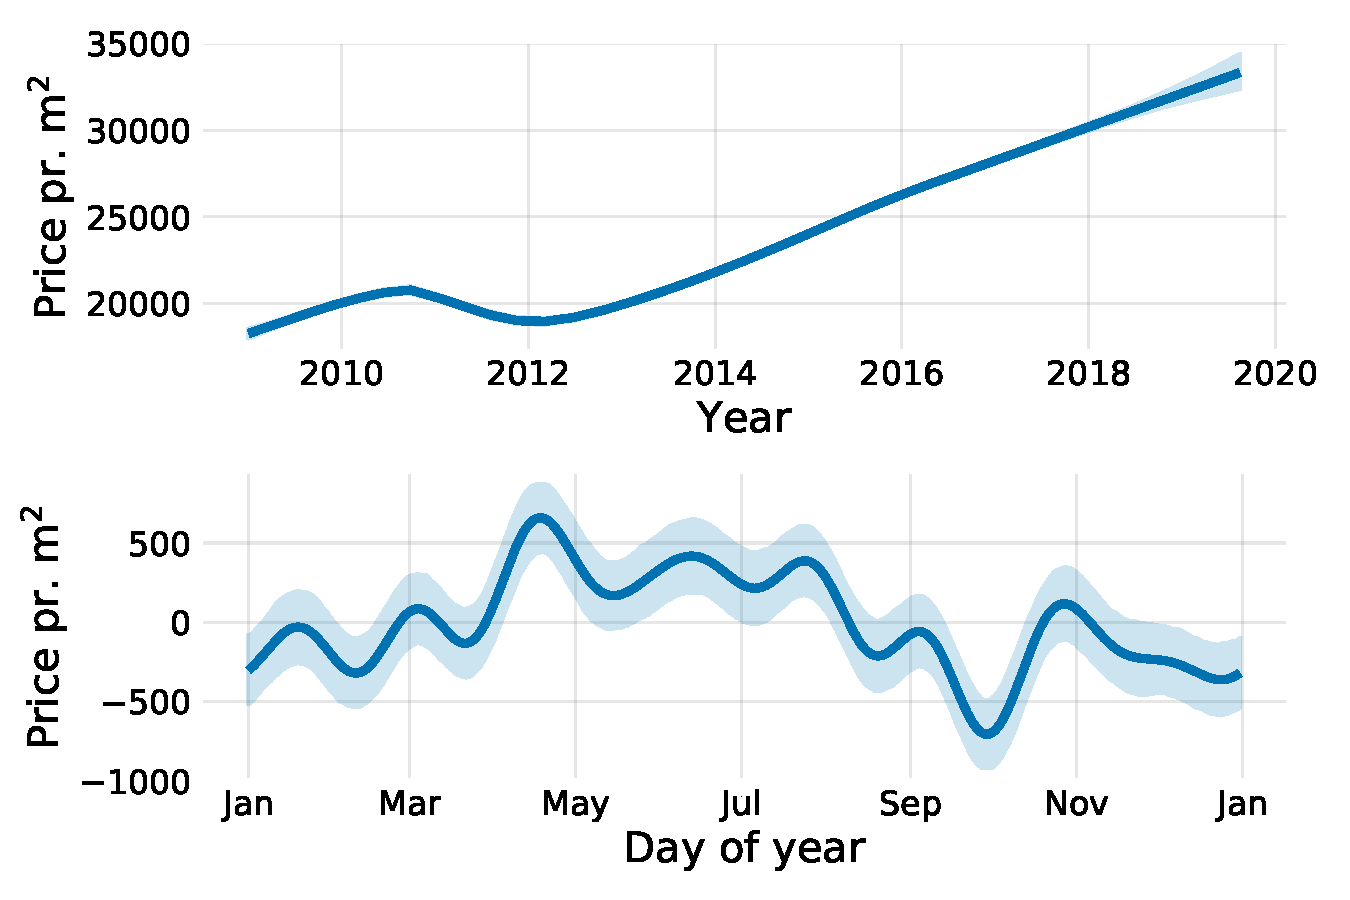
\includegraphics[width=0.9\textwidth]{figures/housing/Ejerlejlighed_v17_cut_all_Ncols_all_prophet_trends.pdf}
  \caption[Prophet Trends][6pt]
          {The trends of the Facebook Prophet model trained on square meter prices for apartments sold before January 1st, 2018. In the top plot is the overall trend as a function of year and in the bottom plot is the yearly variation as a function of day of year. It can be seen that the square meter price is higher during the Summer months compared to the Winter months, however, compared to the overall trend this effect is minor ($<10\%$). 
          }
  \label{fig:h:prophet_trends}
\end{figure}



% \begin{table}[]
  % \begin{tabular}{@{}lllll@{}}

\begin{table}[]
  \begin{tabular}{@{}llrrl@{}}
    \toprule
  Halflife & $\log_{10}$ & $N_\mathrm{trees}$ & Time [$s$]   & MAD    \\ \midrule
  2.5 & True & 210 & 81  & 0.1651 \\
  2.5 & False & 217 & 64  & 0.1791 \\
  5   & True & 209 & 78  & 0.1647 \\
  5   & False & 100 & 41  & 0.1950  \\
  \textbf{10}  & \textbf{True} & \textbf{375} & \textbf{118} & \textbf{0.1563} \\
  10  & False & 411 & 97   & 0.1739 \\
  20  & True & 333 & 106 & 0.1639 \\
  20  & False & 125 & 44  & 0.1925 \\
  $\infty$   & True & 371 & 112 & 0.1596 \\
  $\infty$   & False & 79  & 30  & 0.2062 \\ \bottomrule
  \end{tabular}
  \caption{\label{tab:h:HPO_initial_RMSE}RMSE.}
  \end{table}
  
  \begin{table}[]
  \begin{tabular}{@{}llrrl@{}}
    \toprule
  Halflife & $\log_{10}$ & $N_\mathrm{trees}$ & Time [$s$]   & MAD    \\ \midrule
  2.5 & True & 180 & 57  & 0.1650  \\
  \textbf{2.5} & \textbf{False} & \textbf{682} & \textbf{111} & \textbf{0.1500}   \\
  5   & True & 198 & 62  & 0.1647 \\
  5   & False & 892 & 139 & 0.1514 \\
  10  & True & 244 & 68  & 0.1627 \\
  10  & False & 381 & 65  & 0.1608 \\
  20  & True & 396 & 95  & 0.1612 \\
  20  & False & 302 & 53   & 0.1626 \\
  $\infty$   & True & 239 & 60  & 0.1639 \\
  $\infty$   & False & 303 & 50   & 0.1620  \\ \bottomrule
  \end{tabular}
  \caption{\label{tab:h:HPO_initial_LogCosh}LogCosh.}
  \end{table}
  
  % \begin{table}[]
  % \begin{tabular}{@{}llrrl@{}}
  %   \toprule
  % Halflife & $\log_{10}$ & $N_\mathrm{trees}$ & Time [$s$]   & MAD    \\ \midrule
  % 2.5 & True & 267  & 75  & 0.1866 \\
  % 2.5 & False & 712  & 113 & 0.2794 \\
  % \textbf{5}   & \textbf{True} & \textbf{386}  & \textbf{91}  & \textbf{0.1843} \\
  % 5   & False & 394  & 60   & 0.2995 \\
  % 10  & True & 88   & 39  & 0.2426 \\
  % 10  & False & 215  & 39  & 0.3668 \\
  % 20  & True & 159  & 51  & 0.2152 \\
  % 20  & False & 604  & 89  & 0.3340  \\
  % $\infty$   & True & 326  & 82  & 0.1982 \\
  % $\infty$   & False & 1146 & 161 & 0.2963 \\ \bottomrule
  % \end{tabular}
  % \caption{\label{tab:h:HPO_initial_Cauchy}Cauchy.}
  % \end{table}
  
  % \begin{table}[]
  % \begin{tabular}{@{}llrrl@{}}
  %   \toprule
  % Halflife & $\log_{10}$ & $N_\mathrm{trees}$ & Time [$s$]   & MAD    \\ \midrule
  % 2.5    & True & 227  & 69  & 0.1973 \\
  % 2.5 & False & 621  & 99  & 0.4257 \\
  % 5   & True & 205  & 61  & 0.2128 \\
  % 5   & False & 320  & 53  & 0.4048 \\
  % \textbf{10}  & \textbf{True} & \textbf{286}  & \textbf{78}  & \textbf{0.1960}  \\
  % 10  & False & 1109 & 153 & 0.4045 \\
  % 20  & True & 171  & 53  & 0.2069 \\
  % 20  & False & 809  & 108  & 0.3698 \\
  % $\infty$   & True & 215  & 63  & 0.2194 \\
  % $\infty$   & False & 558  & 81  & 0.3933 \\ \bottomrule
  % \end{tabular}
  % \caption{\label{tab:h:HPO_initial_Welsch}Welsch.}
  % \end{table}
  
  % \begin{table}[]
  % \begin{tabular}{@{}llrrl@{}}
  %   \toprule
  % Halflife & $\log_{10}$ & $N_\mathrm{trees}$ & Time [$s$]   & MAD    \\ \midrule
  % 2.5 & True & 209 & 62 & 0.1631 \\
  % 2.5 & False & 170 & 37 & 0.1702 \\
  % 5   & True & 360 & 94 & 0.1623 \\
  % 5   & False & 252 & 49 & 0.1698 \\
  % \textbf{10}  & \textbf{True} & \textbf{368} & \textbf{93}  & \textbf{0.1574} \\
  % 10  & False & 322 & 53 & 0.1711 \\
  % 20  & True & 257 & 66 & 0.1614 \\
  % 20  & False & 313 & 50 & 0.1706 \\
  % $\infty$   & True & 351 & 85 & 0.1602 \\
  % $\infty$   & False & 360 & 57 & 0.1740  \\ \bottomrule
  % \end{tabular}
  % \caption{\label{tab:h:HPO_initial_Fair}Fair.}
  % \end{table}



\begin{figure}
  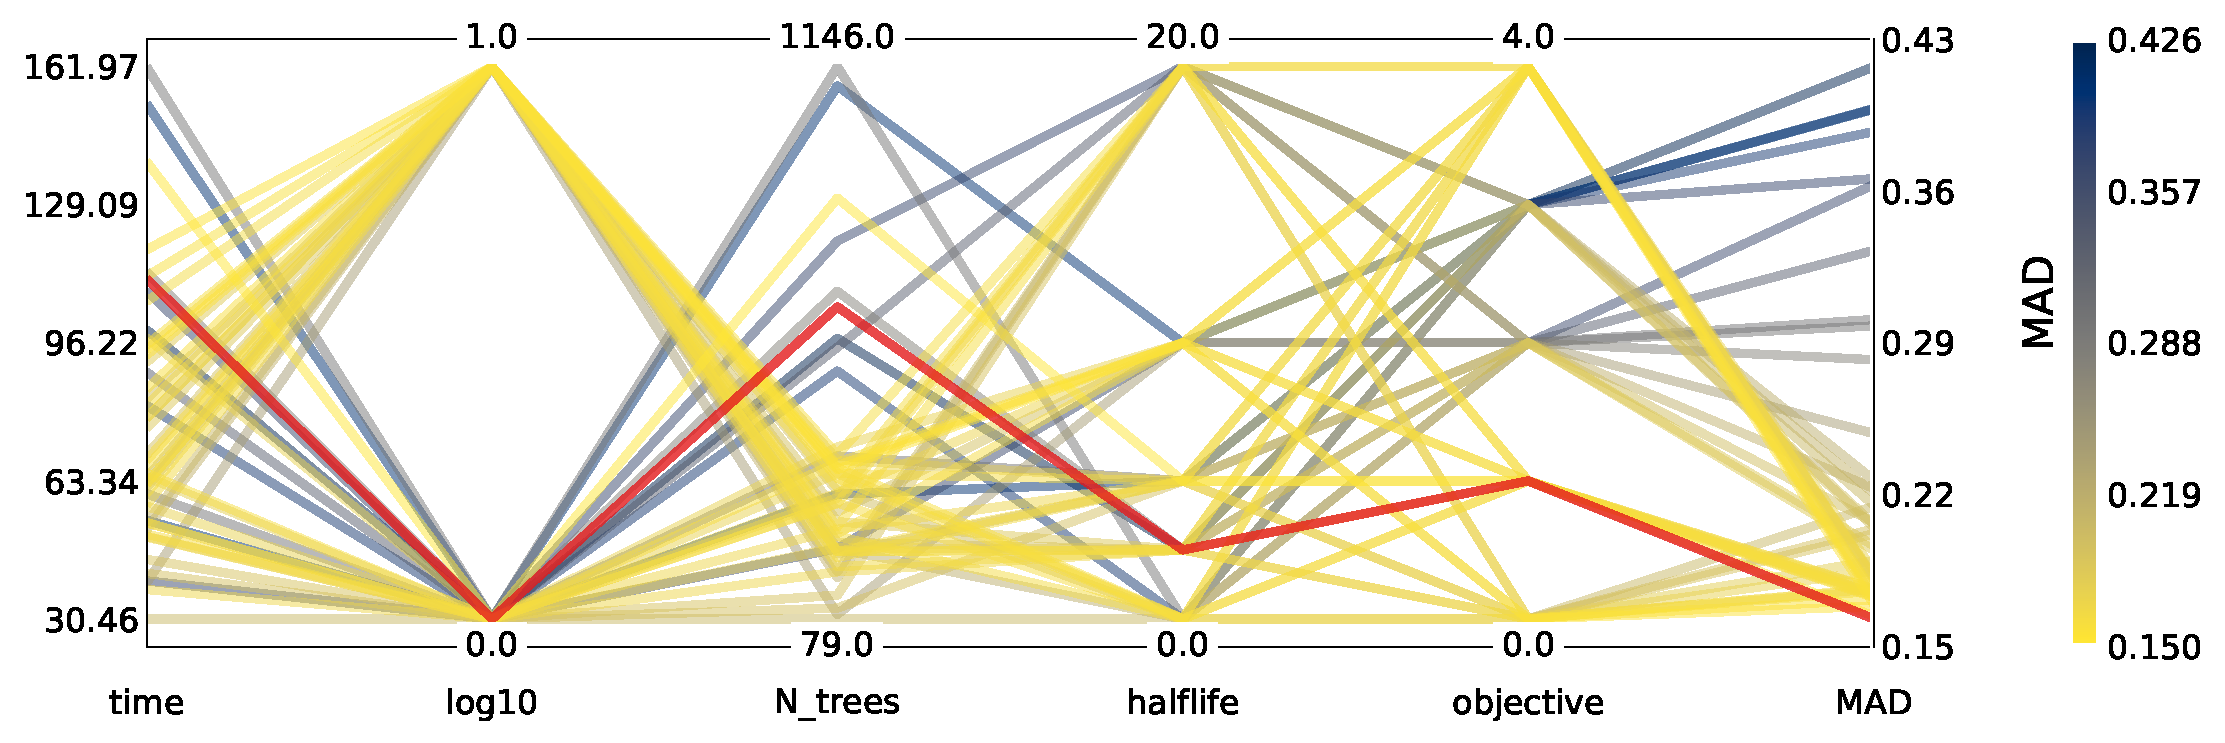
\includegraphics[width=0.95\textwidth, trim=0 0 0 0, clip]{figures/housing/Ejerlejlighed_v17_cut_all_Ncols_all_CV_viz_initial_HPO.pdf}
  \caption[Overview of initial hyperparamater optimization of the housing model for apartments][6pt]
          {Hyperparameter optimization results of the housing model for apartments. The results are shown as parallel coordinates with each hyperparameter along the x-axis and the value of that parameter on the y-axis. Each line is an event in the 4-dimensional space colored according to the performance of that hyperparameter as measured by MAD from \textcolor{viridis-dark}{highest} MAD in dark blue to \textcolor{viridis-light}{lowest} AUC in yellow. The \textcolor{red}{single best hyperparameter} is shown in red. For the hyperparamater \code{log10} \code{0} means False and \code{1} means True, for \code{objektive} the functions RMSE (0), LogCosh (1), Cauchy (2), Welsch (3), and Fair (4) are mapped to the integers in the parentheses.   
          } 
  \label{fig:h:CV_res_parallel_coords}
\end{figure}



\begin{figure}
  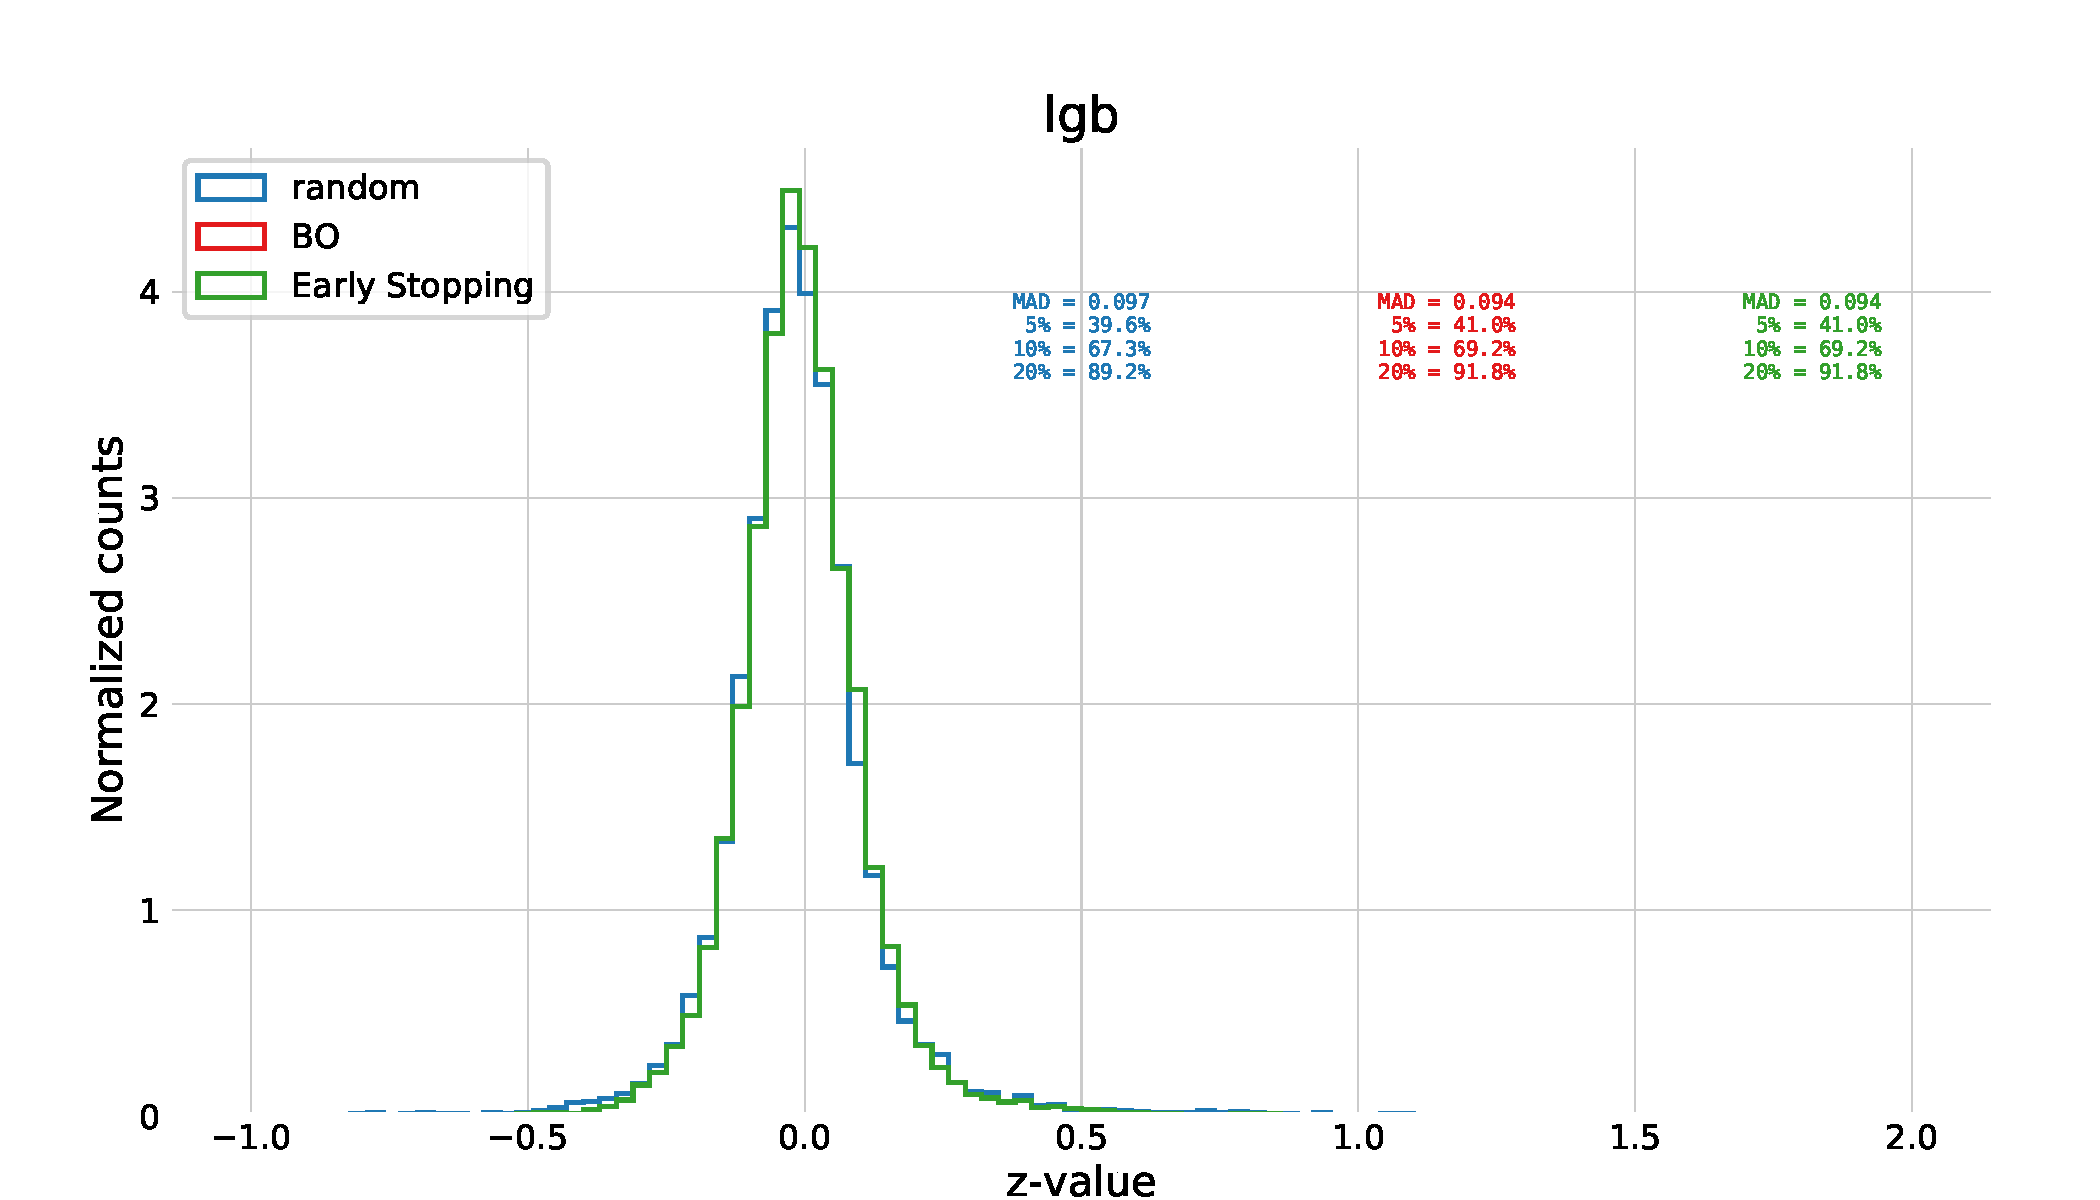
\includegraphics[width=0.9\textwidth, trim=0 0 0 70, clip]{figures/housing/Ejerlejlighed_v17_cut_all_Ncols_all_lgb_z_hist_metrics.pdf}
  \caption[Performance of LGB-model on apartment prices][6pt]
          {Histogram of $z$-values of the LGB-model trained on apartments. The performance after hyperparameter optimization (HPO) using \textcolor{blue}{Random Search} (RS) is shown in blue, for \textcolor{red}{Bayesian Optimization} (BO) in red. After finding the best model, BO in this case, the model is retrained using \textcolor{green}{early stopping}, the performance of which is shown in green.}
  \label{fig:h:performance_lgb}
\end{figure}


\begin{figure}
  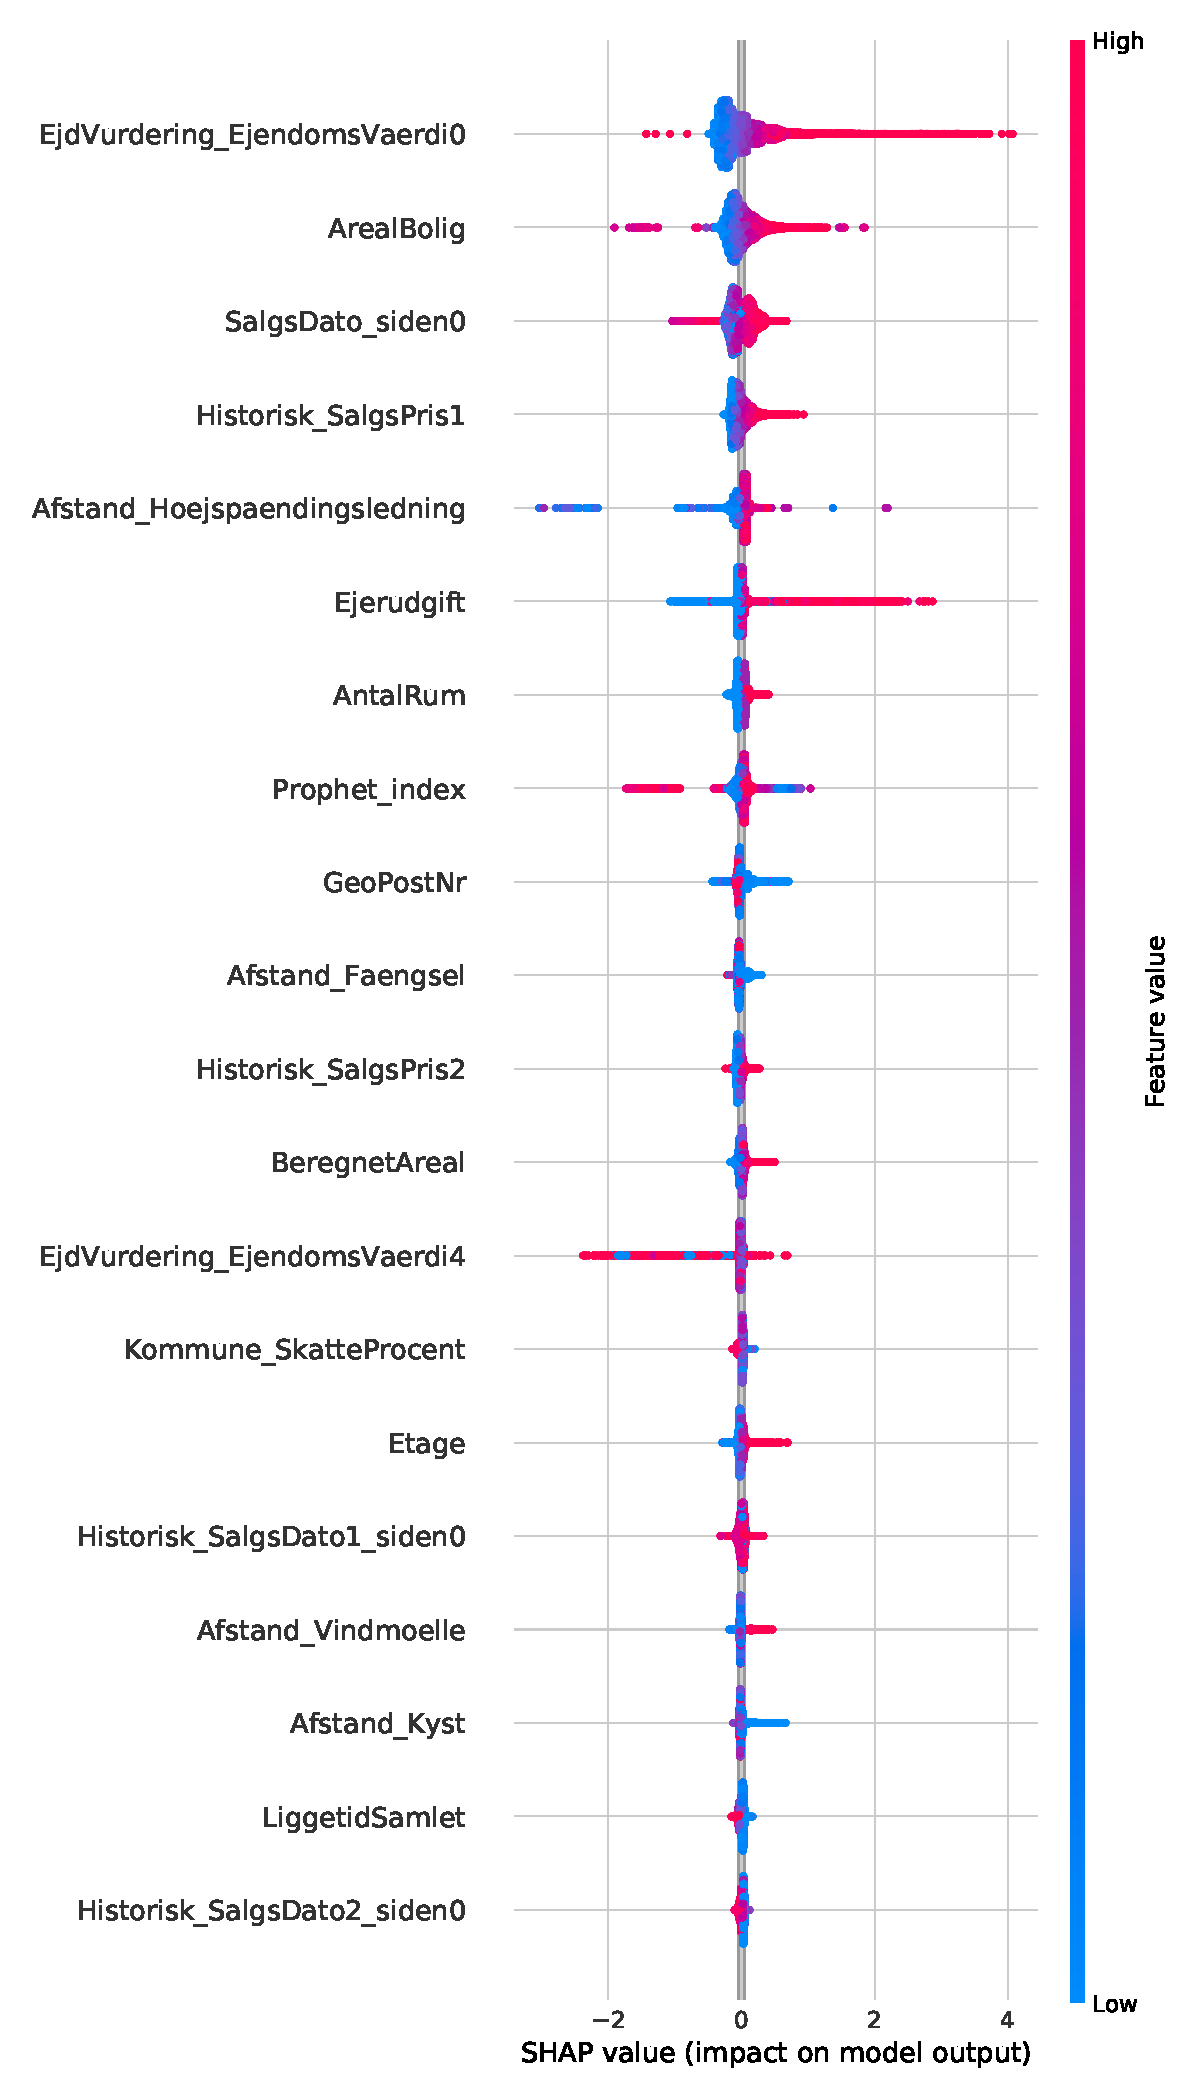
\includegraphics[width=0.9\textwidth, trim=0 0 0 1, clip]{figures/housing/Ejerlejlighed_v17_cut_all_Ncols_all_lgb_tight_SHAP_vals_summary.pdf}
  \caption[Feature importance of apartments prices using LGB][6pt]
          {Feature importance of apartment prices using the LGB-model. The feature importance is measured using SHAP values. The variables are sorted top to bottom according to their overall feature importance, i.e. the previous public property valuation \code{EjdVurdering_EjendomdsVaerdi0} is the most important single feature. Along the x-axis is the impact on model output, in this example the price in XXX. This axes is colored by the value of the feature, from \textcolor{blue}{low} (blue) to \textcolor{red}{high} (red). In this particular example we see that high values of the previous public property valuation has high, positive impact on the model prediction -- exactly as expected. This is exactly opposite the total days on market (DOM) described by the variable \code{LiggetidSamlet} where a high value has a negative impact.  
          } 
  \label{fig:h:shap_overview}
\end{figure}

\begin{figure}
  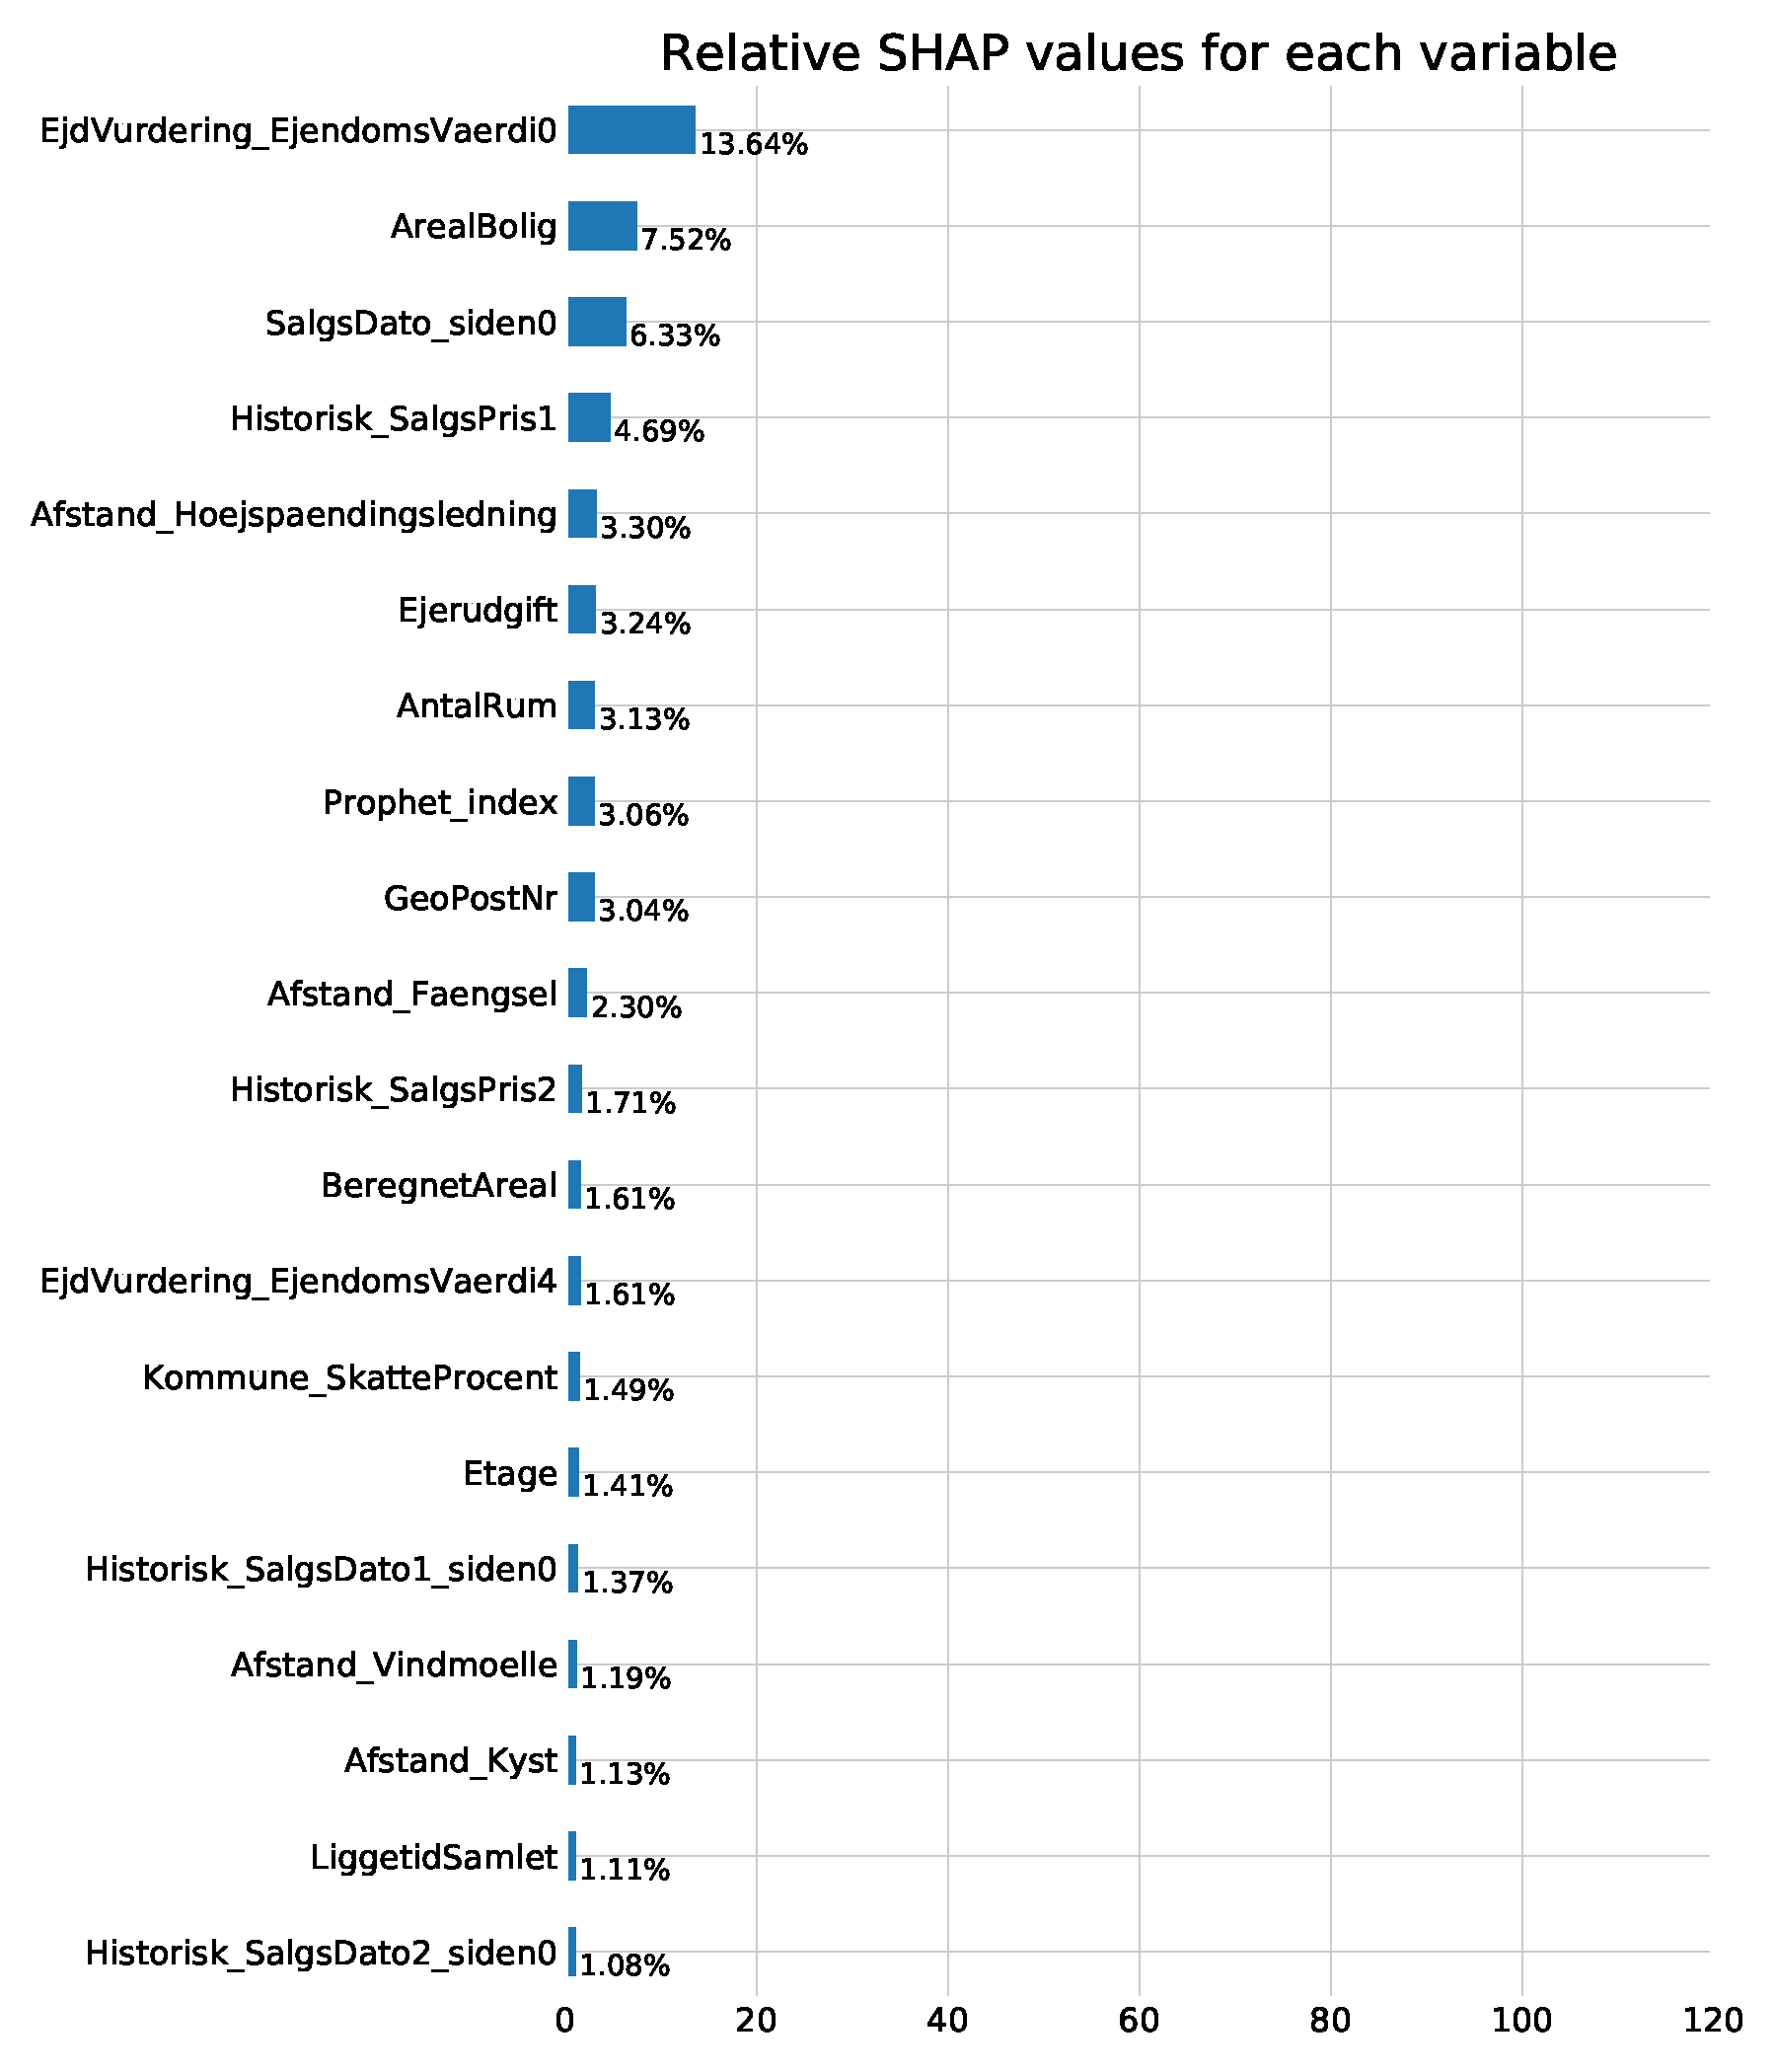
\includegraphics[width=0.9\textwidth, trim=0 0 0 40, clip]{figures/housing/Ejerlejlighed_v17_cut_all_Ncols_all_lgb_tight_SHAP_vals_summary_all.pdf}
  \caption[Total feature importance of apartment prices using LGB][6pt]
          {Total feature importance of apartment prices using the LGB-model. The total feature importance is measured using SHAP values, more specifically the mean of the absolute SHAP values for each variable. This allows a ranking of all of the features ordered after the total importance. Here the total feature importance is scaled such that they sum to 1 when summing over all variables. The absolute total feature importance is in itself not important, but the relative values indicate the difference in feature importance. 
          } 
  \label{fig:h:shap_overview_total}
\end{figure}


\begin{figure}
  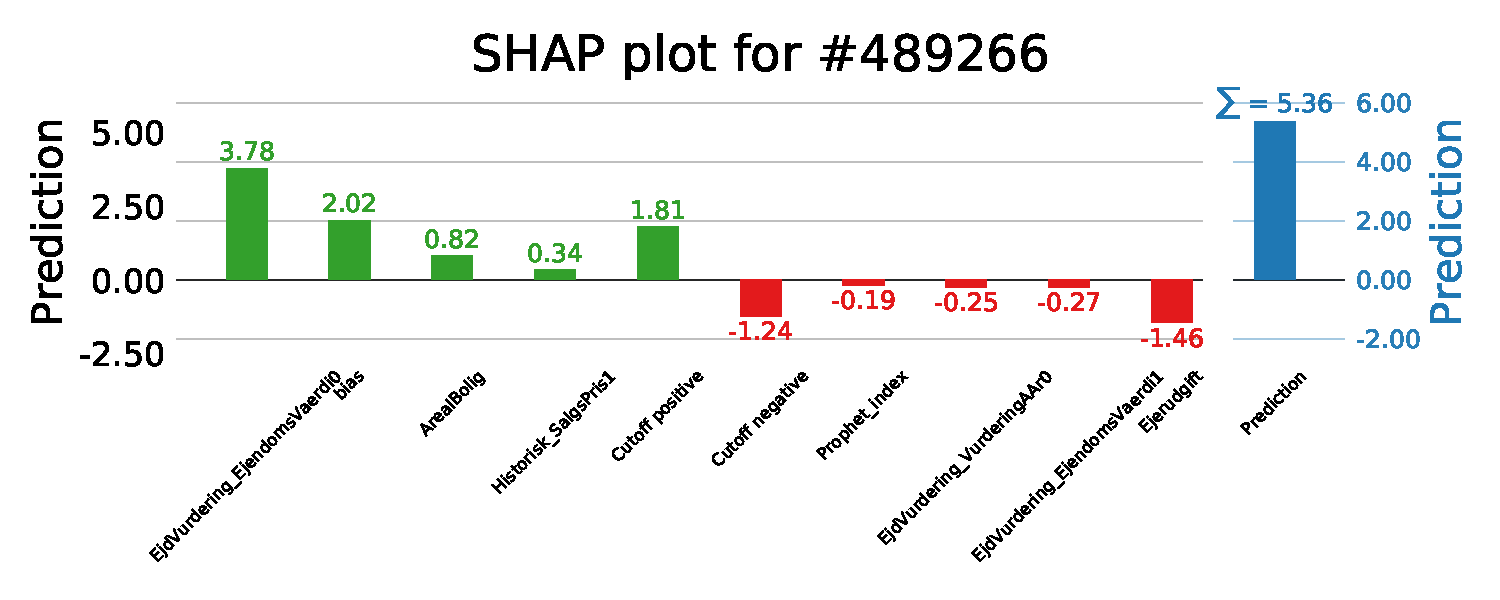
\includegraphics[width=0.95\textwidth, trim=0 0 0 40, clip]{figures/housing/Ejerlejlighed_v17_cut_all_Ncols_all_SHAP_fig_loc=489266.pdf}
  \caption[SHAP Prediction Explanation for apartment][6pt]
          {Model explanation for LGB model for a specific apartment. The bars are the variables in the dataset that the model found most important sorted after their importance for this particular apartment. The bias bar refers to the expected value of the model, which is simply the mean of the training set which acts as the naive prediction baseline. The \q{cutoff positive (negative)} bars are the sum of the remaining positive (negative) values that are not shown. On the right hand side of the plot is the model prediction shown. The model prediction is the sum of all of the bars in the left par (5.36 in this example) calculated in $10^6$ DKK. The \textcolor{red}{negative} values are shown in red, \textcolor{green}{positive} ones in green, and the \textcolor{blue}{prediction value} in blue. 
          } 
  \label{fig:h:shap_single_apartment}
\end{figure}


\begin{figure}
  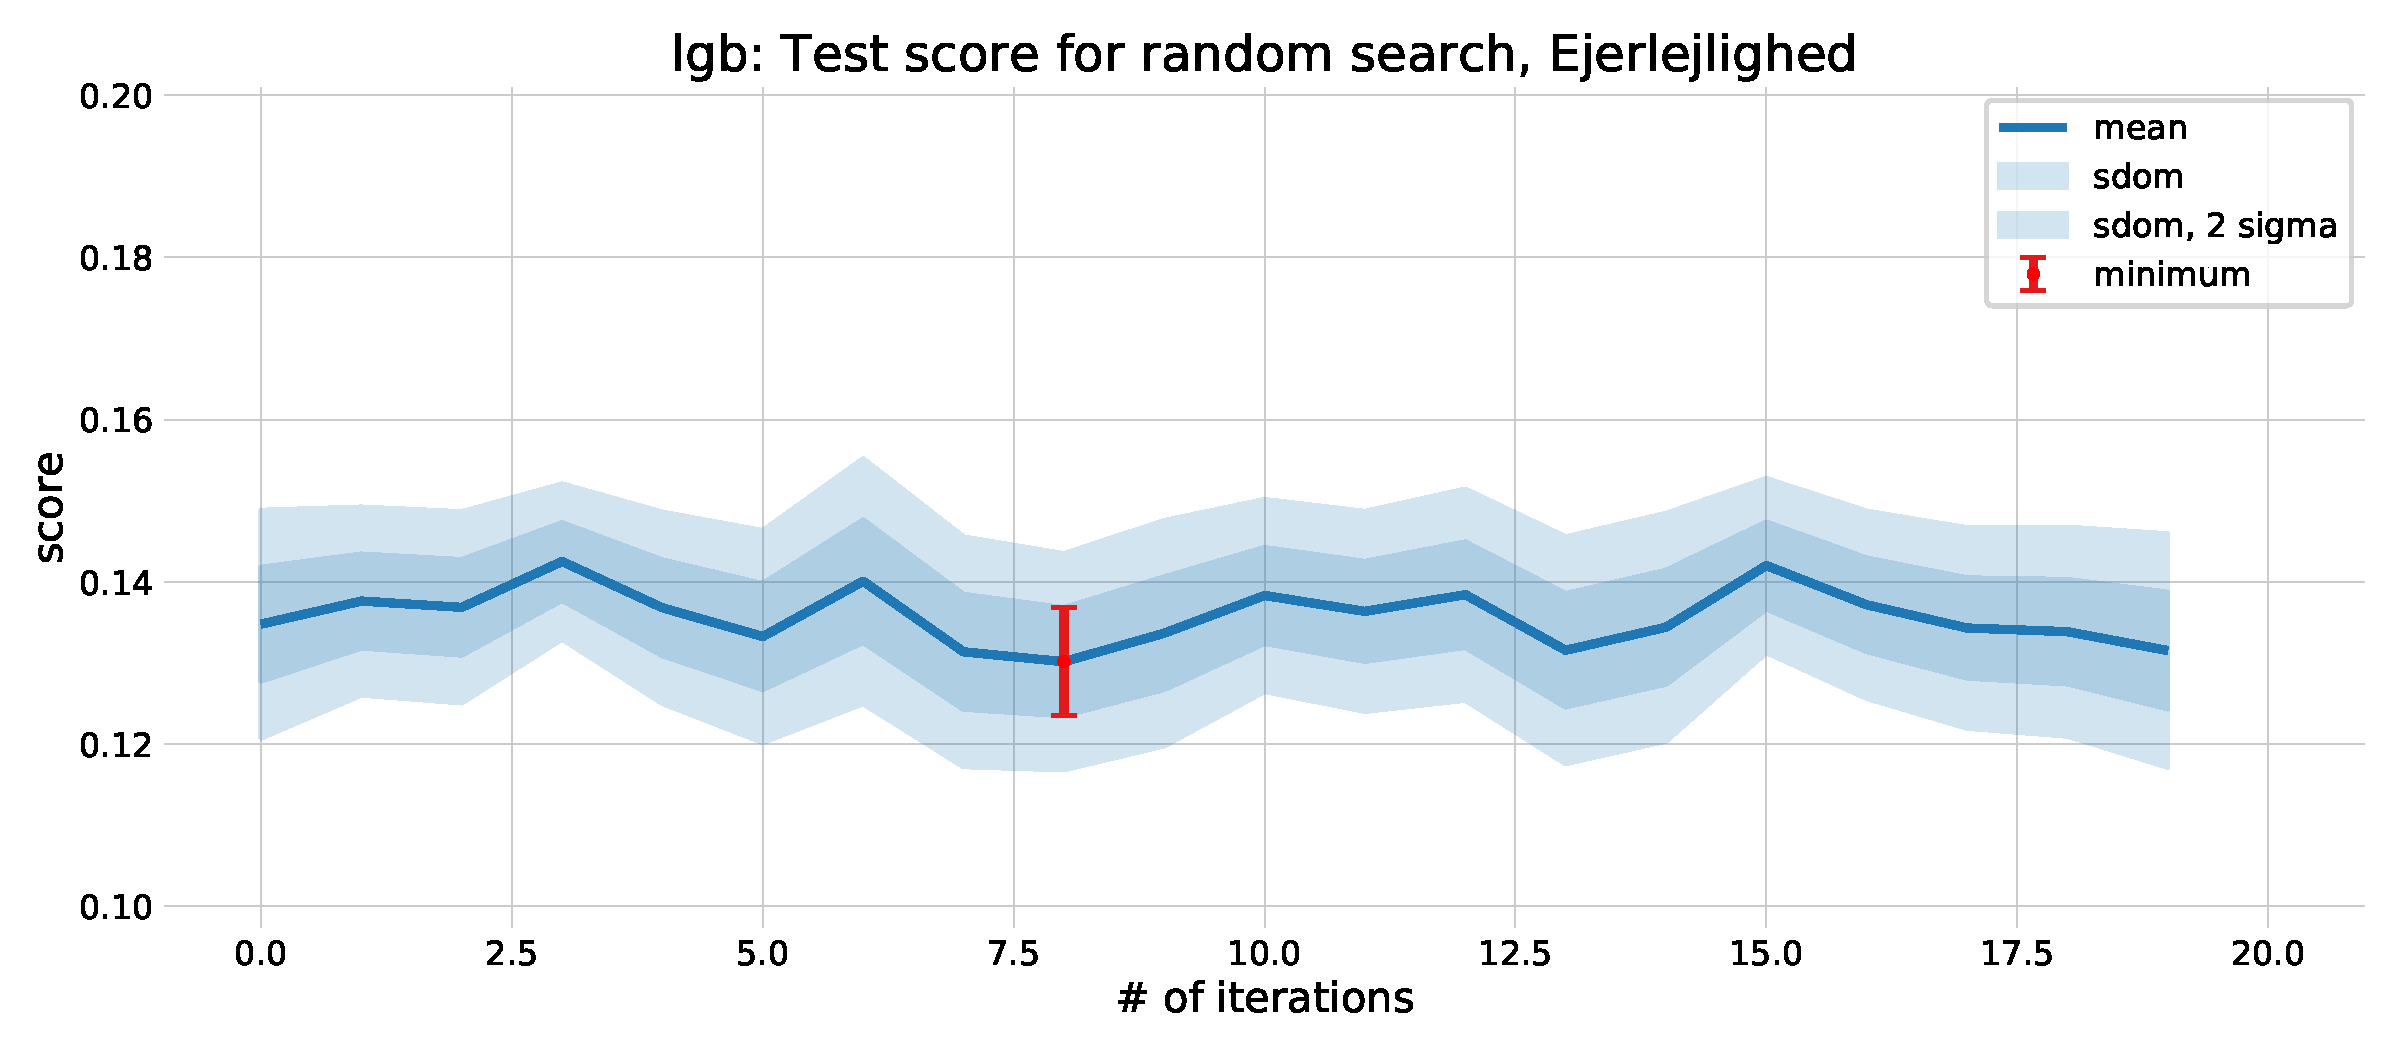
\includegraphics[width=0.9\textwidth, trim=0 0 0 40, clip]{figures/housing/Ejerlejlighed_v17_cut_all_Ncols_all_lgb_score_over_time_random.pdf}
  \caption[Hyperparameter optimization: random search results][6pt]
          {The results of running random search (RS) as hyperparameter optimization (HPO) on apartments using the LGB-model. The \textcolor{red}{minimum (mean) loss} along with its uncertainty is shown in red, the \textcolor{blue}{means} for the different iterations of RS in blue, and as light blue bands are the \textcolor{blue}{one (and two) standard deviation(s) of the means (SDOM)}, all as a a function of iteration number.  
          } 
  \label{fig:h:RS_lgb_apartment}
\end{figure}


\begin{figure}
  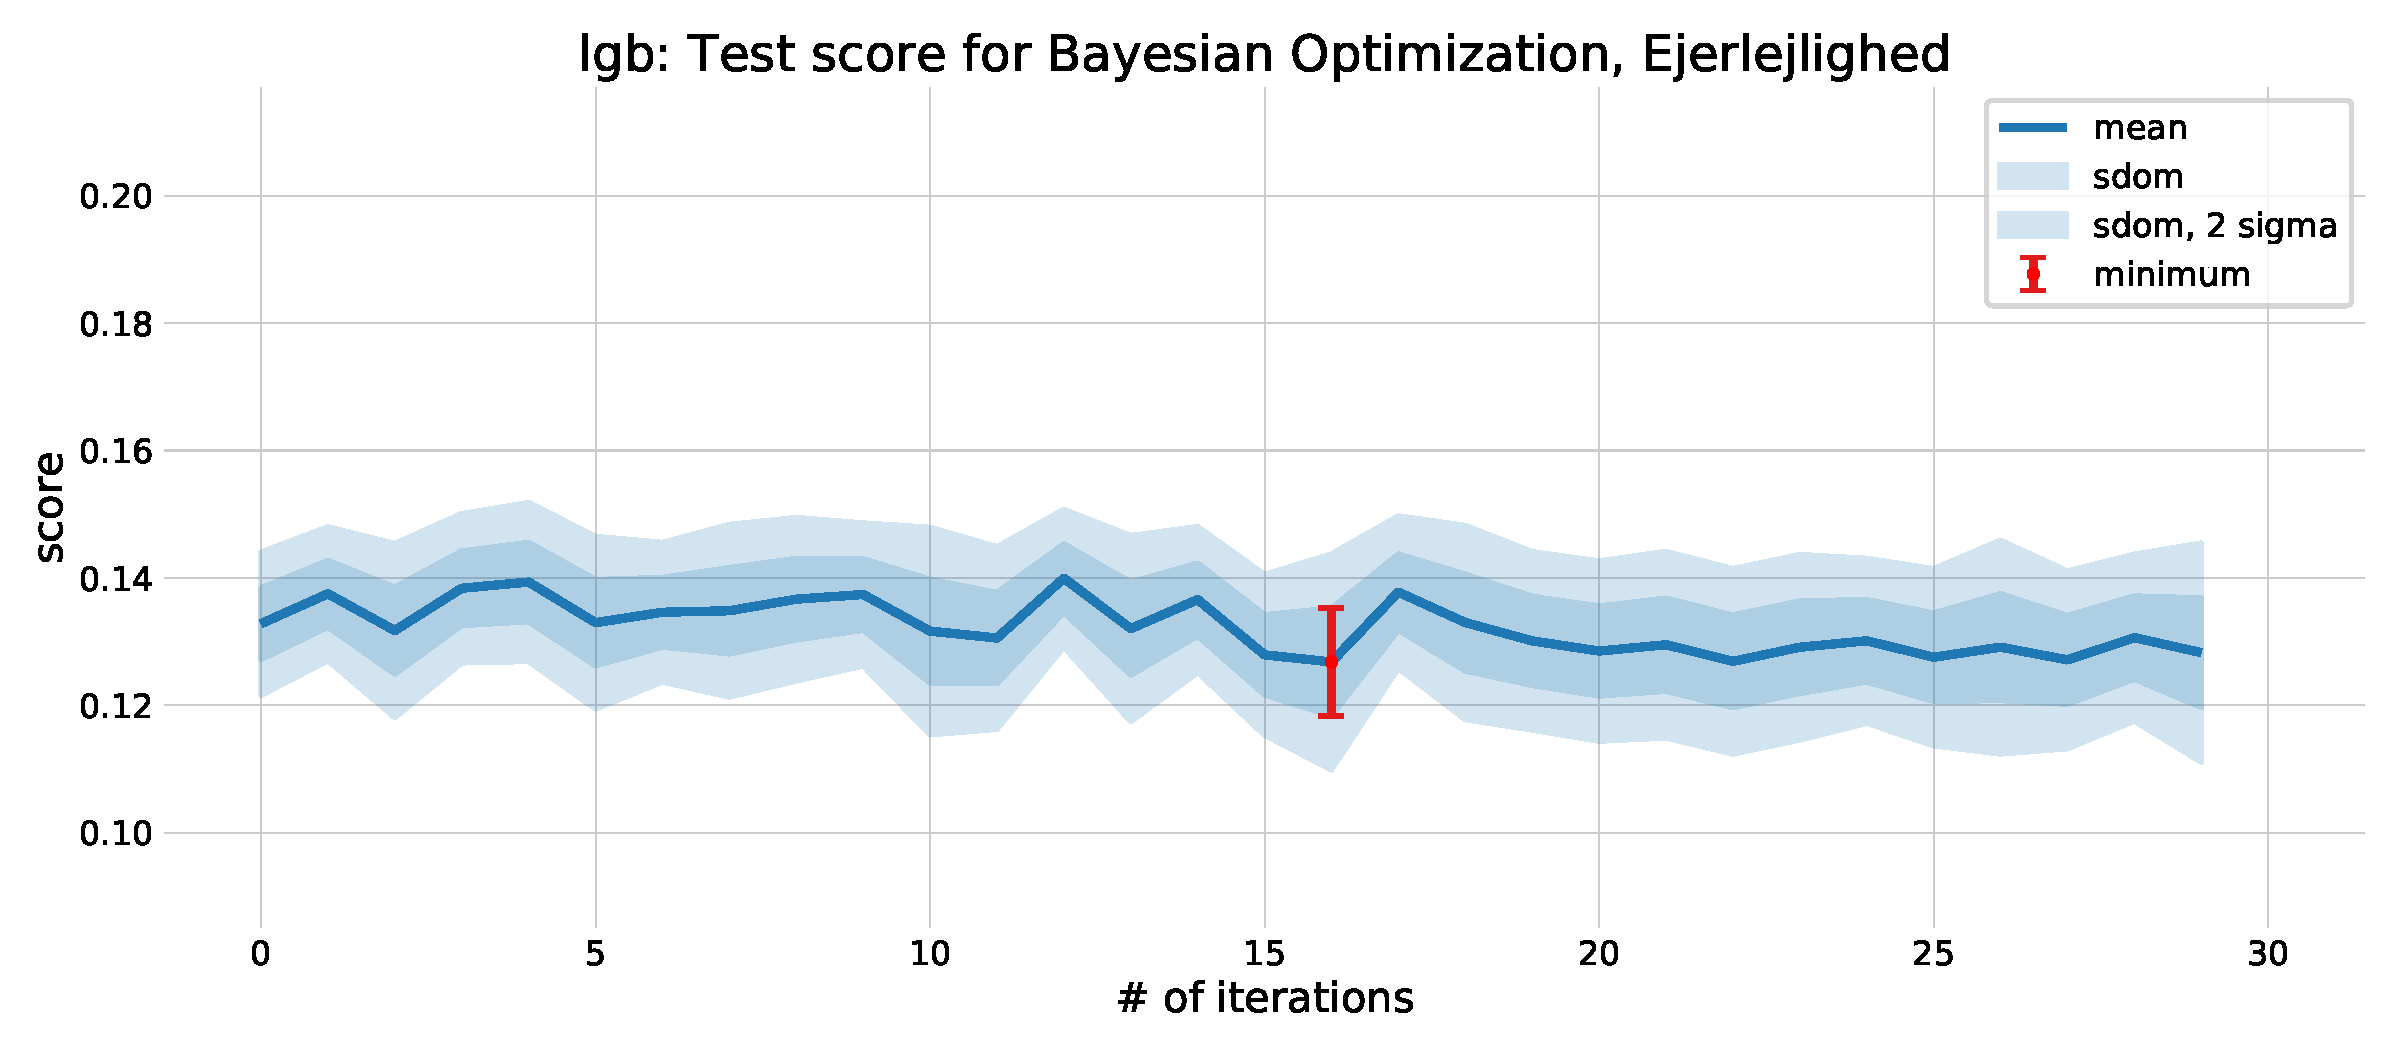
\includegraphics[width=0.9\textwidth, trim=0 0 0 40, clip]{figures/housing/Ejerlejlighed_v17_cut_all_Ncols_all_lgb_score_over_time_BO.pdf}
  \caption[Hyperparameter optimization: Bayesian optimization results][6pt]
          {The results of running Bayesian optimization (BO) as hyperparameter optimization (HPO) on apartments using the LGB-model. The \textcolor{red}{minimum (mean) loss} along with its uncertainty is shown in red, the \textcolor{blue}{means} for the different iterations of RS in blue, and as light blue bands are the \textcolor{blue}{one (and two) standard deviation(s) of the means (SDOM)}, all as a a function of iteration number. The first XXX iterations are run as RS for use as input to the internal optimization algorithm, the last XX iterations are thus the \q{smart} BO guesses.
          } 
  \label{fig:h:BO_lgb_apartment}
\end{figure}


\begin{figure}
  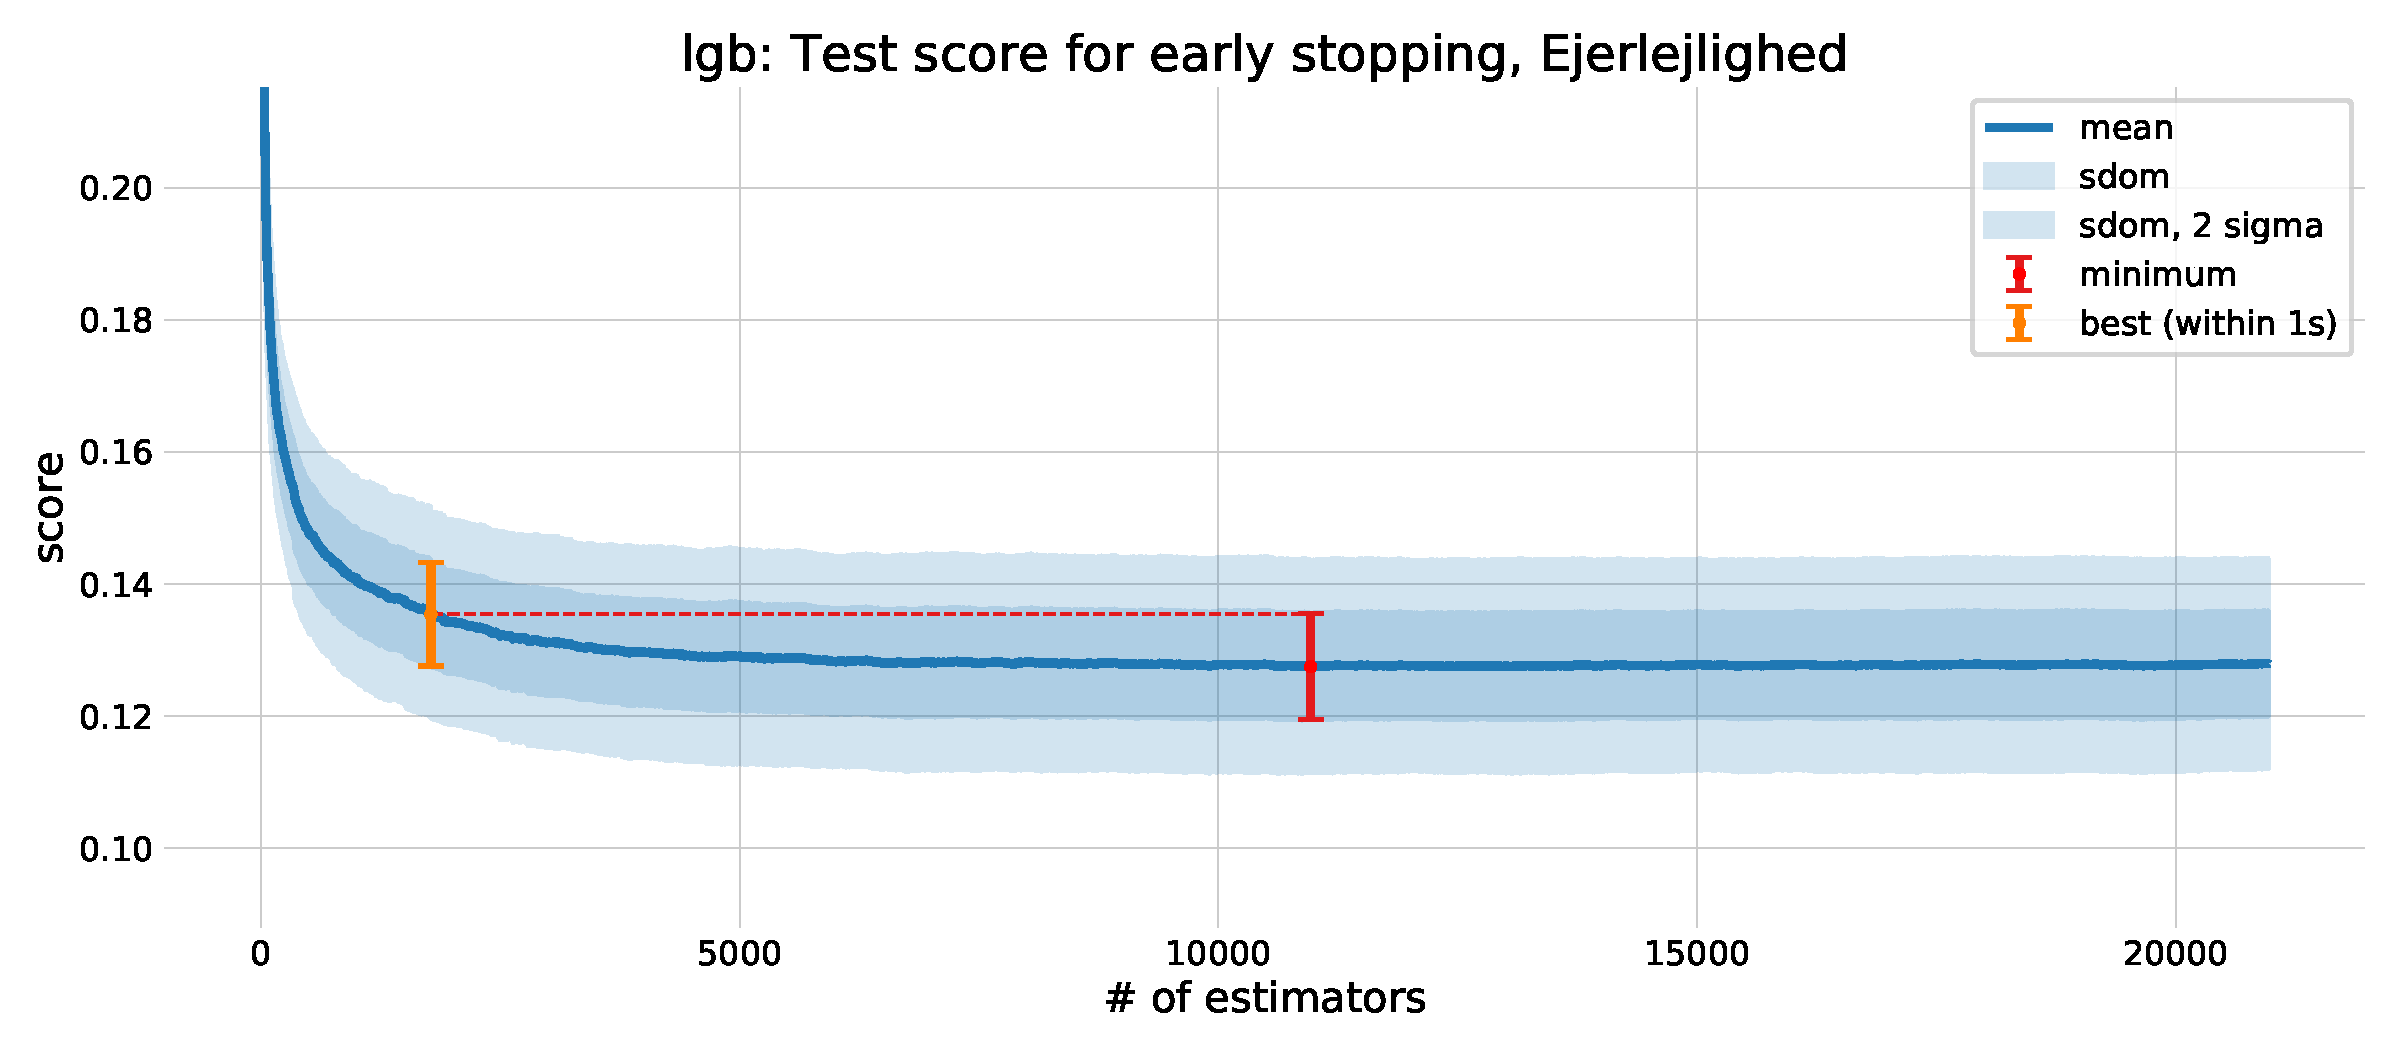
\includegraphics[width=0.9\textwidth, trim=0 0 0 40, clip]{figures/housing/Ejerlejlighed_v17_cut_all_Ncols_all_lgb_early_stopping_fig.pdf}
  \caption[Early Stopping results][6pt]
          {The results of early stopping on apartments using the LGB-model. The \textcolor{red}{minimum (mean) loss} along with its uncertainty is shown in red, the \textcolor{blue}{means} for the different iterations of RS in blue, and as light blue bands are the \textcolor{blue}{one (and two) standard deviation(s) of the means (SDOM)}, all as a a function of number of estimators (trees). In orange the \textcolor{orange}{\q{best} number of estimators} is shown, defined as the lowest number of estimators which are still within 1 SDOM of the minimum value. This leads to a model that has a performance that is within 1 SDOM of the best model, but a lot simpler and faster.  
          } 
  \label{fig:h:early_stopping}
\end{figure}


\begin{figure}
  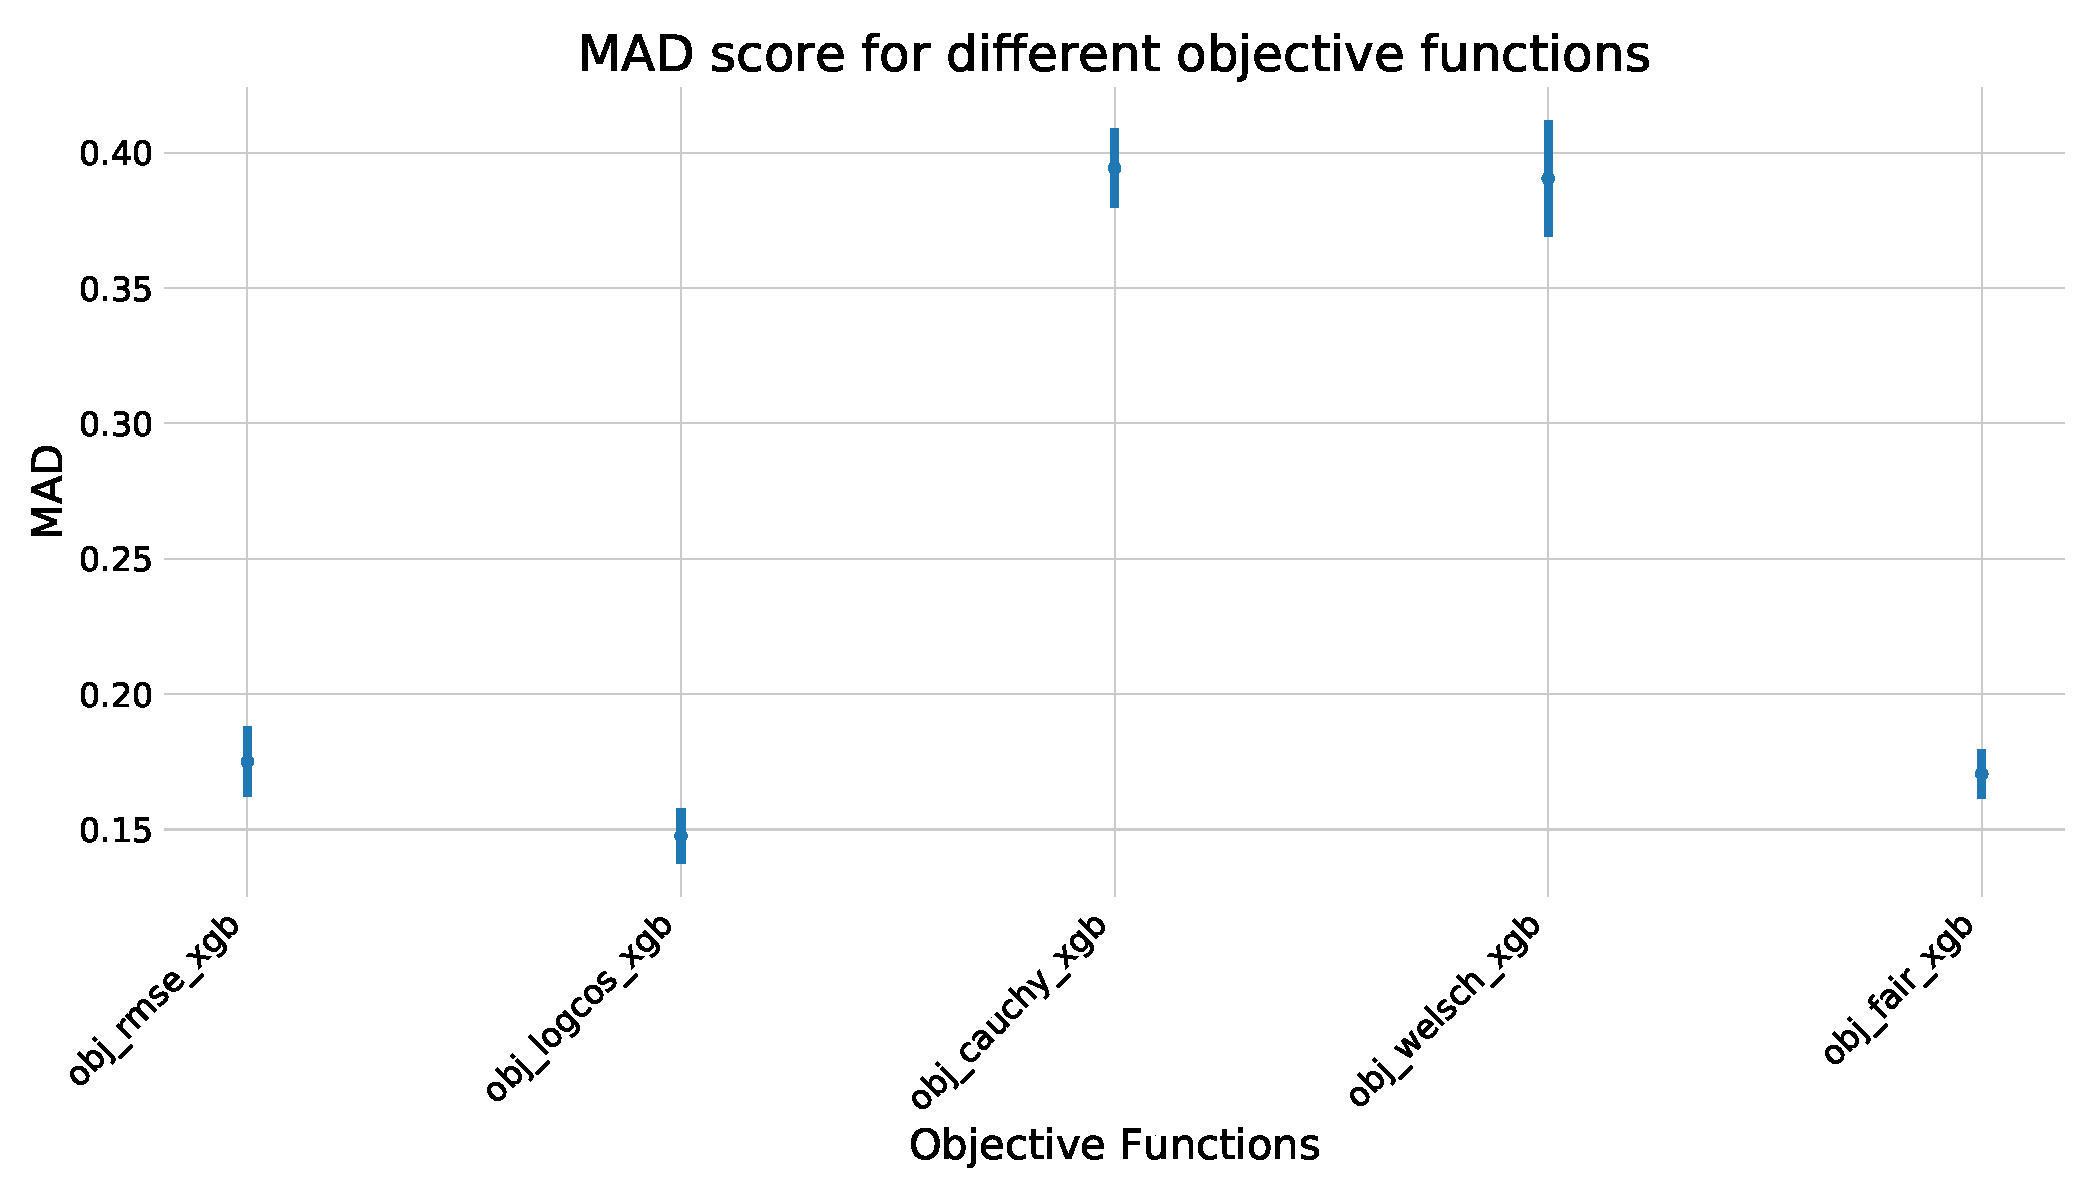
\includegraphics[width=0.9\textwidth, trim=0 35 0 40, clip]{figures/housing/Ejerlejlighed_v17_cut_all_Ncols_all__MAD_gridsearch_obj.pdf}
  \caption[Comparison of different objective functions][6pt]
          {Comparison of performance (measured using the median of the absolute deviation, MAD, for apartments) of the five different objective functions: RMSE, LogCosh, Cauchy, Welsch, and Fair. We see that the default objective function, RMSE, does a reasonable job, however, the LogCosh function is a clear improvement.
          } 
  \label{fig:h:objective_functions_performance}
\end{figure}



\begin{figure}
  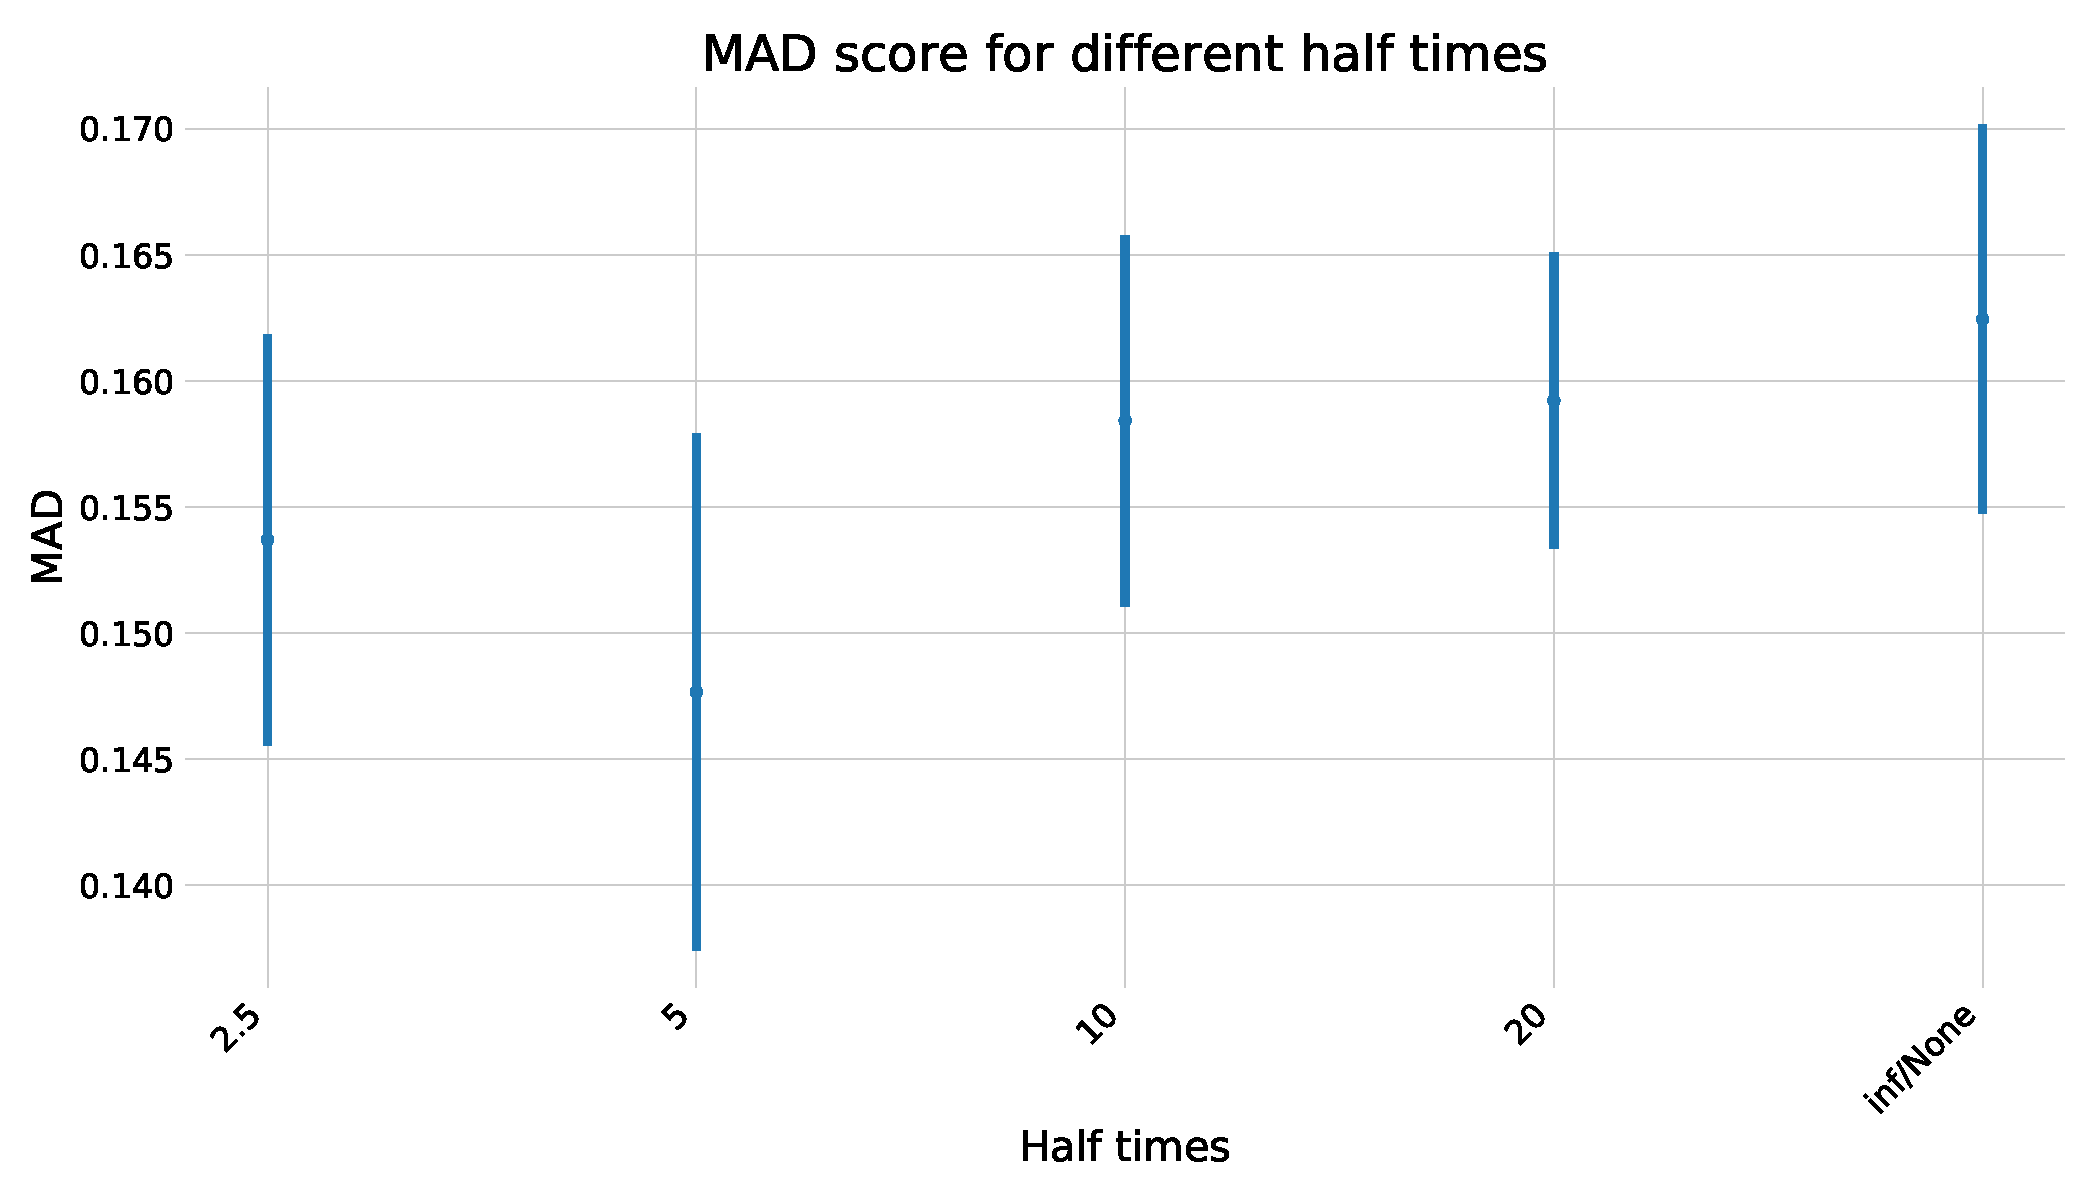
\includegraphics[width=0.9\textwidth, trim=0 0 0 40, clip]{figures/housing/Ejerlejlighed_v17_cut_all_Ncols_all__MAD_gridsearch_half.pdf}
  \caption[Comparison of different half times weights][6pt]
          {Comparison of performance (measured using the median of the absolute deviation, MAD, on apartments) of the five different half time weights: 2.5, 5, 10, 20, inf/None. We see that using no half time weights does has the worst performance, whereas a 5-year half time weight has the best performance (although with a very high uncertainty).
          } 
  \label{fig:h:half_time_performance}
\end{figure}



\begin{figure}
  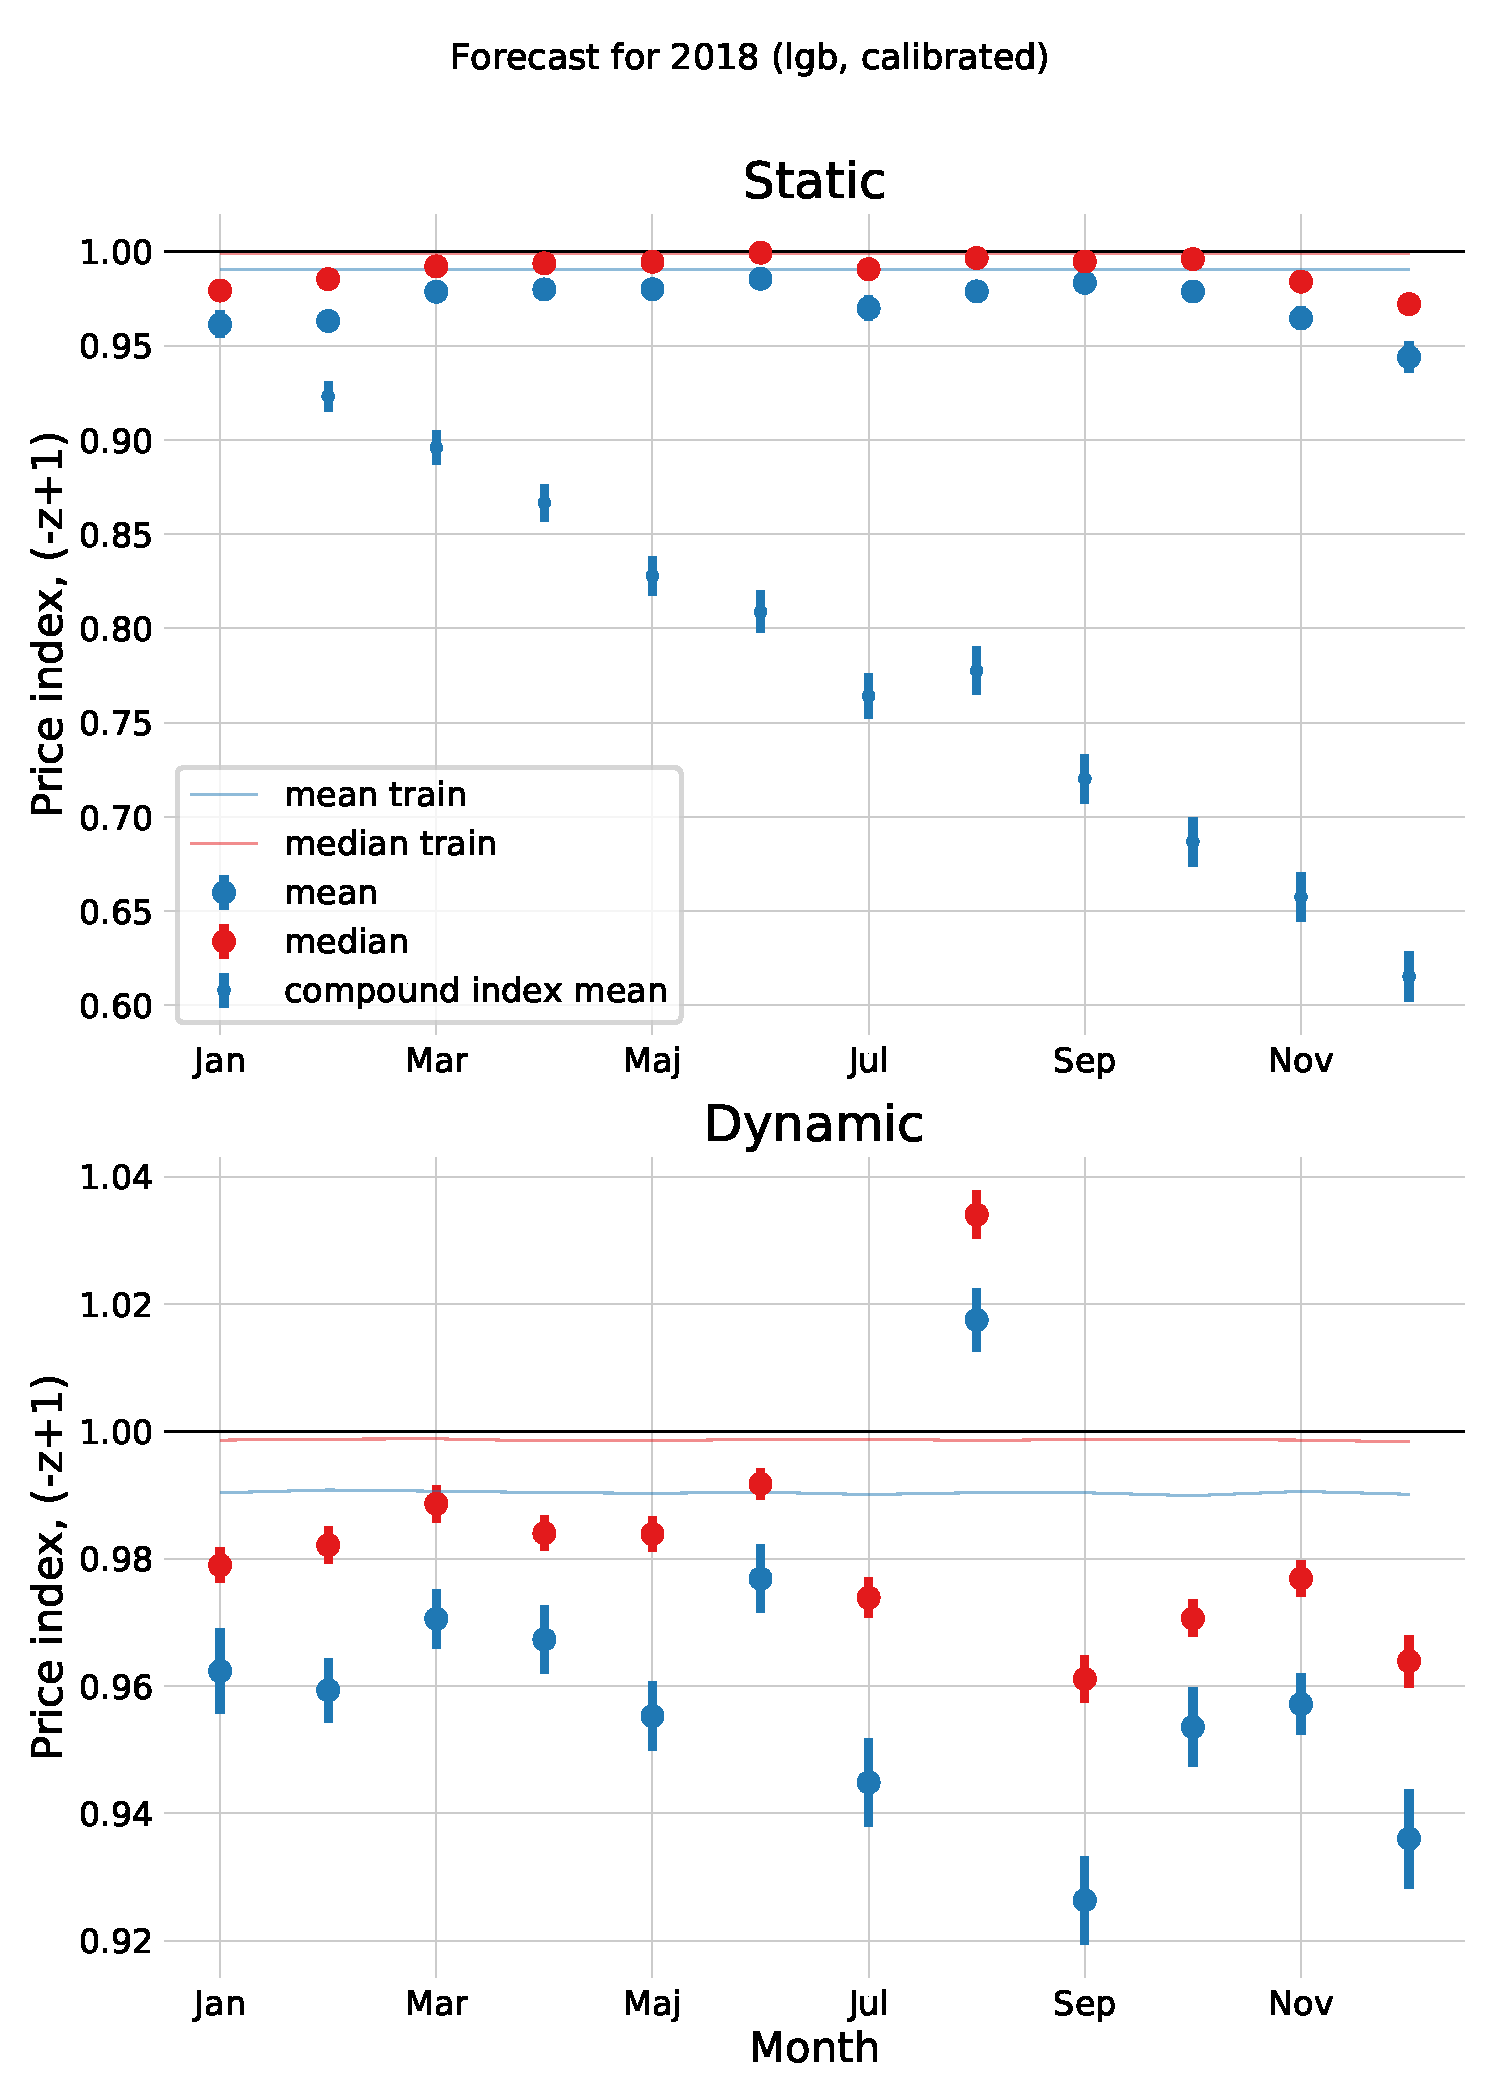
\includegraphics[width=0.9\textwidth, trim=0 0 0 70, clip]{figures/housing/Ejerlejlighed_v17_cut_all_Ncols_all__lgb_forecast_prediction_2018.pdf}
  \caption[2018 LGB Forecast][6pt]
          {Performance of 1-month forecasts for 2018 for apartments. For both plots the LGM model is trained on data up to (but excluding) 2018. Top) The performance of the static model's prediction on sales in the individual months of 2018 is shown for both the \textcolor{blue}{mean} and \textcolor{red}{median} of the $z$-scores. Bottom) Same as above, however this time based a dynamic model, i.e. a model which is retrained after every month to include the previous month's sales.
          } 
  \label{fig:h:forecast_2018_lgb}
\end{figure}









\section{Headings}\label{sec:headings1}\index{headings}

Tufte's books include the following heading levels: parts,
chapters,\sidenote{Parts and chapters are defined for the \texttt{tufte-book}
class only.}  sections, subsections, and paragraphs.  Not defined by default
are: sub-subsections and subparagraphs.

\begin{table}[h]
  \begin{center}
    \footnotesize%
    \begin{tabular}{lcr}
      \toprule
      Heading & Style & Size \\
      \midrule
      Part & roman & \measure{24}{36}{40} \\
      Chapter & italic & \measure{20}{30}{40} \\
      Section & italic & \measure{12}{16}{26} \\
      Subsection & italic & \measure{11}{15}{26} \\
      Paragraph & italic & 10/14 \\
      \bottomrule
    \end{tabular}
  \end{center}
  \caption{Heading styles used in \BE.}
  \label{tab:heading-styles}
\end{table}

\paragraph{Paragraph} Paragraph headings (as shown here) are introduced by
italicized text and separated from the main paragraph by a bit of space.

\chapter{Particle Physics and LEP}
\label{ch:particle_physcis_LEP}
% \immediate\write{./quote.sh \the\value{chapter}}
% \epigraph{\input{/tmp/fortune-\the\value{chapter}}}{--- \textup{\texttt{/usr/bin/fortune}}}


\begin{figure}
  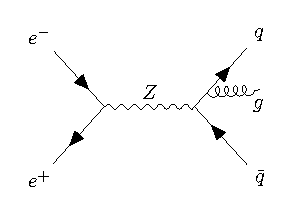
\includegraphics[width=0.9\textwidth]{figures/feynman_diagrams/eeZqqg.pdf}
  \caption[Feynman diagram for the jet production at LEP][6pt]{Feynman diagram showing the $e^+ e^- \rightarrow Z^0$ production at LEP. The $Z^0$ has several decay modes where the $Z \rightarrow q\bar{q}g$ is shown here.}
  \label{fig:hep:feynman_3j_qqg}
  %\zsavepos{pos:textfig}
\end{figure}






The \TL document classes define a style similar to the
style Edward Tufte uses in his books and handouts.  Tufte's style is known
for its extensive use of sidenotes, tight integration of graphics with
text, and well-set typography.  This document aims to be at once a
demonstration of the features of the \TL document classes
and a style guide to their use.

\section{Page Layout}\label{sec:page-layout}
\subsection{Headings}\label{sec:headings}\index{headings}
This style provides \textsc{a}- and \textsc{b}-heads (that is,
\Verb|\section| and \Verb|\subsection|), demonstrated above.

If you need more than two levels of section headings, you'll have to define
them yourself at the moment; there are no pre-defined styles for anything below
a \Verb|\subsection|.  As Bringhurst points out in \textit{The Elements of
Typographic Style}, 
%  \citep{Bringhurst2005} 
you should ``use as many levels of
headings as you need: no more, and no fewer.''

The \TL classes will emit an error if you try to use
\linebreak\Verb|\subsubsection| and smaller headings.

% let's start a new thought -- a new section
\newthought{In his later books}, 
%  \citep{Tufte2006}
 Tufte
starts each section with a bit of vertical space, a non-indented paragraph,
and sets the first few words of the sentence in \textsc{small caps}.  To
accomplish this using this style, use the \doccmddef{newthought} command:
\begin{docspec}
  \doccmd{newthought}\{In his later books\}, Tufte starts\ldots
\end{docspec}



\chapter{Quark Gluon Analysis}
\label{ch:quark_gluon_analysis}

\section{Sidenotes}\label{sec:sidenotes}
One of the most prominent and distinctive features of this style is the
extensive use of sidenotes.  There is a wide margin to provide ample room
for sidenotes and small figures.  Any \doccmd{footnote}s will automatically
be converted to sidenotes.\footnote{This is a sidenote that was entered
using the \texttt{\textbackslash footnote} command.}  If you'd like to place ancillary
information in the margin without the sidenote mark (the superscript
number), you can use the \doccmd{marginnote} command.\marginnote{This is a
margin note.  Notice that there isn't a number preceding the note, and
there is no number in the main text where this note was written.}





\begin{figure}
  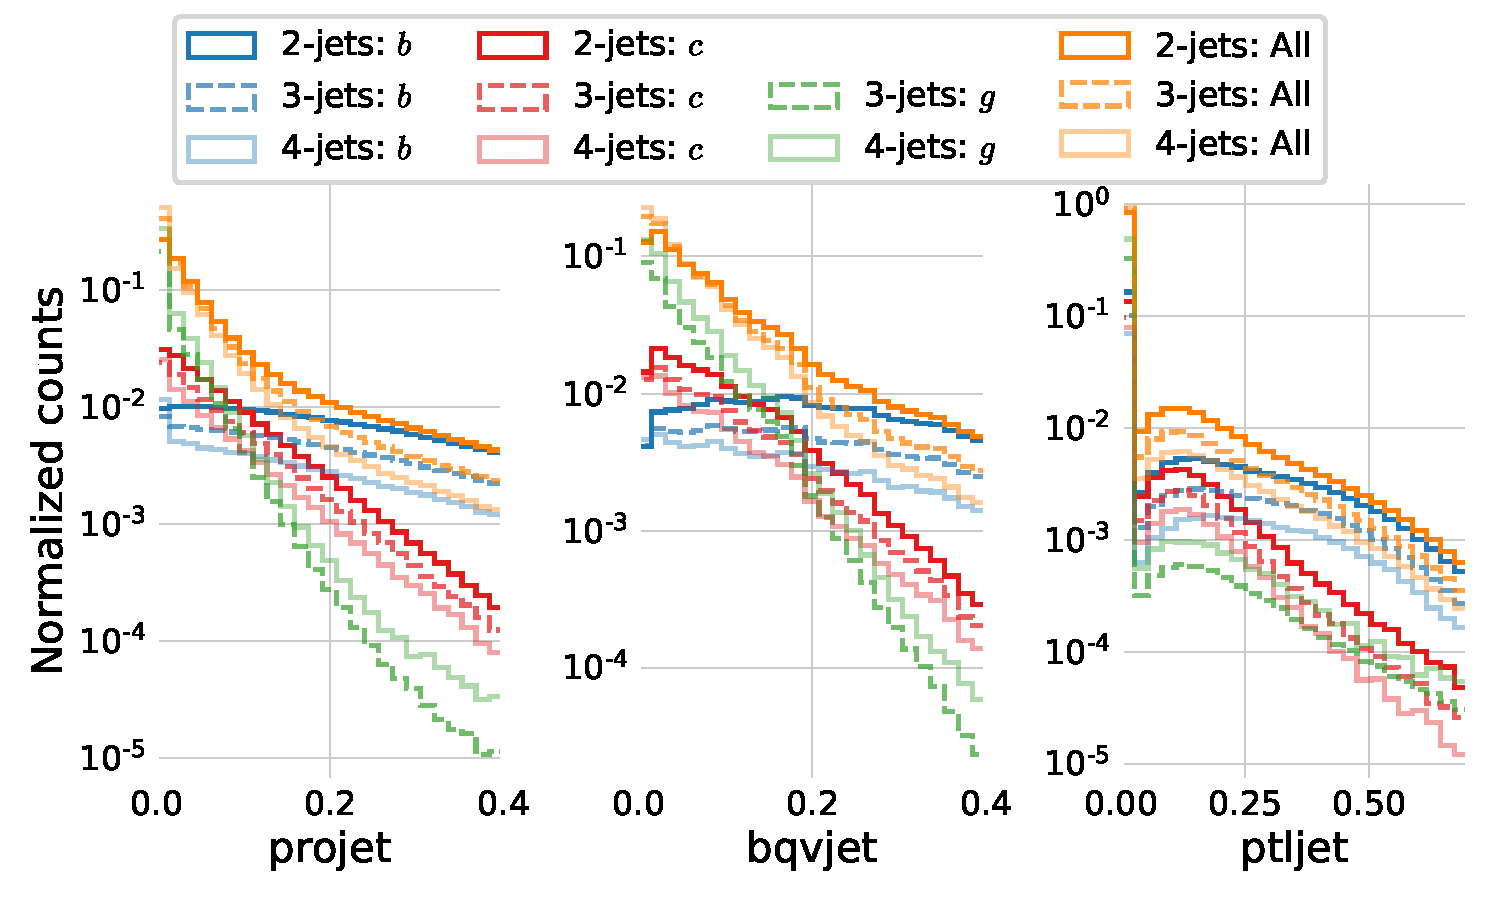
\includegraphics[width=0.95\textwidth, trim=0 0 0 0, clip]{figures/quarks/btagging_variables_hist-down_sample=1.00-ML_vars=vertex-selection=b-ejet_min=4-n_iter_RS_lgb=99-n_iter_RS_xgb=9-cdot_cut=0.90-version=19.pdf}
  \caption[Histograms of the vertex variables][6pt]
          {Histograms of the three vertex variables, \code{projet}, \code{bqvjet}, and \code{ptljet}, used as input variables in the b-tagging models. In blue colors the variables are shown for \textcolor{blue}{true b-jets}, in red for \textcolor{red}{true c-jets}, in green for \textcolor{green}{true g-jets}, and in orange for \textcolor{orange}{all of the jets} (including non q-matched). In fully opaque color are shown the distributions for 2-jet events, in dashed (and lighter color) 3-jet events, and in semi-transparent 4-jet events. Notice the logarithmic y-axis, that there are no g-jets for 2-jet events (as expected), and that all of the distributions are very similar not matter how many jets.
          } 
  \label{fig:q:vertex_variables}
\end{figure}



\begin{figure}
  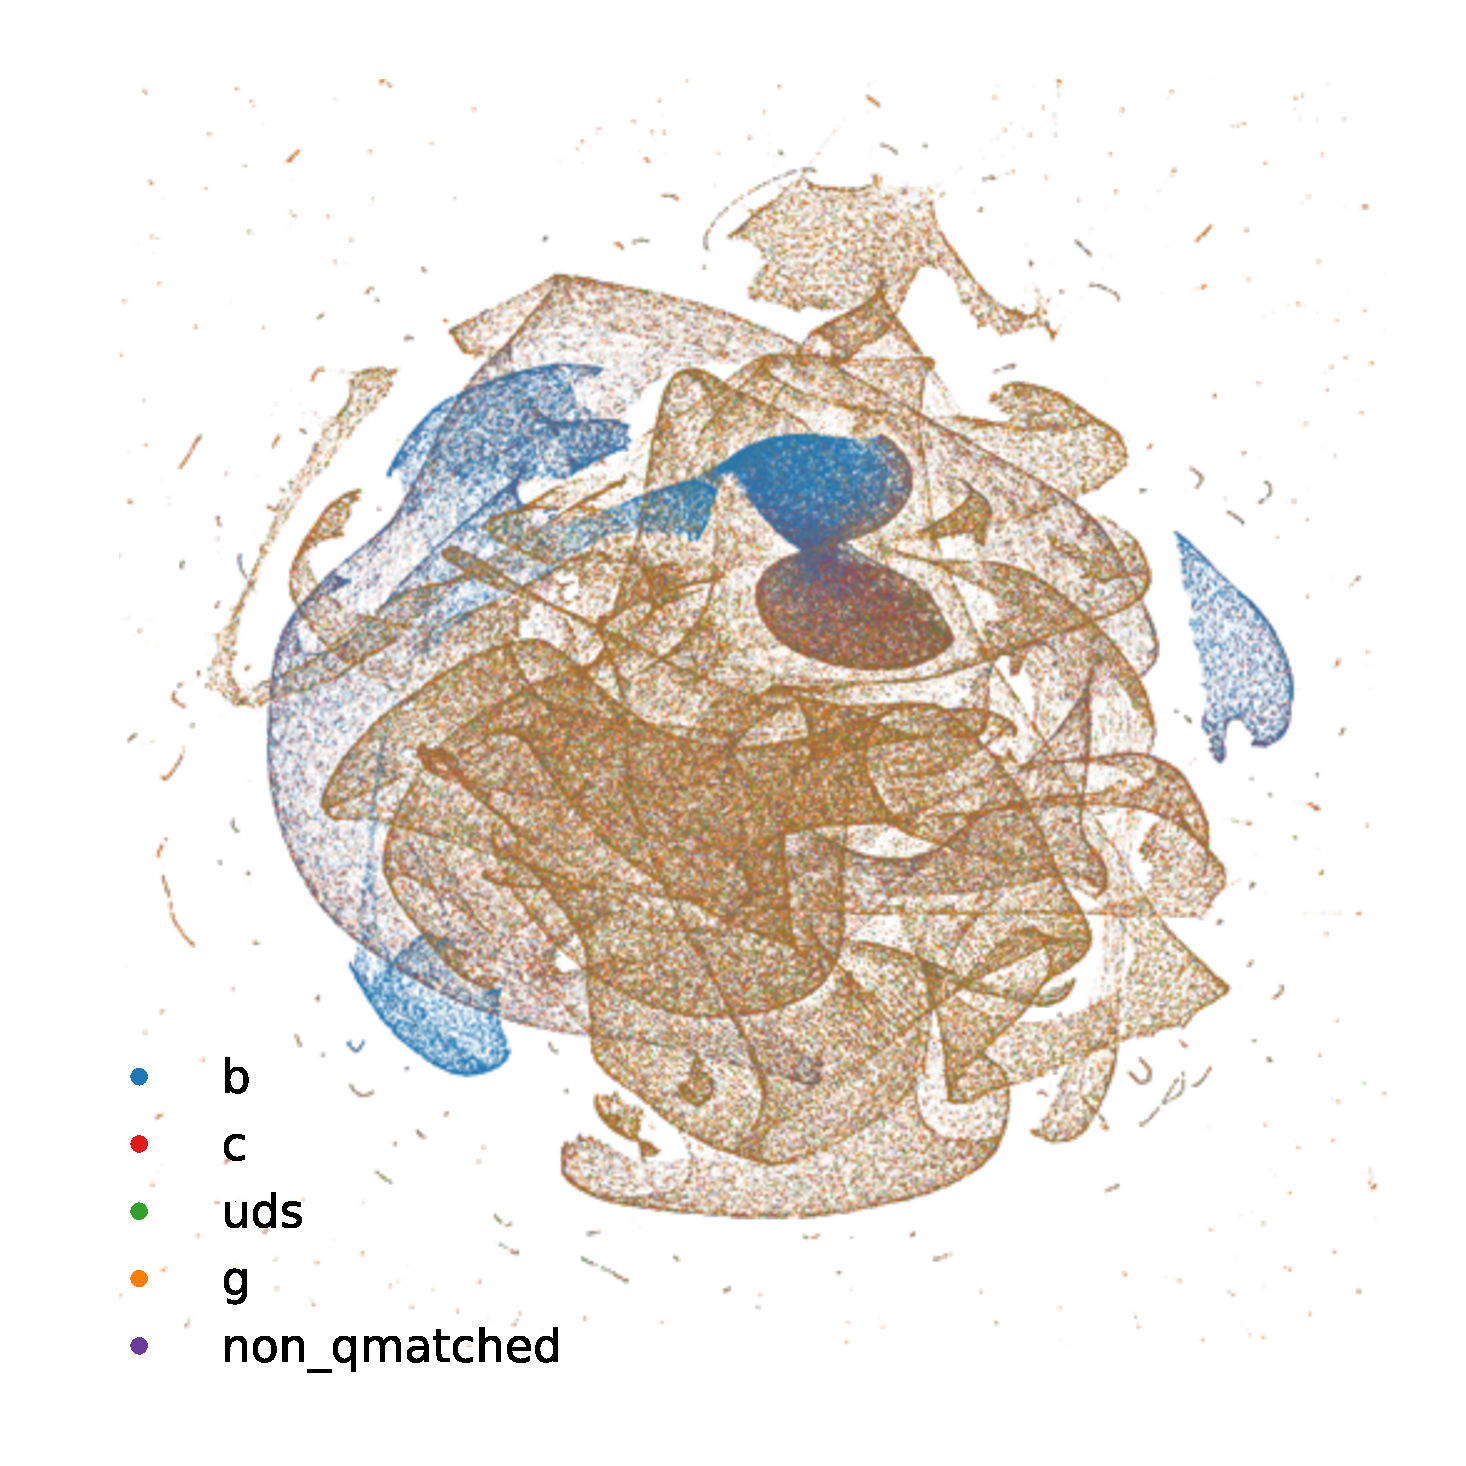
\includegraphics[width=0.95\textwidth, trim=20 20 50 50, clip]{figures/quarks/df_UMAP-X=1120952-n_neighbors=250-min_dist=0.2-metric=euclidean-input2b_njet=4_algorithm=UMAP_single.pdf}
  \caption[UMAP vizualisation of vertex variables][6pt]
          {Vizualisation of the vertex variables for the different categories: \textcolor{blue}{true b-jets} in blue, \textcolor{red}{true c-jets} in red, \textcolor{green}{true uds-jets} in green, \textcolor{orange}{true g-jets} in orange, and \textcolor{purple}{non q-matched}. The clustering is performed with the UMAP algorithm which outputs a 2D-projection. This projection is then visualized using the Datashader which takes takes care of point size, avoids over- and under-plotting, and color intensity. 
          } 
  \label{fig:q:UMAP_vertex}
\end{figure}



\begin{figure}
  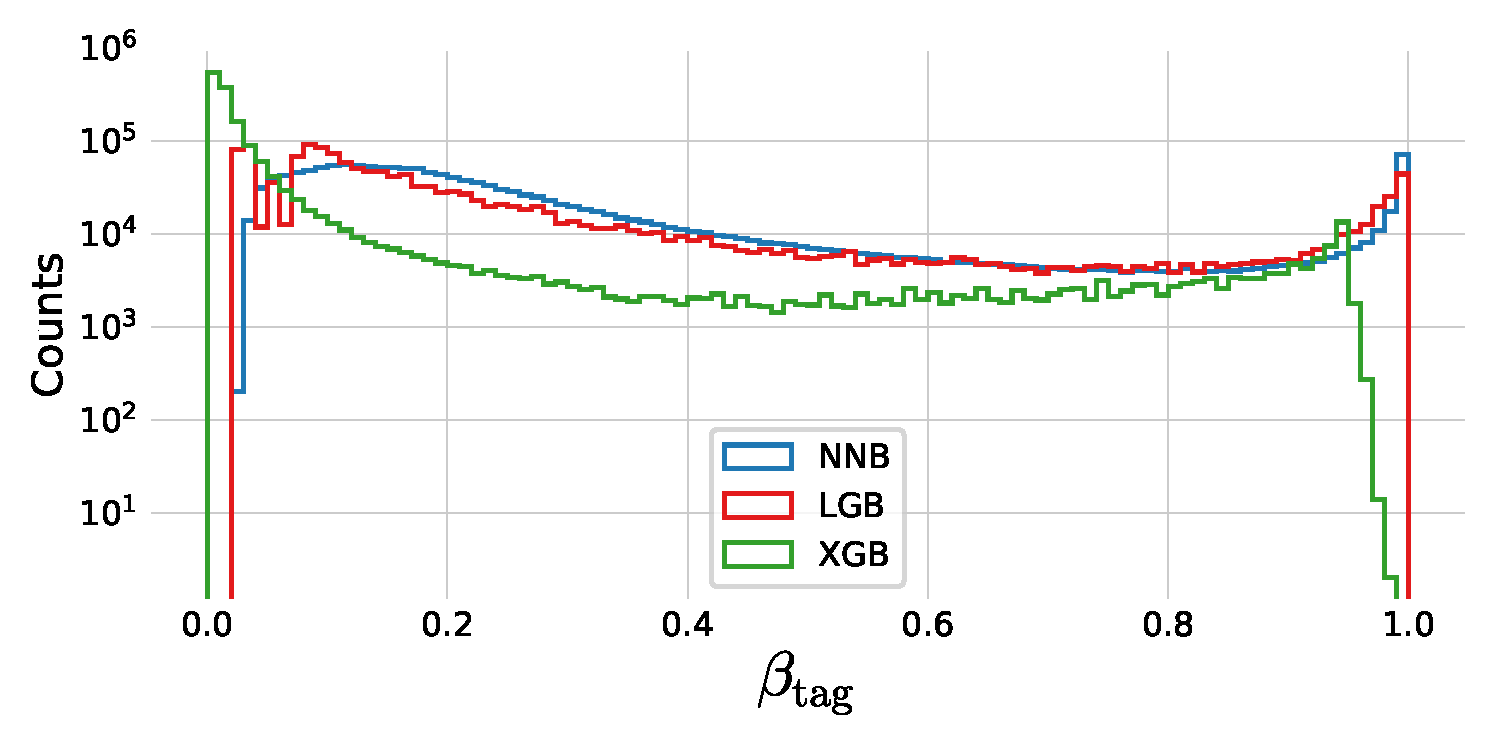
\includegraphics[width=0.95\textwidth, trim=0 0 0 30, clip]{figures/quarks/y_pred_3_jet_hist-down_sample=1.00-ML_vars=vertex-selection=b-ejet_min=4-n_iter_RS_lgb=99-n_iter_RS_xgb=9-cdot_cut=0.90-version=19.pdf}
  \caption[b-tag scores in 3-jet events][6pt]
          {Histogram of b-tag scores (model prediction) in 3-jet events for \textcolor{blue}{NNB} (the neural network trained by ATLAS, also called \code{nnbjet}) in blue, \textcolor{red}{LGB} in red, and \textcolor{green}{XGB} in green. We see that the LGB predictions closely match those of NNB which is a good confirmation of a successful fit.  
          } 
  \label{fig:q:btag_scores_3j}
\end{figure}




\begin{figure}
  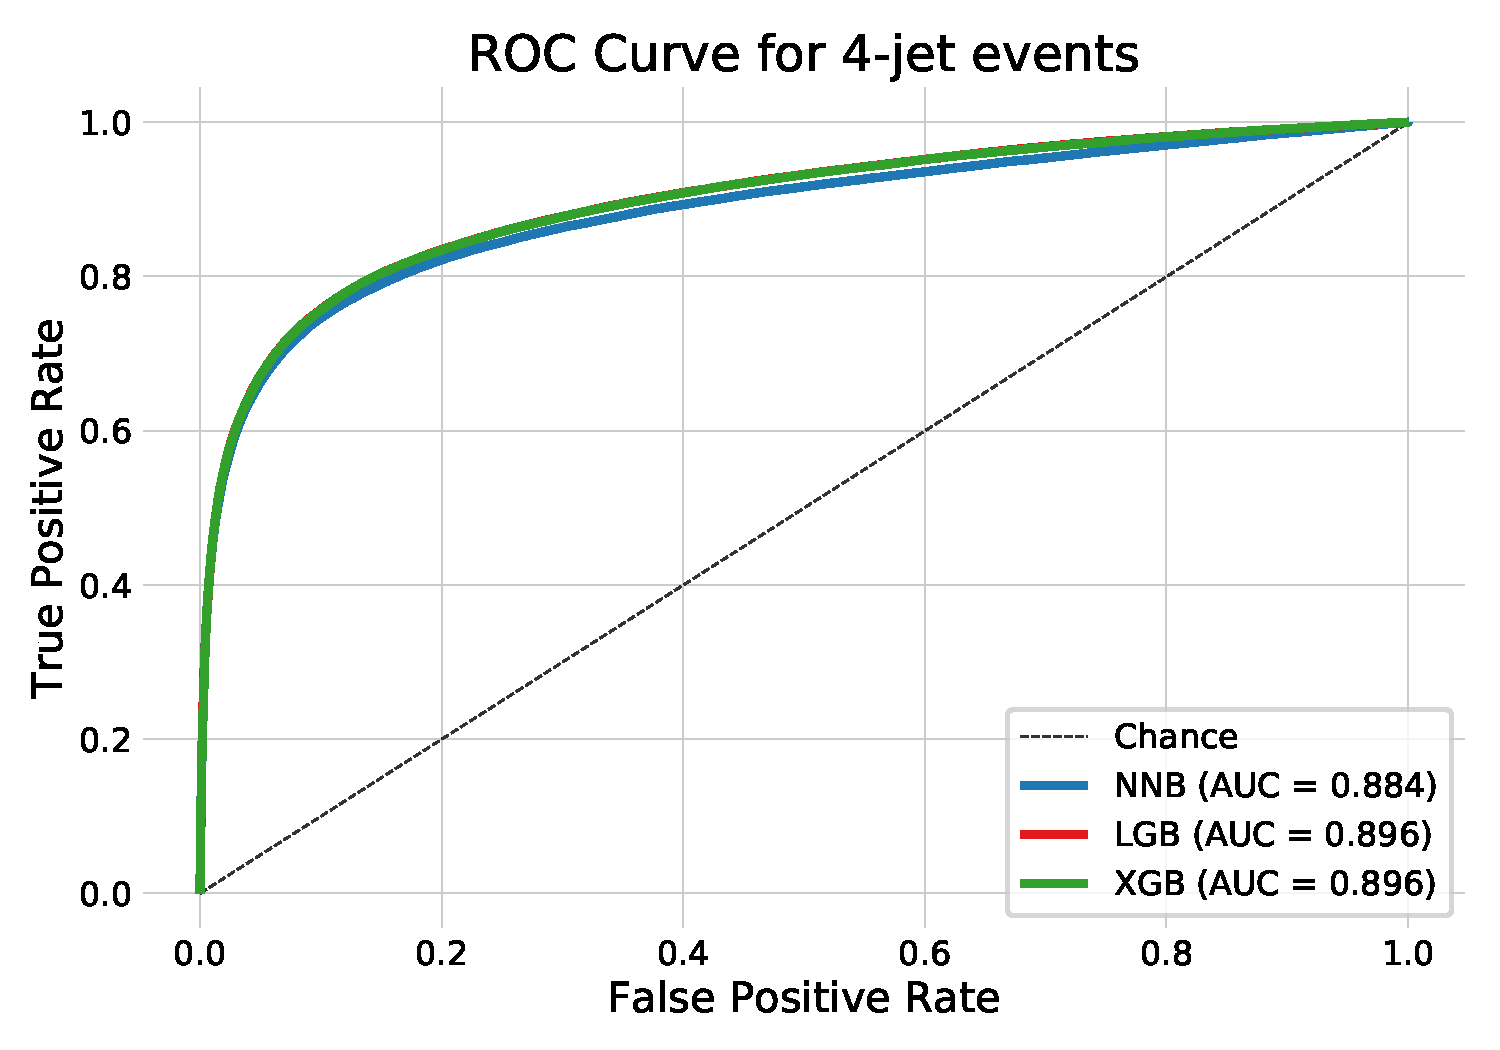
\includegraphics[width=0.95\textwidth, trim=10 10 10 40, clip]{figures/quarks/ROC_4_jet-down_sample=1.00-ML_vars=vertex-selection=b-ejet_min=4-n_iter_RS_lgb=99-n_iter_RS_xgb=9-cdot_cut=0.90-version=19.pdf}
  \caption[ROC curve for b-tag in 4-jet events][6pt]
          {ROC curve of the three b-tag models in 3-jet events for \textcolor{blue}{NNB} (the neural network trained by ATLAS, also called \code{nnbjet}) in blue, \textcolor{red}{LGB} in red, and \textcolor{green}{XGB} in green. In the legend the Area Under Curve (AUC) is also shown. Notice that the LGB and XGB models share performance and it is thus due to overplotting that only the green line for XGB can be seen. In the particle physics community False Positive Rate (FPR) is sometimes better known as background efficiency and True Positive Rate (TPR) as signal efficiency.  
          } 
  \label{fig:q:roc_btag_4j}
\end{figure}




\begin{figure}
  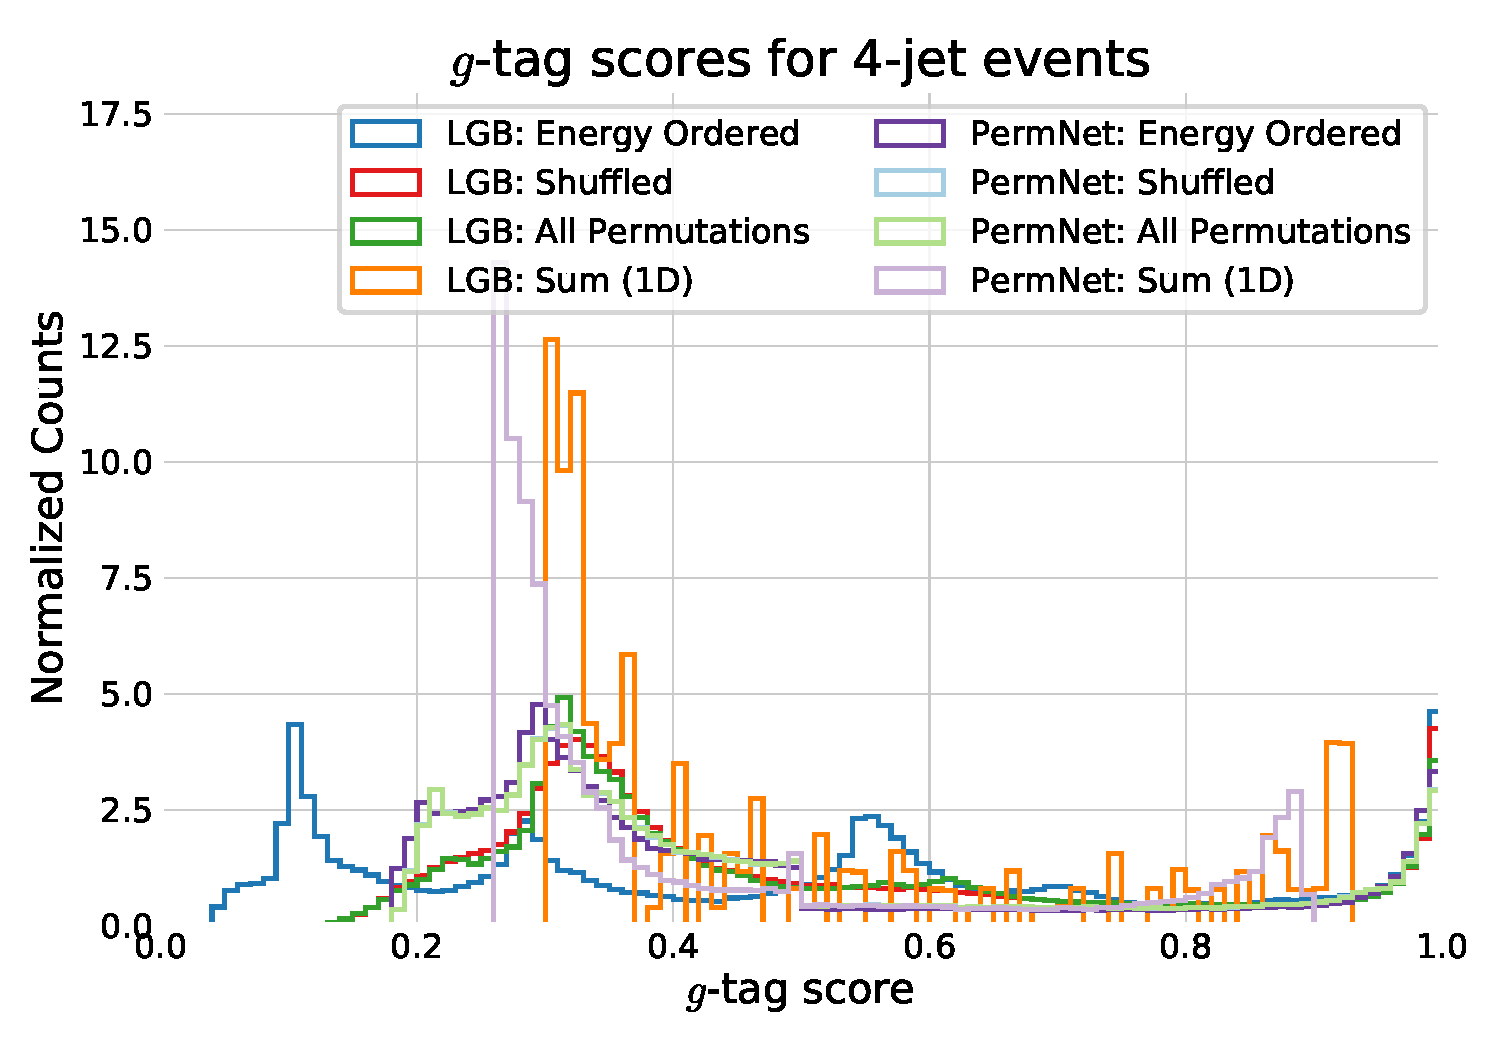
\includegraphics[width=0.95\textwidth, trim=10 10 10 40, clip]{figures/quarks/gtag_y_pred_4_jet_hist-down_sample=1.00-ML_vars=vertex-selection=b-ejet_min=4-n_iter_RS_lgb=99-n_iter_RS_xgb=9-cdot_cut=0.90-version=19.pdf}
  \caption[g-tag scores in 4-jet events][6pt]
          {
            Histogram of g-tag scores (model prediction) in 4-jet events for \textcolor{blue}{LGB: Energy Ordered} in blue, \textcolor{red}{LGB: Shuffled} in red, \textcolor{green}{LGB: All Permutations} in green, \textcolor{orange}{LGB: Sum 1D} in orange, \textcolor{purple}{PermNet: Energy Ordered} in purple, \textcolor{light-blue}{PermNet: Shuffled} in light-blue, \textcolor{light-green}{PermNet: All Permutations} in light-green, \textcolor{light-purple}{PermNet: Sum 1D} in light-purple.  Here LGB and PermNet are the two different type of models and \q{Energy Ordered}, \q{Shuffled}, \q{All Permutations}, and \q{Sum 1D} are the different methods used for making the input data permutation invariant.  
          }   
  \label{fig:q:gtag_scores_4j}
\end{figure}


\begin{figure}
  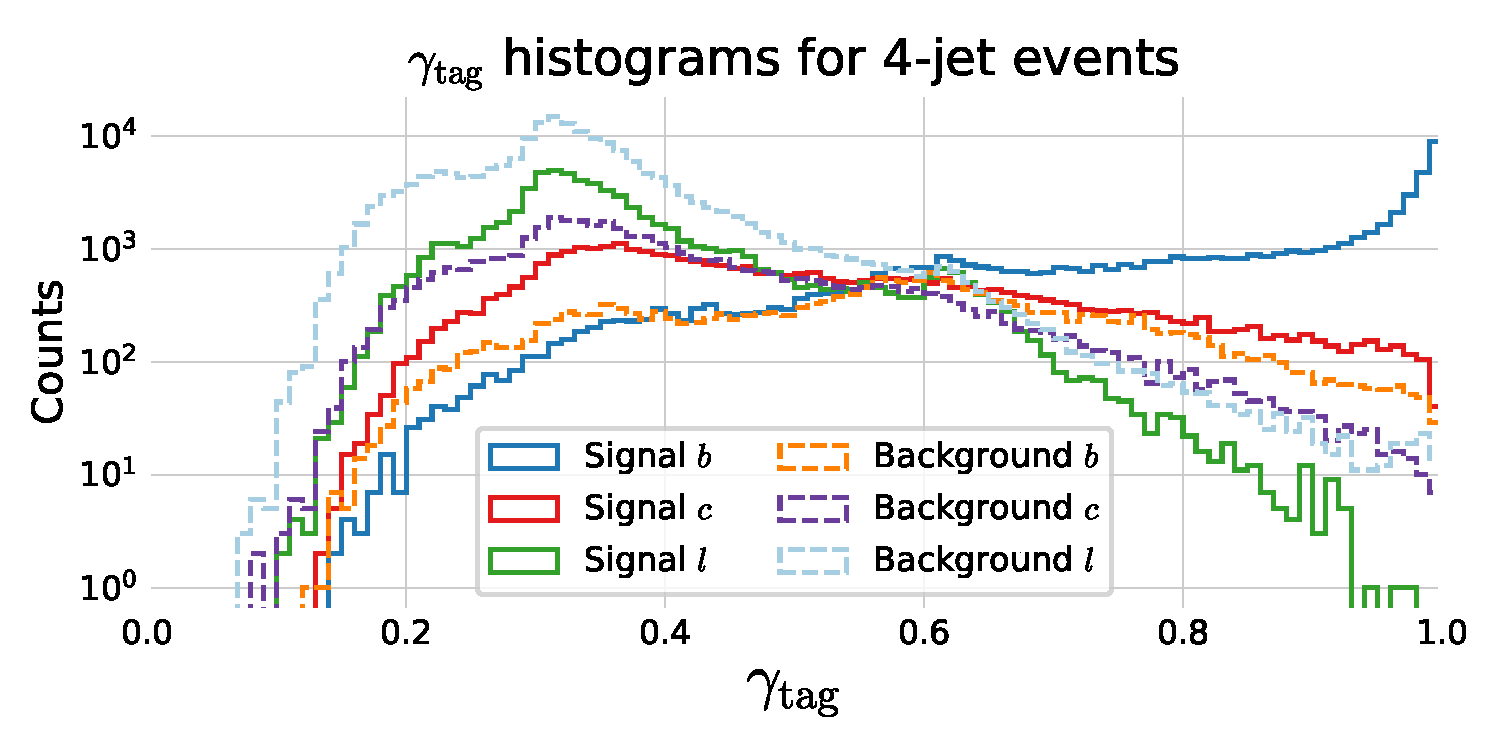
\includegraphics[width=0.95\textwidth, trim=10 10 10 40, clip]{figures/quarks/gtag-histogram-sigbkg-down_sample=1.00-ML_vars=vertex-selection=b-ejet_min=4-n_iter_RS_lgb=99-n_iter_RS_xgb=9-cdot_cut=0.90-version=19-njet=4.pdf}
  \caption[g-tag scores in 4-jet events for signal and background][6pt]
          {Histogram of g-tag scores (model prediction) from the LGB-model in 4-jet events for \textcolor{blue}{b signal} in blue, \textcolor{red}{c signal} in red, \textcolor{green}{l signal} in green, \textcolor{orange}{b background} in orange, \textcolor{purple}{c background} in purple, \textcolor{light-blue}{l background} in light-blue.
          } 
  \label{fig:q:gtag_scores_4j_sig_bkg}
\end{figure}





\begin{figure}
  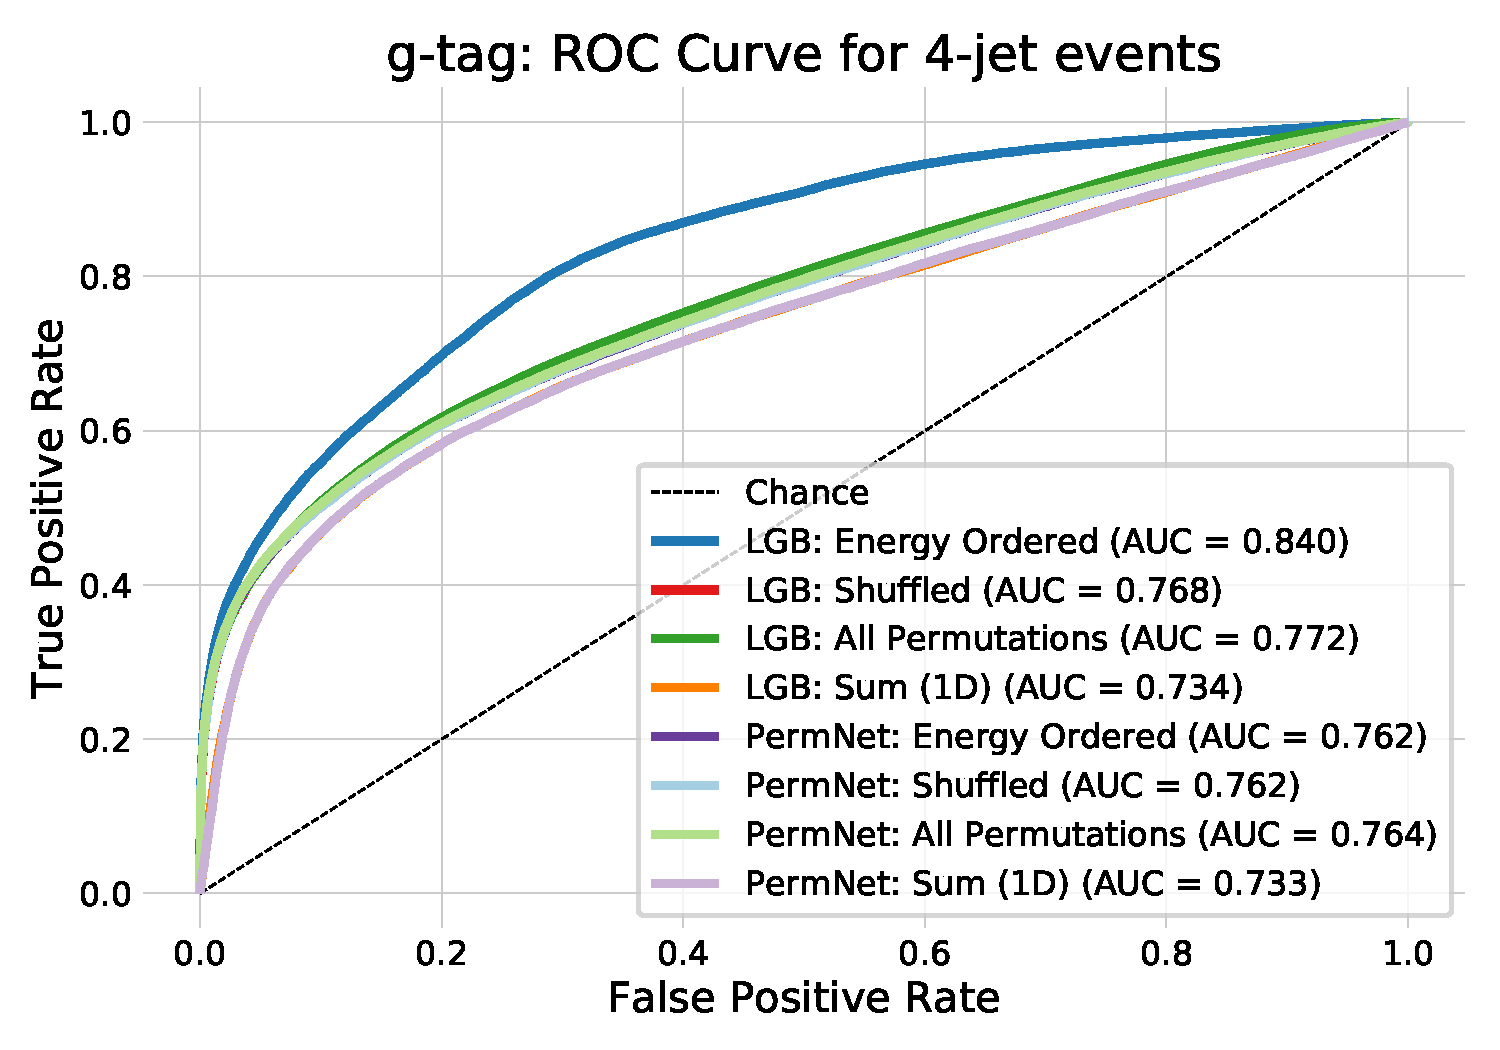
\includegraphics[width=0.95\textwidth, trim=10 10 10 40, clip]{figures/quarks/gtag_ROC_4_jet-down_sample=1.00-ML_vars=vertex-selection=b-ejet_min=4-n_iter_RS_lgb=99-n_iter_RS_xgb=9-cdot_cut=0.90-version=19.pdf}
  \caption[ROC curve for g-tag in 4-jet events][6pt]
          {ROC curve of the eight g-tag models in 4-jet events. First one in dashed black is the ROC curve that you get by random chance. The colors are the same as in \figref{fig:q:gtag_scores_4j} and in the legend also the Area Under the ROC curve (AUC) is shown. 
          Notice that the LGB model which uses the energy ordered data produced the best model, however, this model is not permutation invariant. Of the permutation invariant models (the rest), the LGB model trained on all permutations of the b-tags performs highest. The lowest performing models are the two models trained only on the 1-dimensional sum of b-tags, as expected, however, still with a better performance than expected by the author.  
          } 
  \label{fig:q:roc_gtag_4j}
\end{figure}





\begin{figure}
  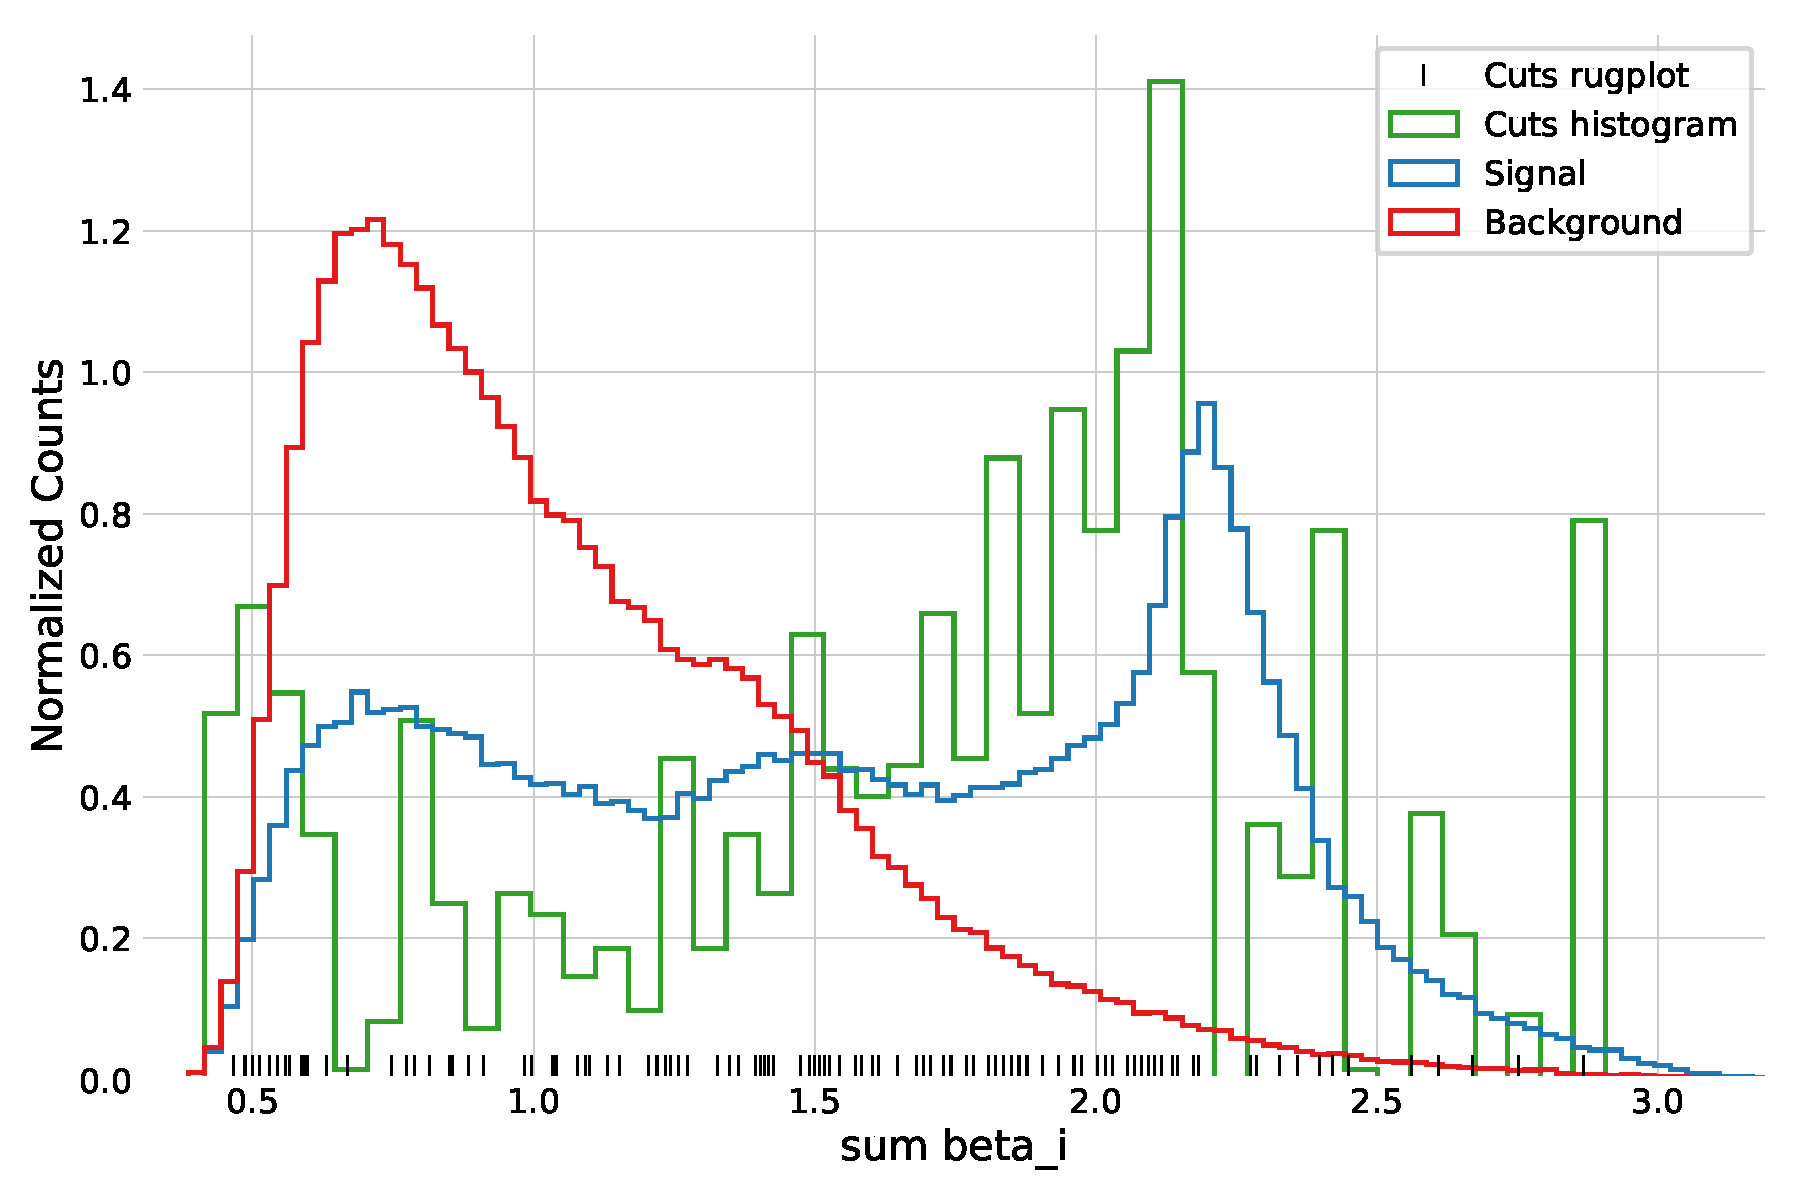
\includegraphics[width=0.95\textwidth, trim=10 10 10 20, clip]{figures/quarks/gtag_sum_method_njet=4-down_sample=1.00-ML_vars=vertex-selection=b-ejet_min=4-n_iter_RS_lgb=99-n_iter_RS_xgb=9-cdot_cut=0.90-version=19.pdf}
  \caption[1D Sum Model Cuts for 4-jets][6pt]
          {Histogram of the distribution of \textcolor{blue}{signal} in blue and \textcolor{red}{background} in red for 1-dimensional sum of b-tags training data. A histogram of the \textcolor{green}{cut values} from the LGB model trained on this data is shown in green together with a rug plot of the cut values in black. Notice how most of the cuts match up with the signal peak at around a $\sum \beta_i \sim 2.1$, however, there are also quite a lot of cuts around $\sum \beta_i \sim 0.5$.
          } 
  \label{fig:q:1d_sum_model_cuts_4j}
\end{figure}


\begin{figure}
  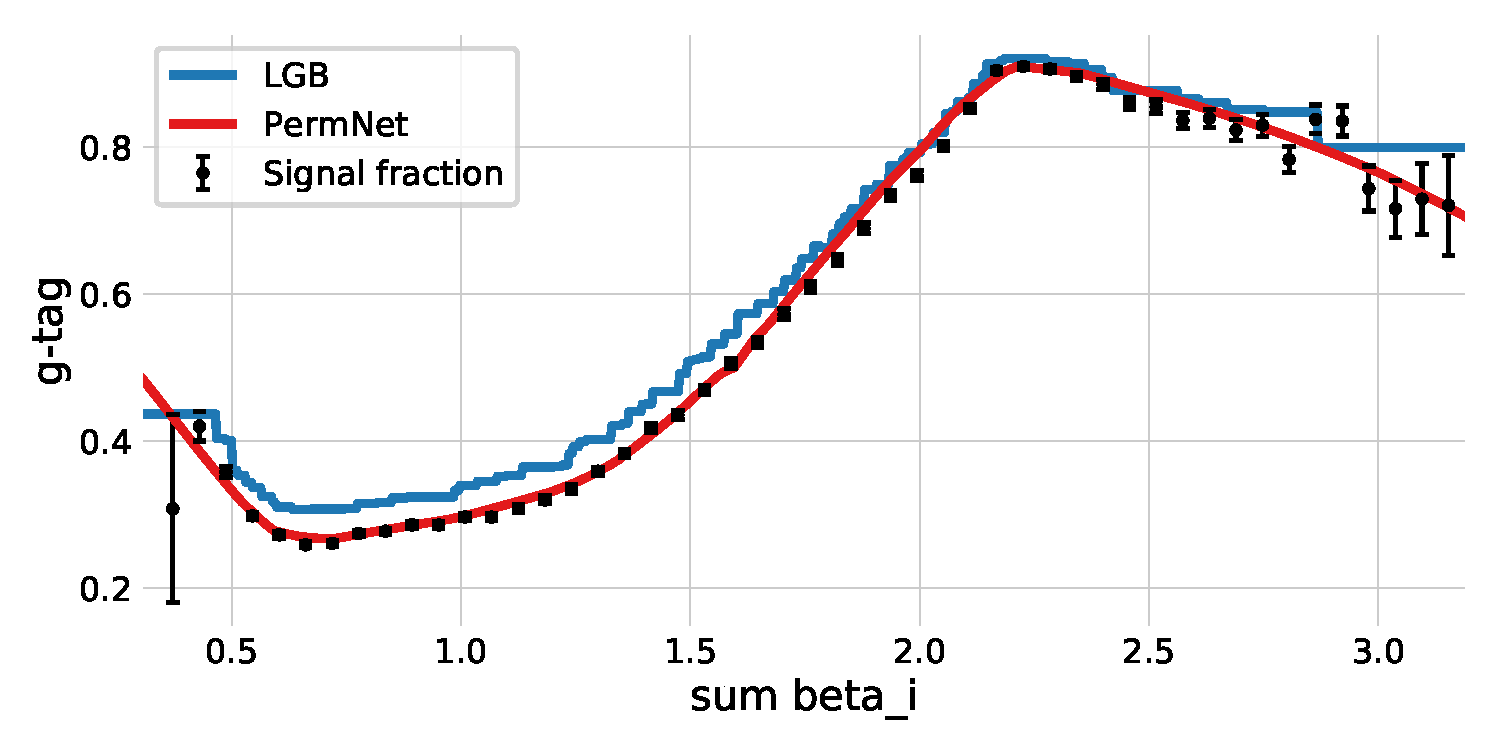
\includegraphics[width=0.95\textwidth, trim=10 10 10 20, clip]{figures/quarks/gtag_sum_models_njet=4-down_sample=1.00-ML_vars=vertex-selection=b-ejet_min=4-n_iter_RS_lgb=99-n_iter_RS_xgb=9-cdot_cut=0.90-version=19.pdf}
  \caption[1D Sum Models Predictions and Signal Fraction for 4-jets][6pt]
          {Plot of the (1D) g-tag scores as a function of $\sum \beta_i$ for the \textcolor{blue}{LGB} model in blue and the \textcolor{red}{PermNet} model in red. Here the g-tag scores are just the models' output values when input a uniformly spaced grid of $\sum \beta_i$ values between 0 and 4. The signal fraction (based on the signal and background histograms in \figref{fig:q:1d_sum_model_cuts_4j}) is plotted as black error bars where the size of the error bars is based on the propagated uncertainties of the signal and background histogram assuming Poissonian statistics. Notice how both models capture the overall trend of the signal fraction with the PermNet being particularly close. 
          } 
  \label{fig:q:1d_sum_models_signal_fraction_4j}
\end{figure}




\begin{figure}
  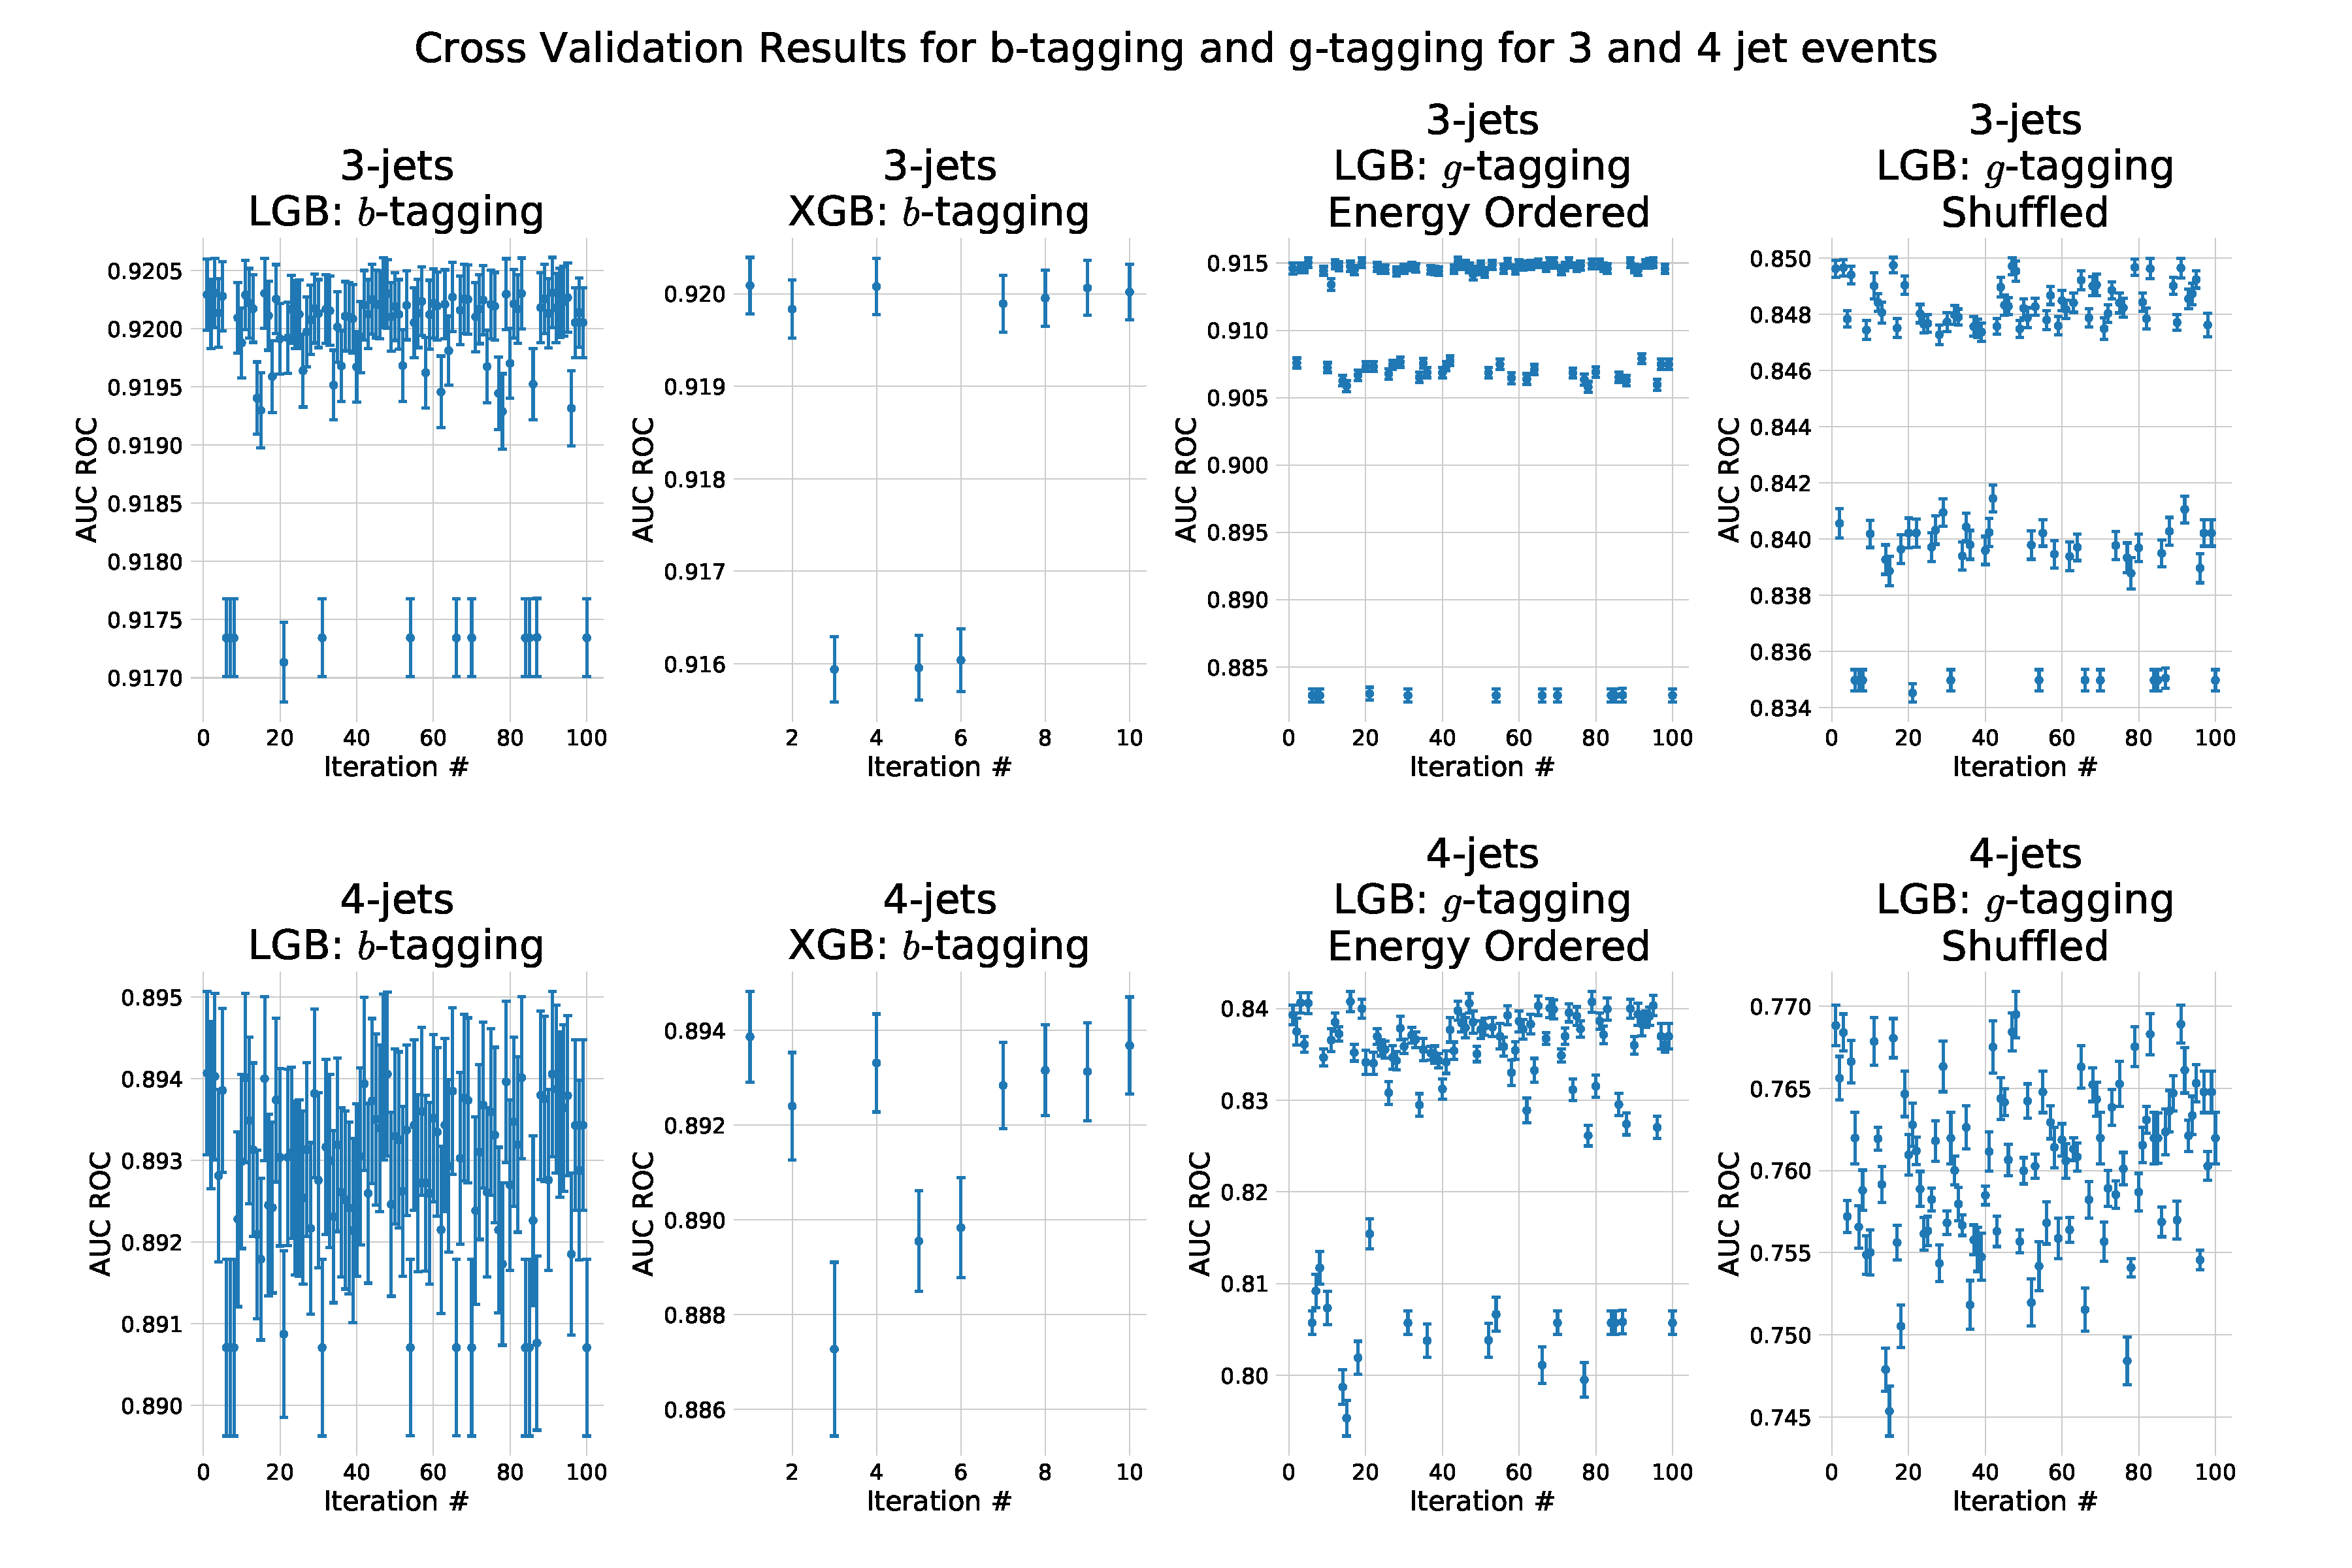
\includegraphics[width=0.95\textwidth, trim=10 10 10 60, clip]{figures/quarks/cv_res_lgb-down_sample=1.00-ML_vars=vertex-selection=b-ejet_min=4-n_iter_RS_lgb=99-n_iter_RS_xgb=9-cdot_cut=0.90-version=19.pdf}
  \caption[Hyperparameter Optimization of b- and g-tagging][6pt]
          {Hyperparameter Optimization (HPO) results after running 100 iterations of Random Search (only 10 for XGB). In the top row are the results of the 3-jet models and in the bottom row the results of the 4-jet models. From left to right, we have first) the b-tagging results of LGB, second) the b-tagging results of XGB using only 10 iterations of RS, third) the g-tagging results of LGB fit on the Energy Ordered b-tags, and forth) the g-tagging results of LGB fit on the shuffled b-tags. Notice the different ranges on the y-axes.
          } 
  \label{fig:q:CV_res_iterations}
\end{figure}


\begin{figure}
  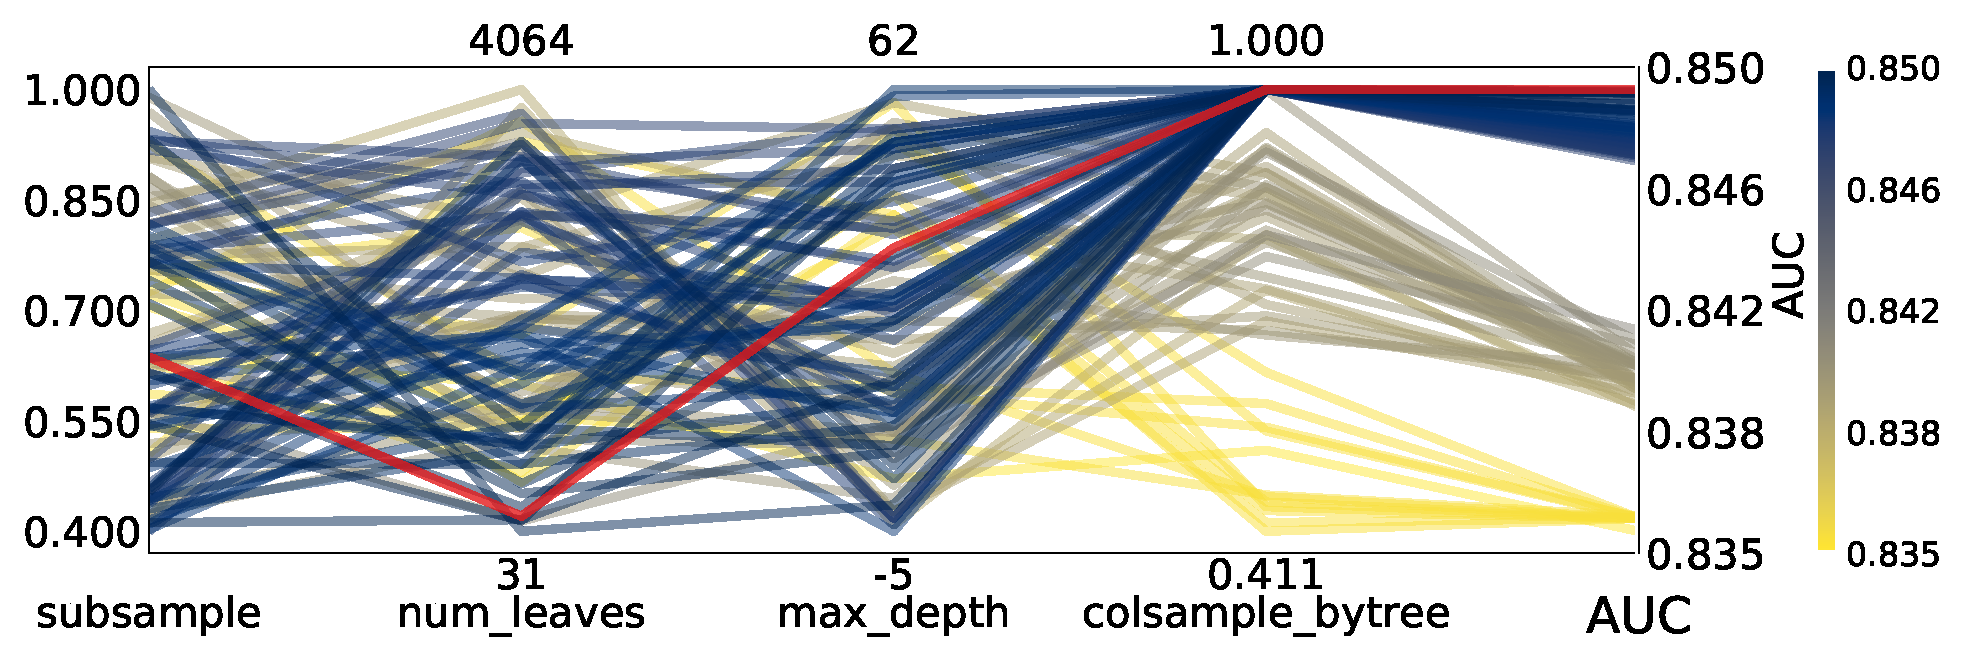
\includegraphics[width=0.95\textwidth, trim=0 0 0 0, clip]{figures/quarks/CV_viz-njet=3-name=lf_gtag_shuffled_lgb_down_sample=1.00-ML_vars=vertex-selection=b-ejet_min=4-n_iter_RS_lgb=99-n_iter_RS_xgb=9-cdot_cut=0.90-version=19.pdf}
  \caption[Overview of Hyperparamaters of g-tagging for 3-jet shuffled events][6pt]
          {Hyperparameter optimization results of g-tagging for 3-jet shuffled events. The results are shown as parallel coordinates with each hyperparameter along the x-axis and the value of that parameter on the y-axis. Each line is an event in the 4-dimensional space colored according to the performance of that hyperparameter as measured by AUC from \textcolor{viridis-dark}{highest} AUC in dark blue to \textcolor{viridis-light}{lowest} AUC in yellow. The \textcolor{red}{single best hyperparameter} is shown in red. 
          } 
  \label{fig:q:CV_res_parallel_coords}
\end{figure}



\begin{figure}
  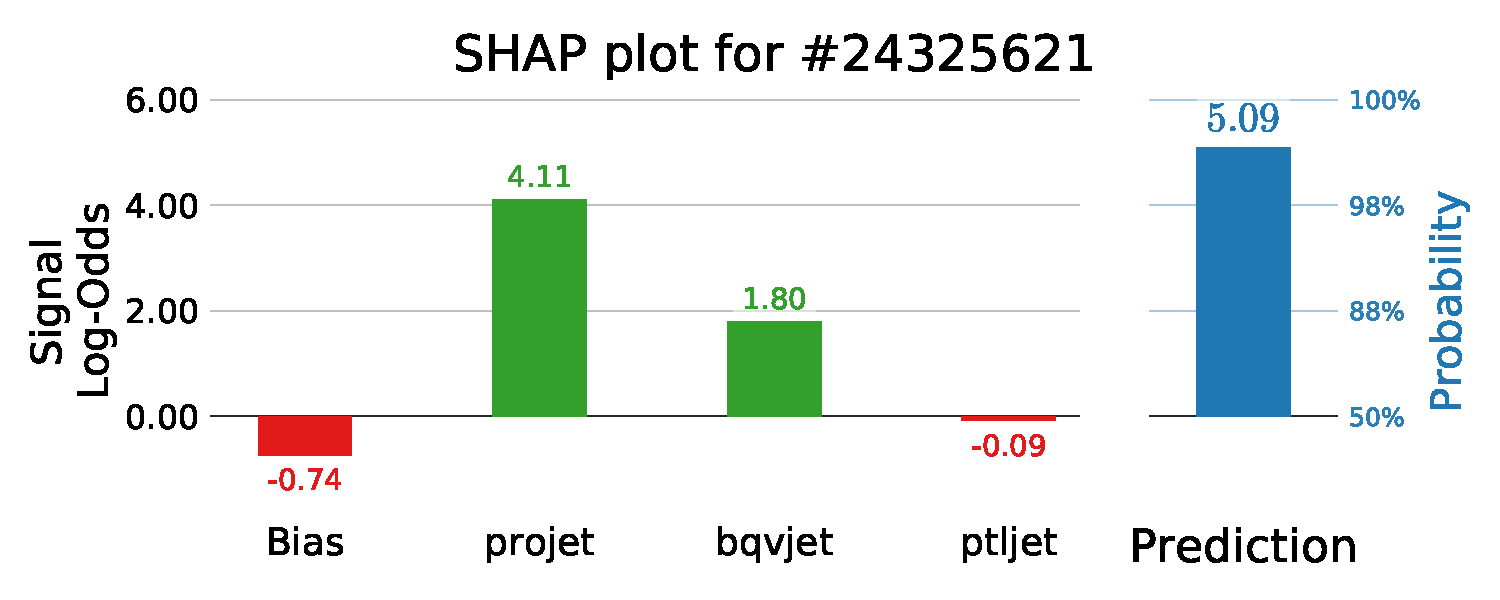
\includegraphics[width=0.95\textwidth, trim=0 0 0 40, clip]{figures/quarks/shap_values-down_sample=1.00-ML_vars=vertex-selection=b-ejet_min=4-n_iter_RS_lgb=99-n_iter_RS_xgb=9-cdot_cut=0.90-version=19-njet=3loc=24325621.pdf}
  \caption[SHAP Prediction Explanation for b-like jet][6pt]
          {Model explanation for the 3-jet b-tagging model for a b-like jet. The first column is the bias of the training set which acts as the naive prediction baseline, the rest are the input data variables. On the right hand side of the plot is the model prediction shown. The left part of the plot is shown in log-odds space, the right part in probability space. The model prediction is the sum of the log-odds (5.09 in this example) transformed into probability space. The \textcolor{red}{negative} log-odd values are shown in red, \textcolor{green}{positive} ones in green, and the \textcolor{blue}{prediction value} in blue. 
          } 
  \label{fig:q:shap_signal}
\end{figure}


\begin{figure}
  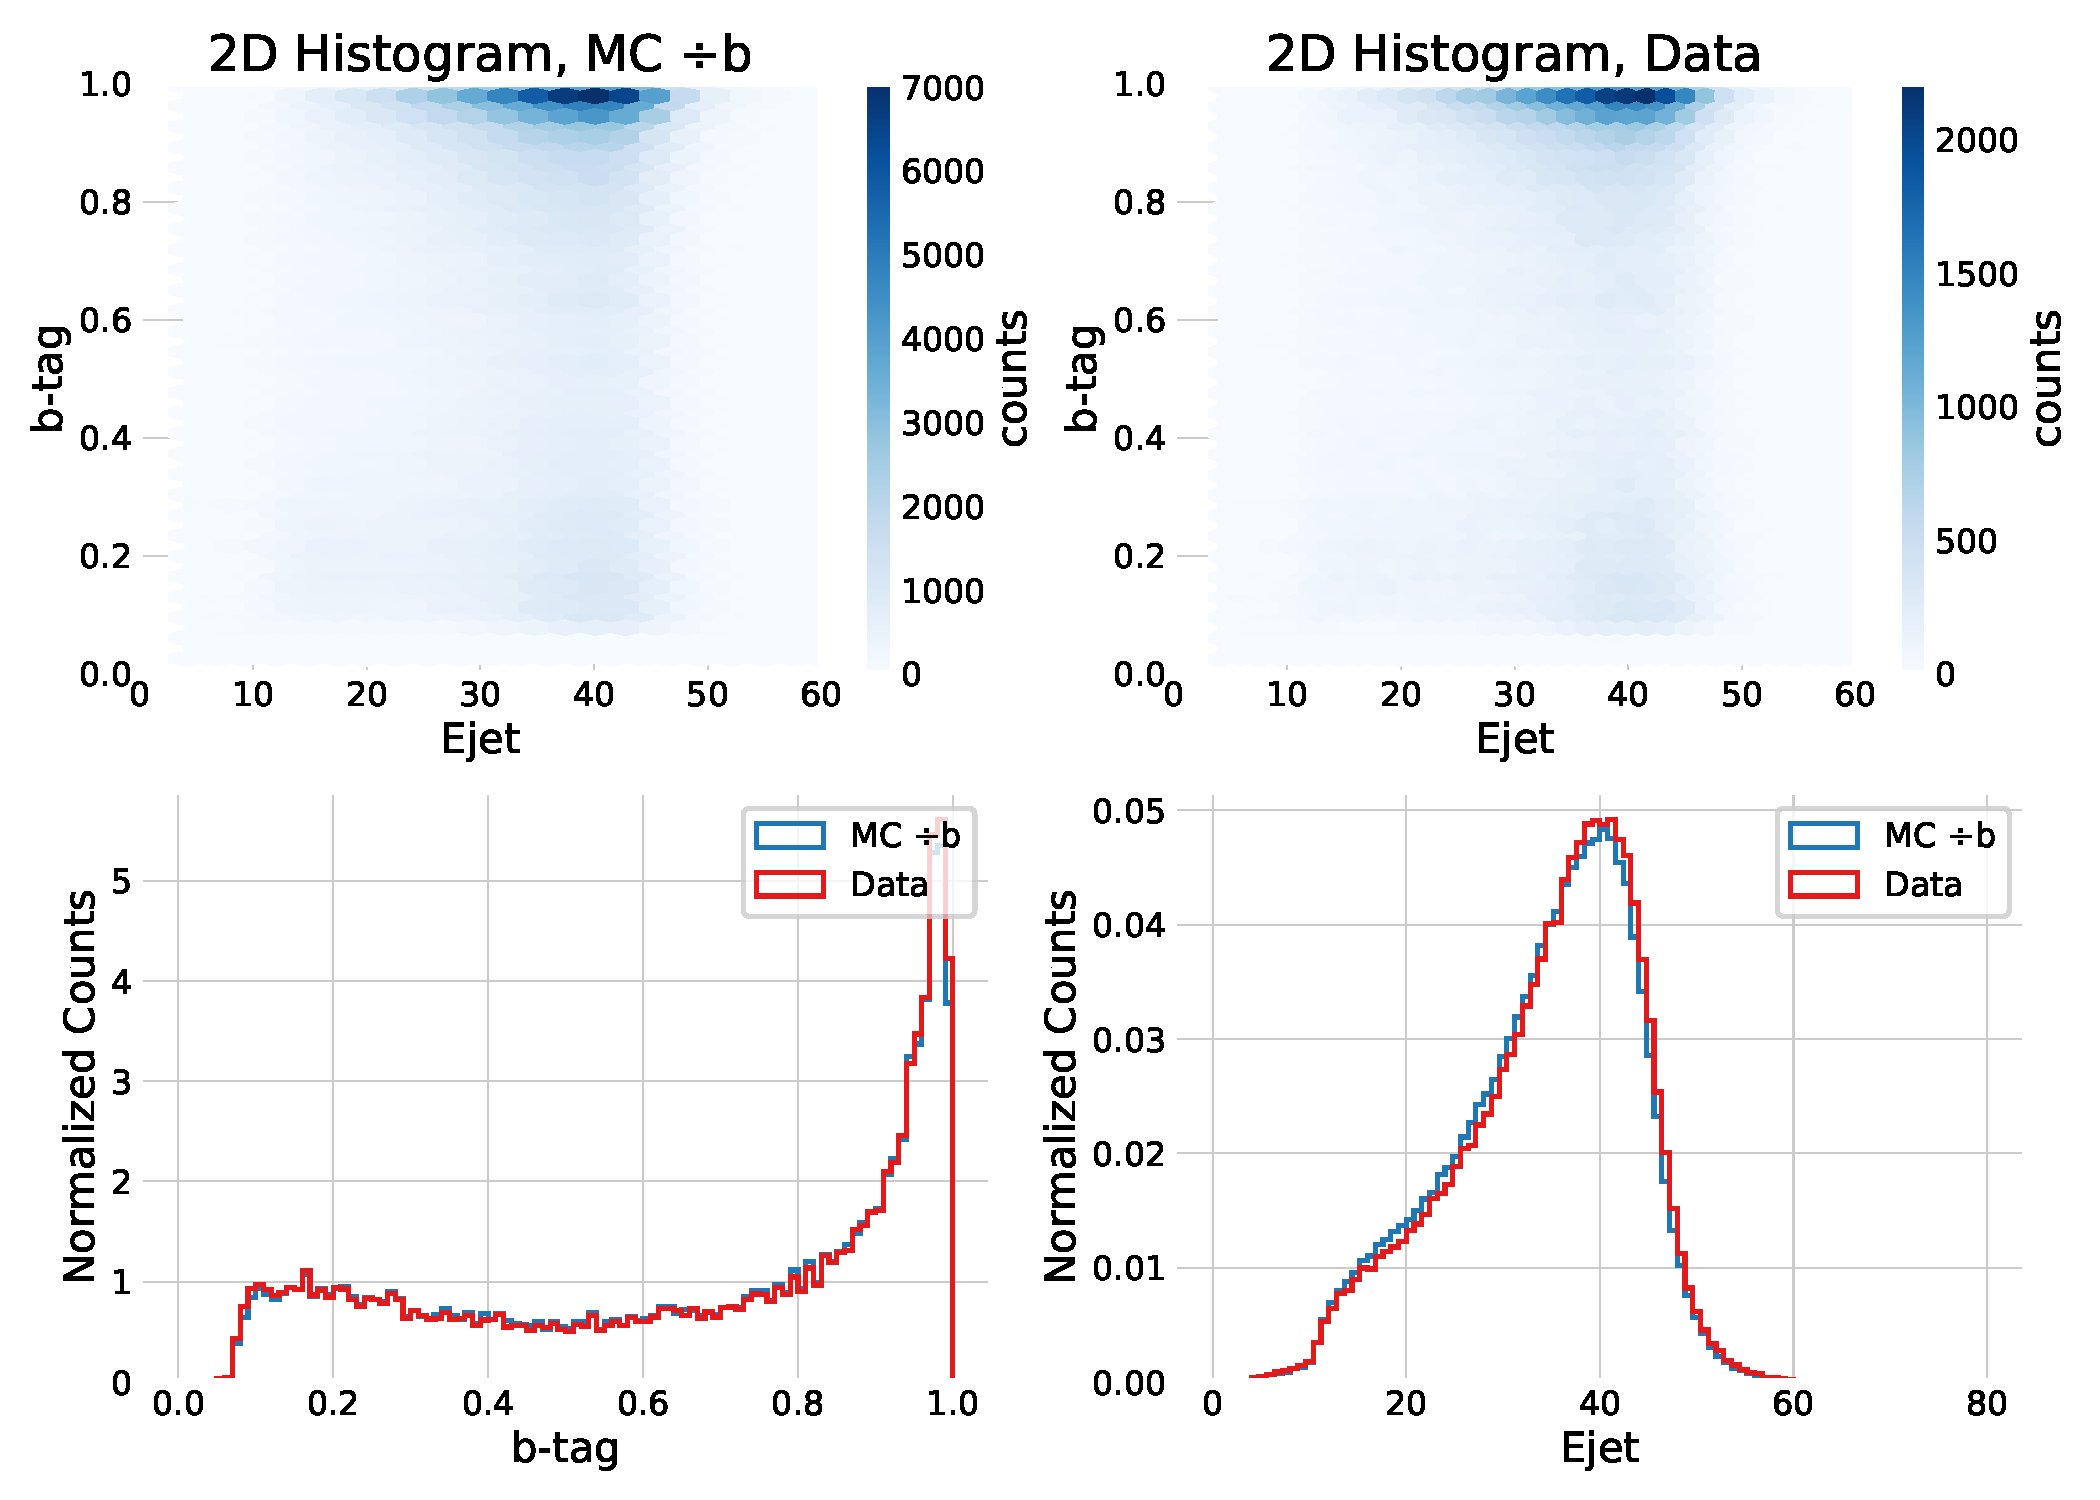
\includegraphics[width=0.95\textwidth, trim=0 0 0 40, clip]{figures/quarks/2d-histograms-ejet-btag-comparison-down_sample=1.00-ML_vars=vertex-selection=b-ejet_min=4-n_iter_RS_lgb=99-n_iter_RS_xgb=9-cdot_cut=0.90-version=19-njet=3.pdf}
  \caption[Monte Carlo -- Data bias for b-tags and jet energy][6pt]
          {Comparison of the b-tag and jet energy (\code{Ejet}) distributions for Monte Carlo (MC) versus data. In the top row the 2D-distributions are shown for MC on the left (without the extra MCb samples) and data on the right. In the bottom row the 1D marginal distrubtions are shown for the b-tag and the jet energy with \textcolor{red}{data} in red and \textcolor{blue}{Monte Carlo} ones in blue. Notice the the almost identical distributions in b-tag. 
          } 
  \label{fig:q:btag_Ejet_comparison}
\end{figure}

\begin{figure}
  \includegraphics[width=0.95\textwidth, trim=0 0 0 40, clip]{figures/quarks/eff_b_bsig-down_sample=1.00-ML_vars=vertex-selection=b-ejet_min=4-n_iter_RS_lgb=99-n_iter_RS_xgb=9-cdot_cut=0.90-version=19.pdf}
  \caption[b-Tagging Efficiency $\varepsilon_b^{b\mathrm{-sig}}$ as a function of jet energy][6pt]
          {Efficiency of the b-tags for b-jets in the b-signal region for 3-jet events, $\varepsilon_b^{b\mathrm{-sig}}$, as a function of jet energy \code{Ejet}. The b-signal region is defined as $\beta > 0.9$. In the plot the efficiencies are shown for \textcolor{blue}{MC Truth} in blue, \textcolor{red}{MC TTP} in red, \textcolor{green}{MC Truth TTP} in green, and \textcolor{orange}{Data TTP} in orange. The efficiencies (the errorbars) can be read off on the left y-axis and the counts (histograms) on the right y-axis. The abbreviation TTP is short for \q{Tag, Tag, Probe} where two jets in a event are used as tags and the probe is then used for further analysis. Notice how both MC TTP and Data TTP follow each other closely.  
          } 
  \label{fig:q:effiency_btag_bjet_bsig}
\end{figure}


\begin{figure}
  \includegraphics[width=0.95\textwidth, trim=0 0 0 40, clip]{figures/quarks/eff_b_gsig-down_sample=1.00-ML_vars=vertex-selection=b-ejet_min=4-n_iter_RS_lgb=99-n_iter_RS_xgb=9-cdot_cut=0.90-version=19.pdf}
  \caption[b-Tagging Efficiency $\varepsilon_b^{g\mathrm{-sig}}$ as a function of jet energy][6pt]
          {Efficiency of the b-tags for b-jets in the g-signal region for 3-jet events, $\varepsilon_b^{g\mathrm{-sig}}$, as a function of jet energy \code{Ejet}. The g-signal region is defined as $\beta < 0.4$. In the plot the efficiencies are shown for \textcolor{blue}{MC Truth} in blue, \textcolor{red}{MC TTP} in red, \textcolor{green}{MC Truth TTP} in green, and \textcolor{orange}{Data TTP} in orange. The efficiencies (the errorbars) can be read off on the left y-axis and the counts (histograms) on the right y-axis. The abbreviation TTP is short for \q{Tag, Tag, Probe} where two jets in a event are used as tags and the probe is then used for further analysis. Notice how both MC TTP and Data TTP follow each other closely.  
          } 
  \label{fig:q:effiency_btag_bjet_gsig}
\end{figure}


\begin{figure}
  \includegraphics[width=0.95\textwidth, trim=0 0 0 40, clip]{figures/quarks/eff_g_gsig-down_sample=1.00-ML_vars=vertex-selection=b-ejet_min=4-n_iter_RS_lgb=99-n_iter_RS_xgb=9-cdot_cut=0.90-version=19.pdf}
  \caption[b-Tagging Efficiency $\varepsilon_g^{g\mathrm{-sig}}$ as a function of jet energy][6pt]
          {Efficiency of the b-tags for g-jets in the g-signal region for 3-jet events, $\varepsilon_g^{g\mathrm{-sig}}$, as a function of jet energy \code{Ejet}. The g-signal region is defined as $\beta < 0.4$. In the plot the efficiencies are shown for \textcolor{blue}{MC Truth} in blue, \textcolor{red}{MC TTP} in red, \textcolor{green}{MC Truth TTP} in green, and \textcolor{orange}{Data TTP} in orange. The efficiencies (the errorbars) can be read off on the left y-axis and the counts (histograms) on the right y-axis. The abbreviation TTP is short for \q{Tag, Tag, Probe} where two jets in a event are used as tags and the probe is then used for further analysis. Notice how both MC TTP and Data TTP follow each other closely.  
          } 
  \label{fig:q:effiency_btag_gjet_gsig}
\end{figure}

\begin{figure}
  \includegraphics[width=0.95\textwidth, trim=0 0 0 30, clip]{figures/quarks/eff_g_bsig-down_sample=1.00-ML_vars=vertex-selection=b-ejet_min=4-n_iter_RS_lgb=99-n_iter_RS_xgb=9-cdot_cut=0.90-version=19.pdf}
  \caption[b-Tagging Efficiency $\varepsilon_g^{b\mathrm{-sig}}$ as a function of jet energy][6pt]
          {Efficiency of the b-tags for g-jets in the b-signal region for 3-jet events, $\varepsilon_g^{b\mathrm{-sig}}$, as a function of jet energy \code{Ejet}. The b-signal region is defined as $\beta > 0.9$. In the plot the efficiencies are shown for \textcolor{blue}{MC Truth} in blue, \textcolor{red}{MC TTP} in red, \textcolor{green}{MC Truth TTP} in green, and \textcolor{orange}{Data TTP} in orange. The efficiencies (the errorbars) can be read off on the left y-axis and the counts (histograms) on the right y-axis. The abbreviation TTP is short for \q{Tag, Tag, Probe} where two jets in a event are used as tags and the probe is then used for further analysis.  
          } 
  \label{fig:q:effiency_btag_gjet_bsig}
\end{figure}


\begin{figure}
  \includegraphics[width=0.95\textwidth, trim=0 0 0 40, clip]{figures/quarks/eff_bbg_m_mean-down_sample=1.00-ML_vars=vertex-selection=b-ejet_min=4-n_iter_RS_lgb=99-n_iter_RS_xgb=9-cdot_cut=0.90-version=19.pdf}
  \caption[g-Tagging proxy efficiency for $b\bar{b}g$-events as function of the mean invariant mass][6pt]
          {Proxy efficiency of the g-tags for $b\bar{b}g$ 3-jet events as a function of the mean of the two invariant masses $m_{bg}$ and $m_{\bar{b}g}$. The proxy efficiency $\varepsilon_{b\bar{b}g}$ is measured by finding $b\bar{b}g$-events where $\beta_b > 0.9$, $\beta_{\bar{b}}>0.9$, and $\beta_g < 0.4$. and then calculating  $\varepsilon_{b\bar{b}g} = \varepsilon_b^{b\mathrm{-sig}} \cdot \varepsilon_{\bar{b}}^{b\mathrm{-sig}} \cdot  \varepsilon_g^{g\mathrm{-sig}} $. In the top plot $\varepsilon_{b\bar{b}g}$ is shown for \textcolor{blue}{MC} in blue and \textcolor{red}{Data} in red where the counts in each bin can be read on right y-axis. In the bottom plot the ratio between Data and MC is shown.
          } 
  \label{fig:q:effiency_btag_bbg_m_mean}
\end{figure}


\begin{figure}
  \includegraphics[width=0.95\textwidth, trim=0 0 0 40, clip]{figures/quarks/eff_bbg_gtag-down_sample=1.00-ML_vars=vertex-selection=b-ejet_min=4-n_iter_RS_lgb=99-n_iter_RS_xgb=9-cdot_cut=0.90-version=19.pdf}
  \caption[g-Tagging proxy efficiency for $b\bar{b}g$-events as function of g-tag][6pt]
          {Proxy efficiency of the g-tags for $b\bar{b}g$ 3-jet events as a function of the event's g-tag. The proxy efficiency $\varepsilon_{b\bar{b}g}$ is measured by finding $b\bar{b}g$-events where $\beta_b > 0.9$, $\beta_{\bar{b}}>0.9$, and $\beta_g < 0.4$. and then calculating  $\varepsilon_{b\bar{b}g} = \varepsilon_b^{b\mathrm{-sig}} \cdot \varepsilon_{\bar{b}}^{b\mathrm{-sig}} \cdot  \varepsilon_g^{g\mathrm{-sig}} $. In the top plot $\varepsilon_{b\bar{b}g}$ is shown for \textcolor{blue}{MC} in blue and \textcolor{red}{Data} in red where the counts in each bin can be read on right y-axis. In the bottom plot the ratio between Data and MC is shown.
          } 
  \label{fig:q:effiency_btag_bbg_gtag}
\end{figure}



\begin{figure}
  \includegraphics[width=0.95\textwidth, trim=0 0 0 40, clip, page=1]{figures/quarks/efficiency_events-down_sample=1.00-ML_vars=vertex-selection=b-ejet_min=4-n_iter_RS_lgb=99-n_iter_RS_xgb=9-cdot_cut=0.90-version=19-njet=4.pdf}
  \caption[g-Tagging efficiency for 4-jet events in MC as a function of normalized gluon gluon jet energy difference][6pt]
          {Efficiency of the g-tags for 4-jet events as a function of normalized gluon gluon jet energy difference in Monte Carlo. The efficiency is measured as the number of events with a g-tag higher than 0.8 ($\gamma > 0.8$) out of the total number and the normalized gluon gluon jet energy difference $A$ is $A=\frac{E_{g_\mathrm{max}}-E_{g_\mathrm{min}}}{E_{g_\mathrm{max}}+E_{g_\mathrm{min}}}$ where $E_{g_\mathrm{max}}$ ($E_{g_\mathrm{min}}$) refers to the energy of the gluon with the highest (lowest) energy. The efficiency is plotted for \textcolor{blue}{signal events} according to MC Truth in blue and \textcolor{red}{background events} according to MC Truth in red.
          } 
  \label{fig:q:effiency_gtag_E_diff}
\end{figure}


\begin{figure}
  \includegraphics[width=0.95\textwidth, trim=0 0 0 65, clip, page=1]{figures/quarks/gtag-closure_test-down_sample=1.00-ML_vars=vertex-selection=b-ejet_min=4-n_iter_RS_lgb=99-n_iter_RS_xgb=9-cdot_cut=0.90-version=19-njet=3.pdf}
  \caption[Closure plot between MC Truth and the corrected g-tagging model in 4-jet events for the normalized gluon gluon jet energy difference][6pt]
          {Closure plot between MC Truth and the corrected g-tagging model in 4-jet events for the normalized gluon gluon jet energy difference. The corrected g-taggingg model is described in further detail in section XXX \TODO. In the top part of the plot the \textcolor{blue}{MC Truth} is shown in blue, the \textcolor{red}{corrected g-tagging model} \code{"PDF 2gg"} in red, the \textcolor{green}{g-signal distribution} in semi-transparent green and the \textcolor{orange}{g-sideband distribution} in semi-transparent orange. In the bottom part of the plot the ratio between MC Truth and the output of the corrected g-tagging model is shown. The normalized gluon gluon jet energy difference $A$ is $A=\frac{E_{g_\mathrm{max}}-E_{g_\mathrm{min}}}{E_{g_\mathrm{max}}+E_{g_\mathrm{min}}}$ where $E_{g_\mathrm{max}}$ ($E_{g_\mathrm{min}}$) refers to the energy of the gluon with the highest (lowest) energy.
          } 
  \label{fig:q:closure_E_diff}
\end{figure}


\begin{figure}
  \includegraphics[width=0.95\textwidth, trim=0 0 0 118, clip, page=1]{figures/quarks/gtag-R_kt_CA_overview-down_sample=1.00-ML_vars=vertex-selection=b-ejet_min=4-n_iter_RS_lgb=99-n_iter_RS_xgb=9-cdot_cut=0.90-version=19-njet=4}
  \caption[R kt CA overview  XXX \TODO][6pt]
          {R kt CA overview XXX \TODO
          } 
  \label{fig:q:R_kt_CA_overview}
\end{figure}

\begin{figure}
  \includegraphics[width=0.95\textwidth, trim=0 0 0 30, clip, page=2]{figures/quarks/gtag-R_kt_CA_overview-down_sample=1.00-ML_vars=vertex-selection=b-ejet_min=4-n_iter_RS_lgb=99-n_iter_RS_xgb=9-cdot_cut=0.90-version=19-njet=4}
  \caption[R kt CA cut region A  XXX \TODO][6pt]
          {R kt CA cut region A XXX \TODO
          } 
  \label{fig:q:R_kt_CA_cut_A}
\end{figure}


The specification of the \doccmddef{sidenote} command is:
\begin{docspec}
  \doccmd{sidenote}[\docopt{number}][\docopt{offset}]\{\docarg{Sidenote text.}\}
\end{docspec}

Both the \docopt{number} and \docopt{offset} arguments are optional.  If you
provide a \docopt{number} argument, then that number will be used as the
sidenote number.  It will change of the number of the current sidenote only and
will not affect the numbering sequence of subsequent sidenotes.

Sometimes a sidenote may run over the top of other text or graphics in the
margin space.  If this happens, you can adjust the vertical position of the
sidenote by providing a dimension in the \docopt{offset} argument.  Some
examples of valid dimensions are:
\begin{docspec}
  \ttfamily 1.0in \qquad 2.54cm \qquad 254mm \qquad 6\Verb|\baselineskip|
\end{docspec}
If the dimension is positive it will push the sidenote down the page; if the
dimension is negative, it will move the sidenote up the page.

While both the \docopt{number} and \docopt{offset} arguments are optional, they
must be provided in order.  To adjust the vertical position of the sidenote
while leaving the sidenote number alone, use the following syntax:
\begin{docspec}
  \doccmd{sidenote}[][\docopt{offset}]\{\docarg{Sidenote text.}\}
\end{docspec}
The empty brackets tell the \Verb|\sidenote| command to use the default
sidenote number.

If you \emph{only} want to change the sidenote number, however, you may
completely omit the \docopt{offset} argument:
\begin{docspec}
  \doccmd{sidenote}[\docopt{number}]\{\docarg{Sidenote text.}\}
\end{docspec}

The \doccmddef{marginnote} command has a similar \docarg{offset} argument:
\begin{docspec}
  \doccmd{marginnote}[\docopt{offset}]\{\docarg{Margin note text.}\}
\end{docspec}

\section{References}
References are placed alongside their citations as sidenotes,
as well.  This can be accomplished using the normal \doccmddef{citep}
command.\sidenote{The first paragraph of this document includes a citation.}

The complete list of references may also be printed automatically by using
the \doccmddef{bibliography} command.  (See the end of this document for an
example.)  If you do not want to print a bibliography at the end of your
document, use the \doccmddef{nobibliography} command in its place.  


\section{Figures and Tables}\label{sec:figures-and-tables}
Images and graphics play an integral role in Tufte's work.
In addition to the standard \docenvdef{figure} and \docenvdef{tabular} environments,
this style provides special figure and table environments for full-width
floats.

Full page--width figures and tables may be placed in \docenvdef{figure*} or
\docenvdef{table*} environments.  To place figures or tables in the margin,
use the \docenvdef{marginfigure} or \docenvdef{margintable} environments as follows
(see figure~\ref{fig:marginfig}):

\begin{marginfigure}%
  \includegraphics[width=\linewidth]{helix}
  \caption{This is a margin figure.  The helix is defined by 
    $x = \cos(2\pi z)$, $y = \sin(2\pi z)$, and $z = [0, 2.7]$.  The figure was
    drawn using Asymptote (\url{http://asymptote.sf.net/}).}
  \label{fig:marginfig}
\end{marginfigure}

\begin{docspec}
\textbackslash begin\{marginfigure\}\\
  \qquad\textbackslash includegraphics\{helix\}\\
  \qquad\textbackslash caption\{This is a margin figure.\}\\
  \qquad\textbackslash label\{fig:marginfig\}\\
\textbackslash end\{marginfigure\}\\
\end{docspec}

The \docenv{marginfigure} and \docenv{margintable} environments accept an optional parameter \docopt{offset} that adjusts the vertical position of the figure or table.  See the ``\nameref{sec:sidenotes}'' section above for examples.  The specifications are:
\begin{docspec}
  \textbackslash{begin\{marginfigure\}[\docopt{offset}]}\\
  \qquad\ldots\\
  \textbackslash{end\{marginfigure\}}\\
  \mbox{}\\
  \textbackslash{begin\{margintable\}[\docopt{offset}]}\\
  \qquad\ldots\\
  \textbackslash{end\{margintable\}}\\
\end{docspec}

Figure~\ref{fig:fullfig} is an example of the \docenv{figure*}
environment and figure~\ref{fig:textfig} is an example of the normal
\docenv{figure} environment.

\begin{figure*}[h]
  \includegraphics[width=\linewidth]{sine.pdf}%
  \caption{This graph shows $y = \sin x$ from about $x = [-10, 10]$.
  \emph{Notice that this figure takes up the full page width.}}%
  \label{fig:fullfig}%
\end{figure*}

\begin{figure}
  \includegraphics{hilbertcurves.pdf}
%  \checkparity This is an \pageparity\ page.%
  \caption[Hilbert curves of various degrees $n$.][6pt]{Hilbert curves of various degrees $n$. \emph{Notice that this figure only takes up the main textblock width.}}
  \label{fig:textfig}
  %\zsavepos{pos:textfig}
\end{figure}

As with sidenotes and marginnotes, a caption may sometimes require vertical
adjustment. The \doccmddef{caption} command now takes a second optional
argument that enables you to do this by providing a dimension \docopt{offset}.
You may specify the caption in any one of the following forms:
\begin{docspec}
  \doccmd{caption}\{\docarg{long caption}\}\\
  \doccmd{caption}[\docarg{short caption}]\{\docarg{long caption}\}\\
  \doccmd{caption}[][\docopt{offset}]\{\docarg{long caption}\}\\
  \doccmd{caption}[\docarg{short caption}][\docopt{offset}]%
                  \{\docarg{long caption}\}
\end{docspec}
A positive \docopt{offset} will push the caption down the page. The short
caption, if provided, is what appears in the list of figures/tables, otherwise
the ``long'' caption appears there. Note that although the arguments
\docopt{short caption} and \docopt{offset} are both optional, they must be
provided in order. Thus, to specify an \docopt{offset} without specifying a
\docopt{short caption}, you must include the first set of empty brackets
\Verb|[]|, which tell \doccmd{caption} to use the default ``long'' caption. As
an example, the caption to figure~\ref{fig:textfig} above was given in the form
\begin{docspec}
  \doccmd{caption}[Hilbert curves...][6pt]\{Hilbert curves...\}
\end{docspec}

Table~\ref{tab:normaltab} shows table created with the \docpkg{booktabs}
package.  Notice the lack of vertical rules---they serve only to clutter
the table's data.

\begin{table}[ht]
  \centering
  \fontfamily{ppl}\selectfont
  \begin{tabular}{ll}
    \toprule
    Margin & Length \\
    \midrule
    Paper width & \unit[8\nicefrac{1}{2}]{inches} \\
    Paper height & \unit[11]{inches} \\
    Textblock width & \unit[6\nicefrac{1}{2}]{inches} \\
    Textblock/sidenote gutter & \unit[\nicefrac{3}{8}]{inches} \\
    Sidenote width & \unit[2]{inches} \\
    \bottomrule
  \end{tabular}
  \caption{Here are the dimensions of the various margins used in the Tufte-handout class.}
  \label{tab:normaltab}
  %\zsavepos{pos:normaltab}
\end{table}

\newthought{Occasionally} \LaTeX{} will generate an error message:\label{err:too-many-floats}
\begin{docspec}
  Error: Too many unprocessed floats
\end{docspec}
\LaTeX{} tries to place floats in the best position on the page.  Until it's
finished composing the page, however, it won't know where those positions are.
If you have a lot of floats on a page (including sidenotes, margin notes,
figures, tables, etc.), \LaTeX{} may run out of ``slots'' to keep track of them
and will generate the above error.

\LaTeX{} initially allocates 18 slots for storing floats.  To work around this
limitation, the \TL document classes provide a \doccmddef{morefloats} command
that will reserve more slots.

The first time \doccmd{morefloats} is called, it allocates an additional 34
slots.  The second time \doccmd{morefloats} is called, it allocates another 26
slots.

The \doccmd{morefloats} command may only be used two times.  Calling it a
third time will generate an error message.  (This is because we can't safely
allocate many more floats or \LaTeX{} will run out of memory.)

If, after using the \doccmd{morefloats} command twice, you continue to get the
\texttt{Too many unprocessed floats} error, there are a couple things you can
do.

The \doccmddef{FloatBarrier} command will immediately process all the floats
before typesetting more material.  Since \doccmd{FloatBarrier} will start a new
paragraph, you should place this command at the beginning or end of a
paragraph.

The \doccmddef{clearpage} command will also process the floats before
continuing, but instead of starting a new paragraph, it will start a new page.

You can also try moving your floats around a bit: move a figure or table to the
next page or reduce the number of sidenotes.  (Each sidenote actually uses
\emph{two} slots.)

After the floats have placed, \LaTeX{} will mark those slots as unused so they
are available for the next page to be composed.

\section{Captions}
You may notice that the captions are sometimes misaligned.
Due to the way \LaTeX's float mechanism works, we can't know for sure where it
decided to put a float. Therefore, the \TL document classes provide commands to
override the caption position.

\paragraph{Vertical alignment} To override the vertical alignment, use the
\doccmd{setfloatalignment} command inside the float environment.  For
example:

\begin{fullwidth}
\begin{docspec}
  \textbackslash begin\{figure\}[btp]\\
  \qquad \textbackslash includegraphics\{sinewave\}\\
  \qquad \textbackslash caption\{This is an example of a sine wave.\}\\
  \qquad \textbackslash label\{fig:sinewave\}\\
  \qquad \hlred{\textbackslash setfloatalignment\{b\}\% forces caption to be bottom-aligned}\\
  \textbackslash end\{figure\}
\end{docspec}
\end{fullwidth}

\noindent The syntax of the \doccmddef{setfloatalignment} command is:

\begin{docspec}
  \doccmd{setfloatalignment}\{\docopt{pos}\}
\end{docspec}

\noindent where \docopt{pos} can be either \texttt{b} for bottom-aligned
captions, or \texttt{t} for top-aligned captions.

\paragraph{Horizontal alignment}\label{par:overriding-horizontal}
To override the horizontal alignment, use either the \doccmd{forceversofloat}
or the \doccmd{forcerectofloat} command inside of the float environment.  For
example:

\begin{fullwidth}
\begin{docspec}
  \textbackslash begin\{figure\}[btp]\\
  \qquad \textbackslash includegraphics\{sinewave\}\\
  \qquad \textbackslash caption\{This is an example of a sine wave.\}\\
  \qquad \textbackslash label\{fig:sinewave\}\\
  \qquad \hlred{\textbackslash forceversofloat\% forces caption to be set to the left of the float}\\
  \textbackslash end\{figure\}
\end{docspec}
\end{fullwidth}

The \doccmddef{forceversofloat} command causes the algorithm to assume the
float has been placed on a verso page---that is, a page on the left side of a
two-page spread.  Conversely, the \doccmddef{forcerectofloat} command causes
the algorithm to assume the float has been placed on a recto page---that is, a
page on the right side of a two-page spread.


\section{Full-width text blocks}

In addition to the new float types, there is a \docenvdef{fullwidth}
environment that stretches across the main text block and the sidenotes
area.

\begin{Verbatim}
\begin{fullwidth}
Lorem ipsum dolor sit amet...
\end{fullwidth}
\end{Verbatim}

\begin{fullwidth}
\small\itshape\lipsum[1]
\end{fullwidth}

\section{Typography}\label{sec:typography}

\subsection{Typefaces}\label{sec:typefaces}\index{typefaces}
If the Palatino, \textsf{Helvetica}, and \texttt{Bera Mono} typefaces are installed, this style
will use them automatically.  Otherwise, we'll fall back on the Computer Modern
typefaces.

\subsection{Letterspacing}\label{sec:letterspacing}
This document class includes two new commands and some improvements on
existing commands for letterspacing.

When setting strings of \allcaps{ALL CAPS} or \smallcaps{small caps}, the
letter\-spacing---that is, the spacing between the letters---should be
% increased slightly. \citep{Bringhurst2005}  The \doccmddef{allcaps} command has proper letterspacing for
strings of \allcaps{FULL CAPITAL LETTERS}, and the \doccmddef{smallcaps} command
has letterspacing for \smallcaps{small capital letters}.  These commands
will also automatically convert the case of the text to upper- or
lowercase, respectively.

The \doccmddef{textsc} command has also been redefined to include
letterspacing.  The case of the \doccmd{textsc} argument is left as is,
however.  This allows one to use both uppercase and lowercase letters:
\textsc{The Initial Letters Of The Words In This Sentence Are Capitalized.}



\section{Document Class Options}\label{sec:options}

\index{class options|(}
The \doccls{tufte-book} class is based on the \LaTeX\ \doccls{book}
document class.  Therefore, you can pass any of the typical book
options.  There are a few options that are specific to the
\doccls{tufte-book} document class, however.

The \docclsoptdef{a4paper} option will set the paper size to \smallcaps{A4} instead of
the default \smallcaps{US} letter size.

The \docclsoptdef{sfsidenotes} option will set the sidenotes and title block in a 
\textsf{sans serif} typeface instead of the default roman.

The \docclsoptdef{twoside} option will modify the running heads so that the page
number is printed on the outside edge (as opposed to always printing the page
number on the right-side edge in \docclsoptdef{oneside} mode).  

The \docclsoptdef{symmetric} option typesets the sidenotes on the outside edge of
the page.  This is how books are traditionally printed, but is contrary to
Tufte's book design which sets the sidenotes on the right side of the page.
This option implicitly sets the \docclsopt{twoside} option.

The \docclsoptdef{justified} option sets all the text fully justified (flush left
and right).  The default is to set the text ragged right.  
The body text of Tufte's books are set ragged right.  This prevents
needless hyphenation and makes it easier to read the text in the slightly
narrower column.

The \docclsoptdef{bidi} option loads the \docpkg{bidi} package which is used with
\tXeLaTeX\ to typeset bi-directional text.  Since the \docpkg{bidi}
package needs to be loaded before the sidenotes and citep commands are defined,
it can't be loaded in the document preamble.

The \docclsoptdef{debug} option causes the \TL classes to output debug
information to the log file which is useful in troubleshooting bugs.  It will
also cause the graphics to be replaced by outlines.

The \docclsoptdef{nofonts} option prevents the \TL classes from
automatically loading the Palatino and Helvetica typefaces.  You should use
this option if you wish to load your own fonts.  If you're using \tXeLaTeX, this
option is implied (\ie, the Palatino and Helvetica fonts aren't loaded if you
use \tXeLaTeX).  

The \docclsoptdef{nols} option inhibits the letterspacing code.  The \TL\
classes try to load the appropriate letterspacing package (either pdf\TeX's
\docpkg{letterspace} package or the \docpkg{soul} package).  If you're using
\tXeLaTeX\ with \docpkg{fontenc}, however, you should configure your own
letterspacing.  

The \docclsoptdef{notitlepage} option causes \doccmd{maketitle} to generate a title
block instead of a title page.  The \doccls{book} class defaults to a title
page and the \doccls{handout} class defaults to the title block.  There is an
analogous \docclsoptdef{titlepage} option that forces \doccmd{maketitle} to
generate a full title page instead of the title block.

The \docclsoptdef{notoc} option suppresses \TL's custom table of contents
(\textsc{toc}) design.  The current \textsc{toc} design only shows unnumbered
chapter titles; it doesn't show sections or subsections.  The \docclsopt{notoc}
option will revert to \LaTeX's \textsc{toc} design.

The \docclsoptdef{nohyper} option prevents the \docpkg{hyperref} package from
being loaded.  The default is to load the \docpkg{hyperref} package and use the
\doccmd{title} and \doccmd{author} contents as metadata for the generated
\textsc{pdf}.

\index{class options|)}



\chapter{Discussion and Outlook}
\label{ch:discussion_outlook}

The \TL document classes are designed to closely emulate Tufte's book
design by default.  However, each document is different and you may encounter
situations where the default settings are insufficient.  This chapter explores
many of the ways you can adjust the \TL document classes to better fit
your needs.

\section{File Hooks}
\label{sec:filehooks}

\index{file hooks|(}
If you create many documents using the \TL classes, it's easier to
store your customizations in a separate file instead of copying them into the
preamble of each document.  The \TL classes provide three file hooks:
\docfilehook{tufte-common-local.tex}{common}, \docfilehook{tufte-book-local.tex}{book}, and
\docfilehook{tufte-handout-local.tex}{handout}.\sloppy

\begin{description}
  \item[\docfilehook{tufte-common-local.tex}{common}]
    If this file exists, it will be loaded by all of the \TL document
    classes just prior to any document-class-specific code.  If your
    customizations or code should be included in both the book and handout
    classes, use this file hook.
  \item[\docfilehook{tufte-book-local.tex}{book}] 
    If this file exists, it will be loaded after all of the common and
    book-specific code has been read.  If your customizations apply only to the
    book class, use this file hook.
  \item[\docfilehook{tufte-common-handout.tex}{handout}] 
    If this file exists, it will be loaded after all of the common and
    handout-specific code has been read.  If your customizations apply only to
    the handout class, use this file hook.
\end{description}

\index{file hooks|)}



\chapter{Conclusion}
\label{ch:conclusion}
% \epigraph{\textit{``TL;DR.''}}{--- The Internet}


\section{\TL Website}\label{sec:website}
The website for the \TL packages is located at
\url{http://code.google.com/p/tufte-latex/}.  On our website, you'll find
links to our \smallcaps{svn} repository, mailing lists, bug tracker, and documentation.

\section{\TL Mailing Lists}\label{sec:mailing-lists}
There are two mailing lists for the \TL project:

\paragraph{Discussion list}
The \texttt{tufte-latex} discussion list is for asking questions, getting
assistance with problems, and help with troubleshooting.  Release announcements
are also posted to this list.  You can subscribe to the \texttt{tufte-latex}
discussion list at \url{http://groups.google.com/group/tufte-latex}.

\paragraph{Commits list}
The \texttt{tufte-latex-commits} list is a read-only mailing list.  A message
is sent to the list any time the \TL code has been updated.  If you'd like to
keep up with the latest code developments, you may subscribe to this list.  You
can subscribe to the \texttt{tufte-latex-commits} mailing list at
\url{http://groups.google.com/group/tufte-latex-commits}.

\section{Getting Help}\label{sec:getting-help}
If you've encountered a problem with one of the \TL document classes, have a
question, or would like to report a bug, please send an email to our
mailing list or visit our website.

To help us troubleshoot the problem more quickly, please try to compile your
document using the \docclsopt{debug} class option and send the generated
\texttt{.log} file to the mailing list with a brief description of the problem.



\section{Errors, Warnings, and Informational Messages}\label{sec:tl-messages}
The following is a list of all of the errors, warnings, and other messages generated by the \TL classes and a brief description of their meanings.
\index{error messages}\index{warning messages}\index{debug messages}

% Errors
\docmsg{Error: \doccmd{subparagraph} is undefined by this class.}{%
The \doccmd{subparagraph} command is not defined in the \TL document classes.
If you'd like to use the \doccmd{subparagraph} command, you'll need to redefine
it yourself.  See the ``Headings'' section on page~\pageref{sec:headings} for a
description of the heading styles available in the \TL document classes.}

\docmsg{Error: \doccmd{subsubsection} is undefined by this class.}{%
The \doccmd{subsubsection} command is not defined in the \TL document classes.
If you'd like to use the \doccmd{subsubsection} command, you'll need to
redefine it yourself.  See the ``Headings'' section on
page~\pageref{sec:headings} for a description of the heading styles available
in the \TL document classes.}

\docmsg{Error: You may only call \doccmd{morefloats} twice. See the\par\noindent\ \ \ \ \ \ \ \ Tufte-LaTeX documentation for other workarounds.}{%
\LaTeX{} allocates 18 slots for storing floats.  The first time
\doccmd{morefloats} is called, it allocates an additional 34 slots.  The second
time \doccmd{morefloats} is called, it allocates another 26 slots.

The \doccmd{morefloats} command may only be called two times.  Calling it a
third time will generate this error message.  See
page~\pageref{err:too-many-floats} for more information.}

% Warnings
\docmsg{Warning: Option `\docopt{class option}' is not supported -{}- ignoring option.}{%
This warning appears when you've tried to use \docopt{class option} with a \TL
document class, but \docopt{class option} isn't supported by the \TL document
class.  In this situation, \docopt{class option} is ignored.}

% Info / Debug messages
\docmsg{Info: The `\docclsopt{symmetric}' option implies `\docclsopt{twoside}'}{%
You specified the \docclsopt{symmetric} document class option.  This option automatically forces the \docclsopt{twoside} option as well.  See page~\pageref{clsopt:symmetric} for more information on the \docclsopt{symmetric} class option.}


\section{Package Dependencies}\label{sec:dependencies}
The following is a list of packages that the \TL document
classes rely upon.  Packages marked with an asterisk are optional.
\begin{multicols}{2}
\begin{itemize}
  \item xifthen
  \item ifpdf*
  \item ifxetex*
  \item hyperref
  \item geometry
  \item ragged2e
  \item chngpage \emph{or} changepage
  \item paralist
  \item textcase
  \item soul*
  \item letterspace*
  \item setspace
  \item natbib \emph{and} bibentry
  \item optparams
  \item placeins
  \item mathpazo*
  \item helvet*
  \item fontenc
  \item beramono*
  \item fancyhdr
  \item xcolor
  \item textcomp
  \item titlesec
  \item titletoc
\end{itemize}
\end{multicols}

%%
% The back matter contains appendices, bibliographies, indices, glossaries, etc.


\backmatter

\bibliography{My_Library}
% \bibliographystyle{plainnat}


\printindex

\end{document}

